\documentclass[11pt,a4paper]{article}
\usepackage[utf8]{inputenc}
\usepackage[T1]{fontenc}
\usepackage[brazil]{babel}
\usepackage{lmodern}
\usepackage{microtype}
\usepackage{amsmath,amssymb}
\usepackage{geometry}
\usepackage{array}
\usepackage{booktabs}
\usepackage{longtable}
\usepackage{enumitem}
\usepackage{xcolor}
\usepackage{titlesec}
\usepackage{titling}
\usepackage{fancyhdr}
\usepackage{graphicx}
\usepackage{tikz}
\usepackage[most]{tcolorbox}
\usepackage{needspace}
\usepackage[bookmarks=false]{hyperref}

\geometry{
  top=2.4cm,
  bottom=2.6cm,
  left=2.25cm,
  right=2.25cm,
  headheight=22pt
}

\definecolor{astroNavy}{HTML}{14213D}
\definecolor{astroBlue}{HTML}{2F6690}
\definecolor{astroCyan}{HTML}{35A7B8}
\definecolor{astroGold}{HTML}{F2A541}
\definecolor{astroInk}{HTML}{232323}
\definecolor{astroMuted}{HTML}{667085}
\definecolor{astroPaper}{HTML}{F7F9FC}
\definecolor{astroLine}{HTML}{D8E2EC}

\hypersetup{
  colorlinks=true,
  linkcolor=astroBlue,
  urlcolor=astroBlue,
  pdftitle={Astrofisica Moderna: Apostila de capitulos de estudo},
  pdfauthor={Material didatico em portugues}
}

\setlength{\parindent}{0pt}
\setlength{\parskip}{0.55em}
\setlist{itemsep=0.15em, topsep=0.25em, leftmargin=1.35em}
\renewcommand{\arraystretch}{1.18}
\color{astroInk}
\graphicspath{{figuras/}}

\pagestyle{fancy}
\fancyhf{}
\lhead{\footnotesize\textcolor{astroMuted}{Astrofisica Moderna}}
\rhead{\footnotesize\textcolor{astroMuted}{\nouppercase{\leftmark}}}
\cfoot{\small\textcolor{astroMuted}{\thepage}}
\renewcommand{\headrulewidth}{0.4pt}
\renewcommand{\headrule}{\hbox to\headwidth{\color{astroLine}\leaders\hrule height \headrulewidth\hfill}}

\titleformat{\section}
  {\Large\bfseries\color{astroNavy}}
  {}
  {0pt}
  {}
  [\vspace{-0.45em}\textcolor{astroGold}{\titlerule[1.1pt]}]
\titlespacing*{\section}{0pt}{1.4em}{0.85em}

\newtcolorbox{noticebox}{
  enhanced,
  breakable,
  colback=astroPaper,
  colframe=astroBlue,
  borderline west={2.4pt}{0pt}{astroGold},
  boxrule=0.5pt,
  arc=2pt,
  left=10pt,
  right=10pt,
  top=8pt,
  bottom=8pt
}

\newtcolorbox{aulahead}[3]{
  enhanced,
  colback=astroNavy,
  colframe=astroNavy,
  arc=2pt,
  boxrule=0pt,
  left=12pt,
  right=12pt,
  top=10pt,
  bottom=10pt,
  overlay={
    \fill[astroGold] (frame.north west) rectangle ([xshift=4pt]frame.south west);
  },
  fontupper=\color{white},
  before skip=1.2em,
  after skip=0.8em,
  title={\large Aula #1},
  fonttitle=\bfseries\color{astroGold},
  attach boxed title to top left={xshift=9pt,yshift=-2pt},
  boxed title style={colback=astroNavy, colframe=astroNavy, boxrule=0pt}
}

\newtcolorbox{lessonblock}[2][]{
  enhanced,
  breakable,
  colback=white,
  colframe=astroLine,
  coltitle=astroNavy,
  colbacktitle=astroPaper,
  boxrule=0.5pt,
  arc=2pt,
  left=10pt,
  right=10pt,
  top=7pt,
  bottom=7pt,
  title={#2},
  fonttitle=\bfseries,
  borderline west={2pt}{0pt}{astroCyan},
  #1
}

\newcommand{\aula}[3]{%
  \Needspace{10\baselineskip}%
  \section*{Aula #1 -- #2}%
  \phantomsection%
  \addcontentsline{toc}{section}{\texorpdfstring{Aula #1 -- #2}{Aula #1 - #2}}%
  \markboth{Aula #1}{Aula #1}%
  \begin{aulahead}{#1}{#2}{#3}%
    \Large\bfseries #2\par\vspace{0.35em}%
    {\small\textcolor{astroLine}{Referência principal no Carroll \& Ostlie: #3}}%
  \end{aulahead}%
  \begin{lessonblock}[borderline west={2pt}{0pt}{astroGold}]{Pergunta inicial}%
  Que observação, escala física ou impasse conceitual torna necessário estudar \textbf{#2}? Antes de ler os objetivos, escreva uma hipótese curta. Ao final da aula, volte a ela e corrija o que mudou.%
  \end{lessonblock}%
}
\newcommand{\objetivos}[1]{\begin{lessonblock}{Ao final, você deve conseguir}#1\end{lessonblock}}
\newcommand{\ideias}[1]{\begin{lessonblock}{Ideias-chave}\begin{itemize}#1\end{itemize}\end{lessonblock}}
\newcommand{\atividade}[1]{\begin{lessonblock}[borderline west={2pt}{0pt}{astroGold}]{Para praticar}#1\end{lessonblock}}
\newcommand{\exercicios}[1]{\begin{lessonblock}[borderline west={2pt}{0pt}{astroBlue}]{Exercícios}\begin{enumerate}#1\end{enumerate}\end{lessonblock}\medskip}
\newcommand{\observaveis}[4]{%
  \begin{lessonblock}[borderline west={2pt}{0pt}{astroBlue}]{Da observação ao modelo}%
  \begin{tabular}{>{\raggedright\arraybackslash}p{0.27\textwidth}>{\raggedright\arraybackslash}p{0.27\textwidth}>{\raggedright\arraybackslash}p{0.34\textwidth}}
  \toprule
  Observável & Grandeza inferida & Hipótese ou calibração necessária \\
  \midrule
  #1 & #2 & #3 \\
  \bottomrule
  \end{tabular}

  \textbf{Pergunta de checagem:} #4
  \end{lessonblock}
}
\newcommand{\aberturabloco}[3]{%
  \begin{noticebox}
  \textbf{Bloco #1.} #2

  \textbf{Como estudar este bloco:} #3
  \end{noticebox}
}
\newcommand{\imagemastro}[4]{%
  \begin{figure}[htbp]
  \centering
  \includegraphics[width=#1\textwidth]{#2}
  \caption{\textbf{#3.} #4}
  \end{figure}
}
\title{\textbf{Astrofísica Moderna}\\Apostila de capítulos de estudo}
\author{Material didático em português baseado na organização conceitual de\\Bradley W. Carroll e Dale A. Ostlie, \textit{An Introduction to Modern Astrophysics}, 2ª ed.}
\date{2026}

\begin{document}
\pagenumbering{Roman}
\begin{titlepage}
\thispagestyle{empty}
\vspace*{0.8cm}
{\color{astroGold}\rule{\textwidth}{1.2pt}}\par
\vspace{1.0cm}
{\fontsize{34}{38}\selectfont\bfseries\color{astroNavy} Astrofísica Moderna\par}
\vspace{0.35cm}
{\Large\color{astroBlue} Capítulos de estudo\par}
{\large\color{astroMuted} Material para alunos de graduação em Física\par}
\vfill
\begin{noticebox}
Material didático em português baseado na organização conceitual de Bradley W. Carroll e Dale A. Ostlie, \textit{An Introduction to Modern Astrophysics}, 2ª ed.
\end{noticebox}
\vfill
{\color{astroMuted}2026\par}
\vspace{0.6cm}
{\color{astroGold}\rule{0.38\textwidth}{1.2pt}}\par
\end{titlepage}
\pagenumbering{roman}

\begin{noticebox}
Esta apostila é um material original de apoio para aulas. Ela usa o livro de Carroll \& Ostlie como referência de conteúdo, sequência e aprofundamento, mas não reproduz o texto do livro. Para demonstrações completas, exemplos resolvidos e problemas adicionais, consulte o PDF de referência na pasta da disciplina.
\end{noticebox}

\tableofcontents
\newpage
\listoffigures
\newpage
\pagenumbering{arabic}

\section*{Como usar esta apostila}
\addcontentsline{toc}{section}{Como usar esta apostila}
Esta apostila reúne os capítulos de estudo do curso de Astrofísica Moderna. Ela foi escrita para acompanhar a leitura, organizar os conceitos em português e ajudar você a conectar observações, modelos físicos, estimativas e interpretação de dados.

O planejamento detalhado dos encontros, com as fichas numeradas do semestre, foi separado no arquivo \texttt{plano\_aulas\_astromoderna\_48\_aulas.tex}. Use esse documento como roteiro semanal. Use esta apostila principal como material de leitura contínua: antes de cada bloco do curso, leia o capítulo correspondente, marque dúvidas e tente refazer as estimativas apresentadas.

\subsection*{Os laboratórios de dados}

Doze capítulos desta apostila trazem um \textbf{laboratório de dados}: um exercício com medidas reais, baixadas de arquivos públicos e já preparadas em arquivos CSV. Nenhum dado foi simulado ou retocado. Em cada laboratório você encontra o arquivo, as colunas, a equação a aplicar, um roteiro passo a passo com a fórmula pronta para Excel e para Python, o que deve ser entregue e um valor de referência para conferir o próprio resultado.

Os arquivos estão em:

\begin{center}
\url{https://rafaelcrdelima.github.io/Astronomia/apostila-astrofisica-moderna/dados/}
\end{center}

Todos usam vírgula como separador de campo e ponto como separador decimal, e abrem diretamente no Excel, no LibreOffice, no Python (\texttt{pandas.read\_csv}) ou no Mathematica (\texttt{Import}). O maior deles tem menos de $1\,\mathrm{MB}$. As equações usadas são todas de uma linha --- lei de Wien, terceira lei de Kepler, Stefan-Boltzmann, módulo de distância, $M=v^2r/G$ --- e o trabalho pedido é o de aplicar teoria a números que alguém realmente mediu.

As figuras, tabelas e gráficos não são enfeites. Em astrofísica, muitas conclusões nascem de uma cadeia: observável $\rightarrow$ calibração $\rightarrow$ modelo $\rightarrow$ interpretação física. Sempre que encontrar uma imagem ou gráfico, pergunte: o que foi medido diretamente? O que foi inferido? Que hipótese poderia estar errada?

\section*{Ementa sintética}
\addcontentsline{toc}{section}{Ementa sintética}
Esfera celeste e coordenadas; mecânica celeste; radiação, espectros e telescópios; parâmetros estelares; classificação espectral; atmosferas e interiores estelares; Sol; meio interestelar e formação estelar; evolução estelar; remanescentes compactos; relatividade geral e buracos negros; sistemas binários; Sistema Solar; exoplanetas; Via Láctea; galáxias; expansão cósmica; núcleos ativos; cosmologia e universo primordial; ondas gravitacionais e astronomia multimensageira; astronomia do domínio do tempo e grandes levantamentos; inferência estatística aplicada a dados astronômicos; habitabilidade planetária e busca por vida e por tecnossinaturas.

\section*{Constantes e relações úteis}
\addcontentsline{toc}{section}{Constantes e relações úteis}
\begin{itemize}
\item Velocidade da luz: $c=2{,}998\times10^8\,\mathrm{m\,s^{-1}}$.
\item Constante gravitacional: $G=6{,}674\times10^{-11}\,\mathrm{N\,m^2\,kg^{-2}}$.
\item Constante de Planck: $h=6{,}626\times10^{-34}\,\mathrm{J\,s}$.
\item Constante de Boltzmann: $k=1{,}381\times10^{-23}\,\mathrm{J\,K^{-1}}$.
\item Massa solar: $M_\odot=1{,}989\times10^{30}\,\mathrm{kg}$; luminosidade solar: $L_\odot=3{,}83\times10^{26}\,\mathrm{W}$.
\item Parsec: $1\,\mathrm{pc}=3{,}086\times10^{16}\,\mathrm{m}=3{,}26\,\mathrm{anos\text{-}luz}$.
\item Lei de Stefan-Boltzmann: $F=\sigma T^4$; luminosidade: $L=4\pi R^2\sigma T^4$.
\item Módulo de distância: $m-M=5\log_{10}(d/10\,\mathrm{pc})$.
\item Lei de Hubble-Lemaître: $v=H_0 d$.
\end{itemize}

\newpage

\section*{Capítulos de apoio expandidos}
\addcontentsline{toc}{section}{Capítulos de apoio expandidos}
Os 19 capítulos a seguir funcionam como leitura de sustentação para os blocos conceituais do curso. Eles foram escritos para que cada parte do curso tenha um núcleo de conteúdo contínuo, com explicações, exemplos de ordem de grandeza, perguntas de interpretação e conexões entre observação e teoria. O objetivo é ajudar você a estudar com autonomia: aqui a prioridade é organizar as ideias físicas em português, em uma sequência adequada para acompanhar o semestre.

\begin{noticebox}
Antes de cada bloco de aulas, leia o capítulo correspondente e marque trechos em que aparecem relações entre observação e inferência física. Durante a aula, use essas marcações para acompanhar cálculos, interpretar gráficos e registrar dúvidas.
\end{noticebox}

\subsection*{Mapa das 48 aulas nesta apostila}

A tabela abaixo liga cada bloco de aulas do semestre ao capítulo de apoio correspondente. Os capítulos 15 a 17 são transversais: eles não pertencem a uma semana específica, mas sustentam as atividades práticas e os projetos ao longo de todo o curso.

\begin{longtable}{>{\raggedright\arraybackslash}p{2.1cm}>{\raggedright\arraybackslash}p{8.0cm}>{\raggedright\arraybackslash}p{3.4cm}}
\toprule
Aulas & Tema do bloco & Capítulos desta apostila \\
\midrule
\endhead
1--2 & Céu, coordenadas, escalas e tempo astronômico & 1 \\
3--4 & Órbitas, gravitação e teorema do virial & 2 \\
5--6 & Luz, corpo negro, espectros e instrumentação & 3 e 4 \\
7--8 & Binárias, massas estelares e diagrama HR & 2 e 5 \\
9--13 & Atmosferas, opacidade, interiores e modelos estelares & 3 e 5 \\
14 & O Sol como estrela padrão: sismologia e neutrinos & 5 \\
15--16 & Meio interestelar e formação estelar & 6 \\
17--20 & Evolução estelar, pulsação e supernovas & 5 e 6 \\
21--22 & Anãs brancas, estrelas de nêutrons e pulsares & 7 \\
23--24 & Relatividade geral, buracos negros e acreção & 7 \\
25 & Síntese estelar e o canal gravitacional & 7 e 8 \\
26--30 & Sistema Solar, corpos menores e formação planetária & 9 \\
31--33 & Exoplanetas: detecção, atmosferas e habitabilidade & 10 \\
34 & Revisão aplicada: do céu local aos sistemas planetários & 1--10 \\
35--37 & Via Láctea: estrutura, cinemática e centro galáctico & 11 \\
38--40 & Galáxias, interações e núcleos ativos & 12 \\
41--43 & Escada de distâncias, expansão e quasares & 12 e 13 \\
44--46 & Parâmetros cósmicos, CMB e energia escura & 13 e 14 \\
47 & Universo primordial e inflação & 14 \\
48 & Síntese final, problemas em aberto e busca por vida & 18 e 19 \\
\midrule
transversal & Transientes, levantamentos e fluxo de alertas & 15 \\
transversal & Estatística, incerteza, viés e aprendizado de máquina & 16 \\
transversal & Projetos guiados com dados públicos & 17 \\
\bottomrule
\end{longtable}

\begin{noticebox}
\textbf{Sobre o material moderno.} Quatro temas atravessam a apostila e não existiam, em forma reconhecível, na astrofísica de trinta anos atrás: a detecção direta de ondas gravitacionais e a astronomia multimensageira (Capítulo 8), a espectroscopia de atmosferas de exoplanetas com o JWST (Capítulo 10), a astrometria em escala industrial do Gaia (Capítulo 11) e a astronomia do domínio do tempo, prestes a mudar de patamar com o Observatório Vera C. Rubin (Capítulo 15). O Capítulo 18 reúne as controvérsias ainda em aberto em 2026 e o Capítulo 19 fecha o curso com a busca por vida e por inteligência fora da Terra. Onde o texto descreve resultados recentes, ele indica o grau de consolidação: há diferença entre ``medido'', ``inferido com hipóteses'' e ``anunciado e ainda em disputa''.
\end{noticebox}


\newpage
\section*{Capítulo 1 -- Fundamentos observacionais e escalas de medida}
\addcontentsline{toc}{section}{Capítulo 1 -- Fundamentos observacionais e escalas de medida}
A astrofísica moderna começa com uma limitação que é também sua força: quase tudo que sabemos sobre o universo vem de observações à distância. Não podemos colocar uma estrela em uma bancada, mudar sua massa e medir a resposta; não podemos repetir a formação de uma galáxia em laboratório; não podemos acelerar a história cósmica para ver o resultado final. Em vez disso, observamos luz, posição, tempo, movimento e, em casos especiais, partículas e ondas gravitacionais. A tarefa central do astrofísico é transformar sinais recebidos em propriedades físicas: distância, massa, temperatura, composição química, densidade, idade e história evolutiva.

O céu aparente é descrito por coordenadas. A esfera celeste não é uma casca real ao redor da Terra, mas uma construção geométrica extremamente útil. Quando dizemos que uma estrela tem certa ascensão reta e declinação, estamos especificando uma direção no céu, não uma posição tridimensional completa. Essa distinção é importante: duas estrelas podem aparecer próximas angularmente e estar separadas por centenas ou milhares de parsecs ao longo da linha de visada. A geometria celeste permite prever quando um objeto nasce, culmina e se põe; a física permite interpretar o que sua luz revela.

O tempo astronômico também tem uma lógica própria. O dia solar acompanha a posição aparente do Sol; o dia sideral acompanha a rotação da Terra em relação às estrelas distantes. Como a Terra avança em sua órbita ao redor do Sol, esses dois ciclos não coincidem exatamente. Essa diferença explica por que o céu noturno muda ao longo do ano e por que constelações visíveis em uma estação deixam de dominar o céu em outra. Para a observação, o tempo sideral informa quais ascensões retas estão próximas do meridiano local, isto é, quais regiões do céu estão em posição favorável.

A primeira grande ferramenta quantitativa é a paralaxe. Se a Terra observa uma estrela de lados opostos de sua órbita, a posição aparente dessa estrela muda ligeiramente em relação ao fundo distante. Quanto menor a paralaxe, maior a distância. O parsec nasce dessa geometria: uma estrela a 1 parsec teria paralaxe de 1 segundo de arco. A ideia é simples, mas a medição é delicada, porque segundos de arco são ângulos minúsculos. Missões como Hipparcos e Gaia revolucionaram esse campo ao medir paralaxes para enormes amostras de estrelas, tornando possível construir mapas dinâmicos da vizinhança galáctica.

Outro pilar é a escala de brilho. Fluxo é energia recebida por unidade de área e tempo; luminosidade é energia emitida por unidade de tempo. A relação entre os dois, em um modelo isotrópico simples, é
\[
F=\frac{L}{4\pi d^2}.
\]
Essa equação é uma das pontes mais importantes da astronomia. Se conhecemos a luminosidade intrínseca de um objeto, o fluxo observado fornece distância. Se conhecemos a distância, o fluxo fornece luminosidade. A dificuldade prática está em saber quando podemos confiar em uma dessas grandezas. Por isso, velas padrão, como Cefeidas e supernovas Ia, são tão valiosas: elas oferecem caminhos independentes para calibrar distâncias.

\begin{figure}[htbp]
\centering
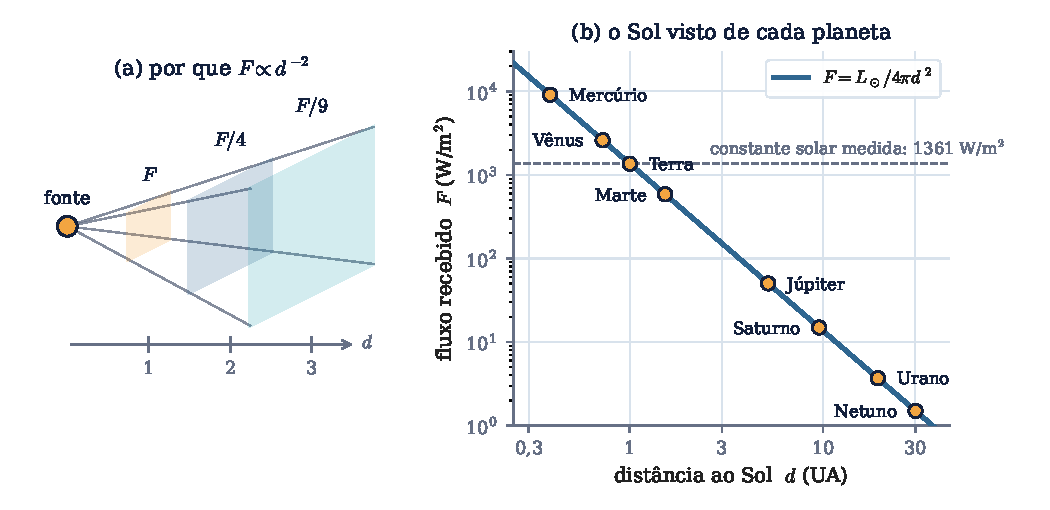
\includegraphics[width=\textwidth]{inverso_quadrado.pdf}
\caption{\textbf{Lei do inverso do quadrado.} \textbf{(a)} A razão é puramente geométrica: a energia que atravessa um quadrado a distância $1$ se espalha por quatro quadrados iguais a distância $2$ e por nove a distância $3$. Nada é absorvido no caminho --- apenas diluído. \textbf{(b)} A mesma lei aplicada ao Sol, com $F=L_\odot/4\pi d^{\,2}$ e $L_\odot=3{,}828\times10^{26}\,\mathrm{W}$, avaliada nas distâncias médias dos planetas. A conta devolve $1361\,\mathrm{W/m^2}$ na órbita da Terra, exatamente a constante solar medida por satélites --- uma verificação, não um ajuste. E explica por que sondas para o Sistema Solar exterior abandonam painéis solares: em Netuno chega $1{,}5\,\mathrm{W/m^2}$, novecentas vezes menos que aqui.}
\end{figure}

A escala de magnitudes preserva a tradição histórica de classificar estrelas por brilho aparente, mas com definição logarítmica moderna. Uma diferença de 5 magnitudes corresponde a um fator 100 em fluxo. Isso significa que pequenas diferenças numéricas em magnitude podem representar grandes diferenças físicas. A magnitude aparente mede o que chega até nós; a magnitude absoluta mede o brilho que o objeto teria a 10 parsecs. A diferença entre as duas está ligada ao módulo de distância, uma relação simples que aparece repetidamente em astrofísica estelar e extragaláctica.

Para interpretar observações, também precisamos lembrar que a luz pode ser modificada no caminho. Poeira interestelar absorve e espalha radiação, afetando mais fortemente comprimentos de onda curtos. O resultado é extinção e avermelhamento: o objeto parece mais fraco e mais vermelho do que seria sem poeira. Um erro comum é atribuir toda cor observada apenas à temperatura. Em muitos contextos, especialmente no plano da Via Láctea e em regiões de formação estelar, é necessário separar cor intrínseca e efeito do meio.

\textbf{Exemplo guiado.} Imagine duas estrelas com mesma luminosidade, mas uma delas está três vezes mais distante. O fluxo observado da estrela distante será nove vezes menor, porque o fluxo cai com o quadrado da distância. Em magnitudes, essa diferença é
\[
\Delta m=-2{,}5\log_{10}(F_2/F_1).
\]
Como $F_2/F_1=1/9$, obtemos $\Delta m\simeq2{,}4$. A estrela mais distante parece cerca de 2,4 magnitudes mais fraca, mesmo sendo fisicamente igual. Este exemplo mostra por que brilho aparente sozinho raramente basta.

\textbf{Perguntas para discussão.}
\begin{itemize}
\item Por que um mapa celeste é bidimensional, enquanto a Galáxia é tridimensional?
\item Que hipóteses entram ao transformar fluxo em luminosidade?
\item Como poeira pode imitar efeitos que parecem ser de temperatura ou distância?
\item Por que escalas logarítmicas aparecem naturalmente em astronomia?
\end{itemize}

\textbf{Para praticar.} Escolha uma estrela brilhante visível no céu da estação. Pesquise sua magnitude aparente, distância aproximada e tipo espectral. Estime sua magnitude absoluta e compare com o Sol. Separe três ideias: aparência no céu, luminosidade intrínseca e posição física no espaço. O resultado costuma ser revelador: algumas estrelas famosas são brilhantes por estarem próximas; outras são brilhantes porque são intrinsicamente enormes ou muito luminosas.

\begin{lessonblock}[borderline west={2pt}{0pt}{astroGold}]{Dedução curta: fluxo, luminosidade e módulo de distância}
Se uma fonte emite luminosidade total $L$ de modo aproximadamente isotrópico, essa energia atravessa uma esfera de raio $d$ e área $4\pi d^2$. O fluxo medido por unidade de área é, portanto,
\[
F=\frac{L}{4\pi d^2}.
\]
A escala de magnitudes é definida por
\[
m_2-m_1=-2{,}5\log_{10}\left(\frac{F_2}{F_1}\right).
\]
Comparando o fluxo observado a uma distância $d$ com o fluxo que o mesmo objeto teria a $10\,\mathrm{pc}$, obtemos o módulo de distância:
\[
m-M=5\log_{10}\left(\frac{d}{10\,\mathrm{pc}}\right).
\]
Essa dedução mostra onde entram as hipóteses: emissão isotrópica, ausência de extinção e distância em parsecs. Quando houver poeira, a forma observacional passa a incluir uma correção $A$: $m-M=5\log_{10}(d/10\,\mathrm{pc})+A$.
\end{lessonblock}

\begin{lessonblock}{Exemplo de aplicação: distância por módulo}
Uma Cefeida em uma galáxia próxima tem magnitude aparente média $m=24{,}0$. Pela relação período-luminosidade, estima-se magnitude absoluta $M=-4{,}0$. Ignorando extinção,
\[
24-(-4)=5\log_{10}(d/10\,\mathrm{pc}),
\]
logo $28=5\log_{10}(d/10\,\mathrm{pc})$ e $\log_{10}(d/10)=5{,}6$. Portanto $d\simeq10^{6{,}6}\,\mathrm{pc}\simeq4{,}0\,\mathrm{Mpc}$. Uma extinção de apenas $0{,}2$ magnitude já deslocaria a distância inferida; por isso calibração fotométrica e poeira não são detalhes cosméticos.
\end{lessonblock}

\subsection*{Laboratório}
\addcontentsline{toc}{subsection}{Laboratório -- Capítulo 1}
O laboratório interativo deste capítulo está disponível em:

\begin{center}
\url{https://rafaelcrdelima.github.io/Astronomia/laboratorio-capitulo-1/}
\end{center}

Neste laboratório você trabalhará como em uma pequena campanha observacional. Cada acesso ao painel gera um catálogo diferente, de modo que os números não serão iguais para todos os grupos. O objetivo é medir posições em datas diferentes, exportar o catálogo, transformar observáveis em grandezas físicas e justificar as inferências feitas.

\begin{lessonblock}[borderline west={2pt}{0pt}{astroGold}]{Roteiro de experimentos}
\textbf{Preparação dos dados.} Abra o laboratório, selecione uma estrela no mapa e varie a data de observação. Use a opção de sobrepor uma data oposta para visualizar o deslocamento anual da estrela em relação ao grid e às estrelas de referência. Depois use o botão \textit{Exportar CSV}. O arquivo contém paralaxe medida, erro de paralaxe, posições simuladas em janeiro e julho, magnitude nos filtros $B$, $V$ e $R$, magnitude absoluta inferida, cor observada, extinção $A_V$ e luminosidade. Use pelo menos 8 estrelas do catálogo para a análise.

\textbf{Experimento 1: paralaxe por duas épocas.}
Para cada uma das 8 estrelas escolhidas, use as colunas de posição em janeiro e julho para calcular o deslocamento angular no mapa:
\[
\Delta_{\rm px}=\sqrt{(x_{\rm jul}-x_{\rm jan})^2+(y_{\rm jul}-y_{\rm jan})^2}.
\]
No laboratório, a escala do mapa é indicada em mas por pixel. Estime a paralaxe por:
\[
p_{\rm grid}(\mathrm{mas})=\frac{\Delta_{\rm px}}{2}\,s_{\rm mapa}.
\]
Compare $p_{\rm grid}$ com a paralaxe exportada no CSV. Em seguida calcule a distância:
\[
d(\mathrm{pc})=\frac{1000}{p(\mathrm{mas})}.
\]
Calcule também a incerteza aproximada:
\[
\sigma_d\simeq d\,\frac{\sigma_p}{p}.
\]
Entregue uma tabela com $\Delta_{\rm px}$, $p_{\rm grid}$, $p$, $\sigma_p$, $d$ e $\sigma_d$. Identifique a estrela com maior erro relativo de distância e explique numericamente por que paralaxes pequenas tornam a distância menos confiável.

\textbf{Experimento 2: magnitude absoluta.}
Usando a magnitude aparente $m$, a distância inferida $d$ e a extinção $A_V$, calcule para as mesmas estrelas:
\[
M=m-5\log_{10}\left(\frac{d}{10\,\mathrm{pc}}\right)-A_V.
\]
Compare seu valor de $M$ com a coluna de magnitude absoluta inferida no arquivo exportado. Registre a diferença absoluta $|\Delta M|$ para cada estrela. Se houver diferença relevante, verifique arredondamento, uso de parsec e inclusão de $A_V$.

\textbf{Experimento 3: luminosidade a partir de magnitude.}
Converta magnitude absoluta em luminosidade relativa ao Sol usando $M_{\odot,V}=4{,}83$:
\[
\frac{L}{L_\odot}=10^{(4{,}83-M)/2{,}5}.
\]
Ordene as 8 estrelas por luminosidade. Depois ordene as mesmas estrelas por magnitude aparente. As duas ordenações coincidem? Escolha dois casos em que não coincidam e explique, com números, se a diferença vem principalmente de distância, luminosidade intrínseca ou extinção.

\textbf{Experimento 4: fotometria em filtros.}
Para as mesmas 8 estrelas, registre $m_B$, $m_V$ e $m_R$. Calcule o índice de cor:
\[
B-V=m_B-m_V.
\]
Compare estrelas com $B-V$ pequeno e grande. Interprete, com números, quais objetos parecem mais azuis ou mais vermelhos. Discuta por que cor observada não mede apenas temperatura: poeira e extinção também entram na interpretação.

\textbf{Experimento 5: brilho aparente versus distância.}
Escolha pares de estrelas com luminosidades inferidas parecidas, mas distâncias diferentes. Para cada par, compare os fluxos relativos com a previsão aproximada da lei do inverso do quadrado:
\[
\frac{F_1}{F_2}\simeq\frac{L_1}{L_2}\left(\frac{d_2}{d_1}\right)^2\,10^{-0{,}4(A_{V,1}-A_{V,2})}.
\]
Calcule pelo menos três razões de fluxo previstas e compare com o CSV. Interprete quando a diferença é dominada por distância, luminosidade intrínseca ou extinção.
\end{lessonblock}

\begin{lessonblock}{Formato da entrega}
A entrega deve conter:
\begin{enumerate}
\item uma tabela com as 8 estrelas analisadas e as grandezas calculadas;
\item pelo menos dois gráficos feitos a partir do CSV: um de deslocamento/paralaxe e outro de magnitude ou luminosidade versus distância;
\item as contas dos cinco experimentos, com unidades;
\item uma interpretação curta separando observáveis, grandezas inferidas e hipóteses usadas;
\item uma conclusão respondendo: por que brilho aparente sozinho não permite saber se uma estrela é fisicamente luminosa?
\end{enumerate}
As respostas devem ser numéricas. Frases como ``a estrela está longe'' ou ``a poeira atrapalha'' só contam se vierem acompanhadas de valores calculados.
\end{lessonblock}

\begin{lessonblock}[borderline west={2pt}{0pt}{astroGold}]{Laboratório de dados 1 -- distâncias e magnitudes com o Gaia}
\textbf{Arquivo:} \texttt{01\_gaia\_estrelas\_25pc.csv} --- 2000 estrelas reais a menos de $25\,\mathrm{pc}$ do Sol, medidas pela missão Gaia. Colunas: \texttt{paralaxe\_mas}, \texttt{erro\_paralaxe\_mas}, \texttt{G\_mag}, \texttt{BP\_RP}.

\textbf{Física.} A paralaxe dá a distância por geometria pura, e a distância converte brilho aparente em brilho intrínseco:
\[
d\,[\mathrm{pc}]=\frac{1000}{p\,[\mathrm{mas}]},\qquad
M=m-5\log_{10}\!\left(\frac{d}{\mathrm{pc}}\right)+5.
\]

\textbf{Roteiro.}
\begin{enumerate}
\item Crie uma coluna de distância. No Excel: \texttt{=1000/B2}. Em Python: \texttt{df["d"]=1000/df.paralaxe\_mas}.
\item Crie a coluna de magnitude absoluta: \texttt{=D2-5*LOG10(F2)+5}.
\item Faça o gráfico de dispersão de $M$ (eixo $y$, invertido) contra \texttt{BP\_RP} (eixo $x$). Você acaba de construir um diagrama HR com dados próprios.
\item Identifique a sequência principal e o grupo isolado embaixo à esquerda. Quantas estrelas há em cada grupo?
\item Propague a incerteza: $\sigma_d/d=\sigma_p/p$. Para quantas estrelas a distância é melhor que $1\%$?
\end{enumerate}

\textbf{Entrega.} O diagrama, a contagem dos dois grupos e uma resposta curta: por que uma amostra limitada por volume, como esta, contém tantas estrelas fracas e quase nenhuma gigante?

\textbf{Confira.} A estrela mais próxima da lista tem $p\simeq768\,\mathrm{mas}$, ou seja $d\simeq1{,}30\,\mathrm{pc}$ --- é Proxima Centauri.
\end{lessonblock}

\newpage
\section*{Capítulo 2 -- Mecânica celeste e gravitação}
\addcontentsline{toc}{section}{Capítulo 2 -- Mecânica celeste e gravitação}
\aberturabloco{Fundamentos quantitativos}{Este capítulo reforça a passagem da geometria observacional para a dinâmica gravitacional. A pergunta central é simples: como movimentos observados revelam massa?}{Trabalhe sempre com desenho, unidades e ordem de grandeza antes de substituir números. Em gravitação, uma conta dimensional bem feita costuma revelar metade da física.}

Órbitas são uma das ferramentas mais poderosas da astrofísica porque a gravidade transforma movimento em medida de massa. No caso circular simples, igualamos força gravitacional e aceleração centrípeta:
\[
\frac{GMm}{r^2}=\frac{mv^2}{r}.
\]
Daí vem $v^2=GM/r$ e $M=rv^2/G$. Essa relação aparece em muitos lugares: planetas ao redor do Sol, estrelas ao redor do centro galáctico, gás em discos de galáxias e matéria em aglomerados. A forma exata muda com geometria e distribuição de massa, mas a ideia permanece: movimento orbital é uma balança gravitacional.

A terceira lei de Kepler generalizada,
\[
P^2=\frac{4\pi^2a^3}{G(M_1+M_2)},
\]
mostra que período e tamanho orbital medem a soma das massas. Em sistemas planetários, normalmente $M_\star\gg M_p$, e a massa do planeta pouco altera o período. Em binárias estelares, as duas massas podem ser comparáveis, e o problema fica mais rico. Por isso estrelas binárias são tão importantes no Carroll \& Ostlie: elas fornecem massas reais, não apenas estimativas teóricas.

\observaveis{período orbital, semieixo maior angular, velocidade radial}{massa total, inclinação orbital, separação física}{distância calibrada, órbita aproximadamente kepleriana, identificação correta dos componentes}{Que parte da massa foi medida dinamicamente e que parte depende de uma hipótese geométrica?}

\begin{figure}[htbp]
\centering
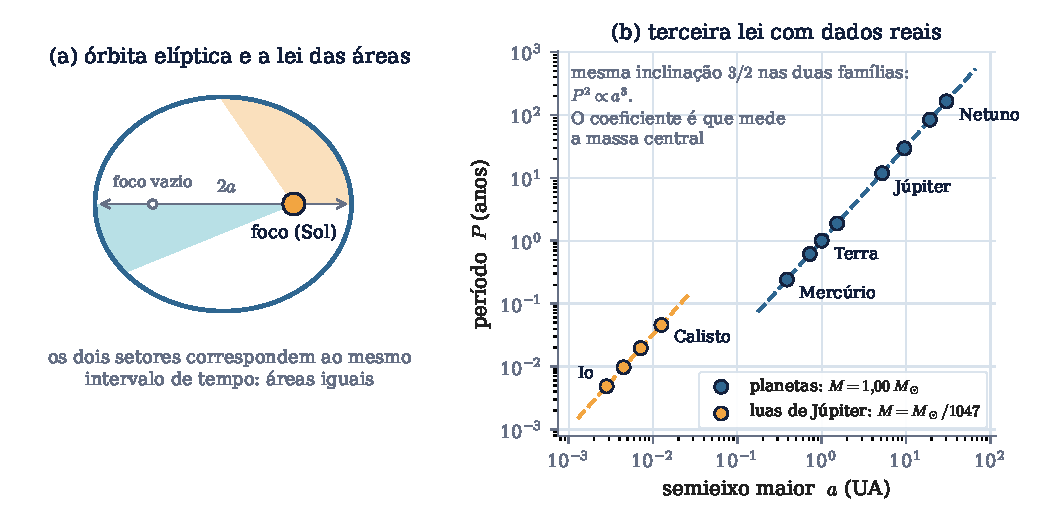
\includegraphics[width=\textwidth]{kepler.pdf}
\caption{\textbf{As leis de Kepler.} \textbf{(a)} Órbita de excentricidade $0{,}55$ obtida resolvendo a equação de Kepler $M=E-e\,\mathrm{sen}\,E$. O corpo central ocupa um foco, o outro fica vazio, e os dois setores sombreados --- percorridos no mesmo intervalo de tempo --- têm a mesma área: perto do periélio o planeta corre mais e cobre um ângulo grande com raio curto; perto do afélio faz o oposto. \textbf{(b)} A terceira lei com dados tabelados: os oito planetas em torno do Sol e os quatro satélites galileanos em torno de Júpiter. As duas famílias caem sobre retas de mesma inclinação $3/2$ mas coeficientes diferentes, e é o coeficiente que carrega a física: aplicando $M=4\pi^2a^3/GP^2$ aos planetas obtém-se $1{,}00\,M_\odot$; aplicando às luas, $1{,}90\times10^{27}\,\mathrm{kg}$, a massa de Júpiter, cerca de $M_\odot/1047$. A mesma lei, medindo dois corpos centrais diferentes.}
\end{figure}

\textbf{Exemplo resolvido.} Um planeta orbita uma estrela em $P=1$ ano com $a=1\,\mathrm{UA}$. Como esse é o caso da Terra, a massa inferida é $1M_\odot$. Se outro planeta orbita a mesma estrela em $a=4\,\mathrm{UA}$, então $P^2\propto a^3=64$, logo $P=8$ anos. A conta não exigiu conhecer $G$ porque usamos uma calibração solar. Essa é uma lição prática: relações proporcionais são atalhos poderosos quando a referência é bem escolhida.

\textbf{Erros comuns.} Não confunda raio orbital instantâneo com semieixo maior; não use a forma circular quando a excentricidade é essencial; não esqueça a inclinação em velocidades radiais; não trate velocidade projetada como velocidade total sem justificativa.

\begin{lessonblock}[borderline west={2pt}{0pt}{astroGold}]{Dedução curta: terceira lei de Kepler}
Para uma órbita circular, $v=2\pi r/P$. Igualando gravidade e aceleração centrípeta,
\[
\frac{G(M_1+M_2)}{r^2}=\frac{v^2}{r}=\frac{4\pi^2r}{P^2}.
\]
Reorganizando,
\[
P^2=\frac{4\pi^2r^3}{G(M_1+M_2)}.
\]
Para órbitas elípticas, o raio circular $r$ é substituído pelo semieixo maior $a$. A forma final é a mesma já apresentada:
\[
P^2=\frac{4\pi^2a^3}{G(M_1+M_2)}.
\]
O detalhe conceitual importante é que a lei mede a massa total do sistema, não apenas a massa do corpo central, embora em planetas comuns a massa da estrela domine.
\end{lessonblock}

\begin{lessonblock}{Exemplo de aplicação: velocidade de escape}
A velocidade de escape vem de igualar energia cinética inicial e energia gravitacional necessária para escapar:
\[
\frac{1}{2}mv_{\rm esc}^2=\frac{GMm}{R}
\quad\Rightarrow\quad
v_{\rm esc}=\sqrt{\frac{2GM}{R}}.
\]
Para a Terra, $v_{\rm esc}\simeq11{,}2\,\mathrm{km\,s^{-1}}$. Para uma anã branca com massa solar e raio terrestre, a mesma fórmula daria milhares de quilômetros por segundo. A equação é newtoniana, mas já aponta para o regime em que relatividade e compactação se tornam inevitáveis.
\end{lessonblock}

\begin{lessonblock}{Do céu observado à órbita}
O laboratório deste capítulo não mostra a órbita vista de cima. Ele mostra o que um observador mede no céu: direções. Por isso é essencial separar três tipos de grandezas:
\begin{itemize}
\item \textbf{coordenadas eclípticas} $(\lambda,\beta)$: longitude e latitude medidas em relação ao plano da órbita da Terra;
\item \textbf{coordenadas equatoriais} $(\alpha,\delta)$: ascensão reta e declinação, úteis para localizar objetos em catálogos e telescópios;
\item \textbf{coordenadas horizontais} $(A,h)$: azimute e altura, que dependem do local, da hora sideral e da latitude do observador.
\end{itemize}
O mesmo planeta tem praticamente a mesma longitude eclíptica geocêntrica em uma data dada, mas sua altura no horizonte muda quando mudamos a hora ou a latitude. Assim, $\lambda(t)$ é boa para estudar a dinâmica orbital, enquanto $h(t)$ e $A(t)$ respondem à pergunta observacional: \textit{dá para ver esse objeto agora?}

No céu local, a altura $h$ de um objeto com ascensão reta $\alpha$ e declinação $\delta$ é dada por
\[
\sin h=\sin\phi\,\sin\delta+\cos\phi\,\cos\delta\,\cos H,
\]
onde $\phi$ é a latitude do observador e $H$ é o ângulo horário:
\[
H=\theta_{\rm LST}-\alpha.
\]
Aqui $\theta_{\rm LST}$ é a hora sideral local. Um objeto está acima do horizonte quando $h>0^\circ$. Essa equação explica por que um planeta pode estar em posição orbital interessante e, ainda assim, não ser observável para um dado observador.
\end{lessonblock}

\textbf{Exemplo: janela de observação.} Suponha um planeta com $\delta=10^\circ$, observado de Joinville, aproximadamente $\phi=-26^\circ$. Se no instante considerado $H=0^\circ$, então
\[
\sin h=\sin(-26^\circ)\sin(10^\circ)+\cos(-26^\circ)\cos(10^\circ)\cos(0^\circ).
\]
Numericamente, $\sin h\simeq -0{,}076+0{,}885=0{,}809$, logo $h\simeq54^\circ$. O planeta está alto no céu. Se seis horas siderais depois $H=90^\circ$, o termo com cosseno desaparece:
\[
\sin h\simeq \sin(-26^\circ)\sin(10^\circ)\simeq -0{,}076,
\]
então $h\simeq -4{,}4^\circ$: o mesmo planeta estaria abaixo do horizonte. O laboratório permite verificar esse efeito variando a hora sideral.

\begin{lessonblock}[borderline west={2pt}{0pt}{astroBlue}]{Elongação, oposição e conjunção}
A \textbf{elongação solar} $E$ é a separação angular aparente entre o planeta e o Sol no céu. Em termos de longitudes eclípticas geocêntricas, uma aproximação útil quando as latitudes eclípticas são pequenas é
\[
E\simeq |\lambda_p-\lambda_\odot|,
\]
tomando o menor ângulo entre $0^\circ$ e $180^\circ$. Na prática, use
\[
E=\left|\operatorname{wrap}_{180}(\lambda_p-\lambda_\odot)\right|,
\]
onde $\operatorname{wrap}_{180}$ recoloca a diferença angular no intervalo $[-180^\circ,180^\circ]$.

Para planetas externos, uma \textbf{oposição} ocorre quando $E\simeq180^\circ$: Sol e planeta aparecem em lados opostos do céu. A oposição é especialmente importante porque o planeta tende a estar mais brilhante e observável por boa parte da noite. Uma \textbf{conjunção} ocorre quando $E\simeq0^\circ$: planeta e Sol aparecem quase na mesma direção, o que dificulta ou impossibilita a observação visual.

Para planetas internos, como Mercúrio e Vênus, a elongação nunca chega a $180^\circ$. Eles ficam sempre angularmente próximos do Sol. A maior elongação é uma pista geométrica do tamanho de sua órbita.
\end{lessonblock}

\textbf{Exemplo: identificando oposição em uma tabela.} Imagine que, para Marte, o laboratório exportou:
\[
\begin{array}{c|c}
\text{dia} & E\\
\hline
720 & 171^\circ\\
735 & 178^\circ\\
750 & 176^\circ
\end{array}
\]
A melhor estimativa discreta da oposição é dia $735$. Se a oposição seguinte ocorre no dia $1515$, então o período sinódico estimado é
\[
S=1515-735=780\ \text{dias}=2{,}14\ \text{anos}.
\]
Esse número não é o período orbital de Marte em torno do Sol; é o tempo entre configurações Terra--Sol--Marte parecidas vistas da Terra.

\begin{lessonblock}{Período sinódico e período sideral}
O período sideral $P$ é o período orbital real em relação às estrelas distantes. O período sinódico $S$ é o tempo para que a configuração aparente observada da Terra se repita, por exemplo de uma oposição à próxima. Para movimentos médios circulares, a velocidade angular média é
\[
n=\frac{2\pi}{P}.
\]
Para um planeta externo, a Terra, mais interna, ``alcança'' o planeta. A taxa relativa é
\[
n_\oplus-n_p=\frac{2\pi}{S}.
\]
Como $P_\oplus=1$ ano,
\[
\frac{1}{S}=1-\frac{1}{P_p}.
\]
Reorganizando,
\[
\frac{1}{P_p}=1-\frac{1}{S}
\quad\Rightarrow\quad
P_p=\frac{1}{1-1/S},
\]
com $P_p$ e $S$ em anos. Para planetas internos, a ordem se inverte:
\[
\frac{1}{S}=\frac{1}{P_p}-1
\quad\Rightarrow\quad
\frac{1}{P_p}=1+\frac{1}{S}.
\]
No laboratório, use a forma de planeta externo para Marte, Júpiter e Saturno.
\end{lessonblock}

\textbf{Exemplo: período de Marte a partir de oposições.} Usando $S=2{,}14$ anos,
\[
\frac{1}{P}=1-\frac{1}{2{,}14}=1-0{,}467=0{,}533.
\]
Portanto,
\[
P\simeq1{,}88\ \text{anos}.
\]
Esse valor é próximo do período sideral real de Marte. O ponto didático é importante: medindo apenas datas de oposição, que são observáveis angulares, chegamos a uma propriedade orbital heliocêntrica.

\begin{lessonblock}{Lei de Kepler em unidades astronômicas}
Para planetas orbitando o Sol, é muito conveniente usar anos, unidades astronômicas e massas solares. Nestas unidades,
\[
P^2=a^3
\]
para objetos de massa desprezível comparada ao Sol. Assim,
\[
a=P^{2/3}.
\]
Essa forma é a que aparece no roteiro do laboratório. Ela é uma versão adimensional da terceira lei:
\[
P^2=\frac{4\pi^2a^3}{GM_\odot}.
\]
Quando usamos $P=1\,\mathrm{ano}$ e $a=1\,\mathrm{UA}$ para a Terra, o fator $4\pi^2/(GM_\odot)$ fica automaticamente embutido na escolha de unidades.
\end{lessonblock}

\textbf{Exemplo: semieixo maior de Marte.} Com $P=1{,}88$ anos,
\[
a=P^{2/3}=1{,}88^{2/3}.
\]
Uma forma prática é calcular primeiro $P^2$:
\[
P^2\simeq3{,}53.
\]
Como $a^3=P^2$, queremos a raiz cúbica de $3{,}53$:
\[
a\simeq1{,}52\ \mathrm{UA}.
\]
O laboratório deve levar a um valor próximo disso se as oposições forem bem escolhidas.

\begin{lessonblock}{Movimento direto e retrógrado}
Quando acompanhamos a longitude eclíptica $\lambda(t)$ de um planeta externo, normalmente ela aumenta com o tempo em relação ao fundo de estrelas. Esse é o movimento direto. Perto da oposição, porém, a Terra passa o planeta por dentro da órbita. A direção aparente pode inverter por algumas semanas ou meses: é o movimento retrógrado.

Em uma tabela discreta, calcule diferenças sucessivas:
\[
\Delta\lambda_i=\lambda_{i+1}-\lambda_i.
\]
Como longitude é angular, trate a passagem por $0^\circ$ com cuidado usando novamente uma diferença embrulhada:
\[
\Delta\lambda_i=\operatorname{wrap}_{180}(\lambda_{i+1}-\lambda_i).
\]
Se $\Delta\lambda_i>0$, o movimento naquele intervalo é direto; se $\Delta\lambda_i<0$, é retrógrado. O gráfico $\lambda(t)$ deve mostrar uma mudança de inclinação nos intervalos retrógrados.
\end{lessonblock}

\textbf{Exemplo: detectando retrogradação.} Considere observações de Marte:
\[
\begin{array}{c|c|c}
\text{dia} & \lambda & \Delta\lambda\\
\hline
0 & 142^\circ & \\
30 & 150^\circ & +8^\circ\\
60 & 154^\circ & +4^\circ\\
90 & 151^\circ & -3^\circ\\
120 & 146^\circ & -5^\circ\\
150 & 148^\circ & +2^\circ
\end{array}
\]
O intervalo entre os dias 60 e 120 é retrógrado. Em uma entrega, não basta dizer ``Marte voltou'': indique os intervalos e os valores de $\Delta\lambda$ que sustentam a conclusão.

\begin{lessonblock}[borderline west={2pt}{0pt}{astroGold}]{Maior elongação de planetas internos}
Para um planeta interno em órbita circular, a maior elongação ocorre quando a linha de visada Terra--planeta é tangente à órbita do planeta. No triângulo Sol--Terra--planeta, o ângulo no planeta é $90^\circ$. Se a distância Terra--Sol é $1\,\mathrm{UA}$ e o raio orbital do planeta é $a$, então
\[
\sin E_{\max}\simeq \frac{a}{1\,\mathrm{UA}}.
\]
Logo,
\[
a\simeq \sin E_{\max}\ \mathrm{UA}.
\]
Essa dedução é aproximada: órbitas reais são elípticas e inclinadas, mas a relação captura a geometria básica.
\end{lessonblock}

\textbf{Exemplo: órbita de Vênus por maior elongação.} Se o laboratório mostra $E_{\max}\simeq46^\circ$, então
\[
a\simeq\sin 46^\circ\simeq0{,}72\ \mathrm{UA}.
\]
Para Mercúrio, uma maior elongação típica de $23^\circ$ dá
\[
a\simeq\sin 23^\circ\simeq0{,}39\ \mathrm{UA}.
\]
Assim, mesmo sem ver a órbita de cima, a geometria angular já indica que Vênus orbita mais longe do Sol do que Mercúrio.

\begin{lessonblock}{Como apresentar contas com dados do laboratório}
Para cada grandeza estimada, deixe claro:
\begin{enumerate}
\item quais colunas do CSV foram usadas;
\item quais observações foram selecionadas;
\item qual equação foi aplicada;
\item em que unidade está o resultado;
\item qual é a interpretação física.
\end{enumerate}
Um bom padrão de tabela para o teste de Kepler é:
\[
\begin{array}{c|c|c|c|c}
\text{planeta} & S\ (\text{anos}) & P\ (\text{anos}) & a=P^{2/3}\ (\mathrm{UA}) & P^2/a^3\\
\hline
\text{Marte} & 2{,}14 & 1{,}88 & 1{,}52 & 1{,}00
\end{array}
\]
Se os dados forem aproximados, $P^2/a^3$ não precisa dar exatamente $1$, mas deve ficar próximo. Diferenças grandes indicam erro de unidade, oposição mal identificada ou confusão entre período sinódico e sideral.
\end{lessonblock}

\subsection*{Laboratório}
\addcontentsline{toc}{subsection}{Laboratório -- Capítulo 2}
O laboratório interativo deste capítulo está disponível em:

\begin{center}
\url{https://rafaelcrdelima.github.io/Astronomia/laboratorio-capitulo-2/}
\end{center}

Neste laboratório você trabalhará como um observador pré-telescópico ou do início da astronomia moderna. O painel não entrega a órbita vista de cima: ele mostra posições aparentes de planetas no céu, como longitude e latitude eclípticas, ascensão reta, declinação, altura e elongação solar. A tarefa é construir, a partir dessas medidas angulares, a evidência que levou às leis de Kepler.

\begin{lessonblock}[borderline west={2pt}{0pt}{astroGold}]{Roteiro de experimentos}
\textbf{Preparação dos dados.} Abra o laboratório, escolha um planeta, varie a data da observação e use \textit{Registrar observação}. Repita o procedimento por muitas datas. O CSV exportado contém data, planeta, longitude e latitude eclípticas, ascensão reta, declinação, azimute, altura e elongação solar. Use a régua angular do mapa para medir separações no céu sempre que precisar comparar duas posições.

\textbf{Experimento 1: caderno de observações de Marte.}
Registre a longitude eclíptica de Marte a cada 20 ou 30 dias durante pelo menos três anos simulados. Faça um gráfico $\lambda(t)$. Identifique intervalos de movimento direto e movimento retrógrado. Explique por que uma descrição geocêntrica simples exigiria um movimento aparente complicado.

\textbf{Experimento 2: período sinódico e período sideral.}
Para Marte, Júpiter ou Saturno, encontre duas oposições sucessivas, isto é, datas em que a elongação solar fica próxima de $180^\circ$. A diferença entre essas datas é o período sinódico $S$. Para um planeta externo, calcule o período sideral:
\[
\frac{1}{P}=1-\frac{1}{S},
\]
com $P$ e $S$ em anos. Compare seu $P$ com o valor inferido visualmente pela repetição do padrão no gráfico $\lambda(t)$.

\textbf{Experimento 3: terceira lei de Kepler.}
Use o período sideral obtido para planetas externos e estime o semieixo maior relativo:
\[
a=P^{2/3},
\]
em unidades de UA quando $P$ está em anos. Monte uma tabela com $P$, $P^2$, $a$ e $a^3$ para pelo menos Marte, Júpiter e Saturno. Verifique numericamente se $P^2/a^3$ é aproximadamente constante.

\textbf{Experimento 4: planetas internos e maior elongação.}
Para Mercúrio ou Vênus, registre a elongação solar em muitas datas. Encontre a maior elongação $E_{\max}$. Para uma órbita aproximadamente circular interna, estime:
\[
a\simeq\sin(E_{\max}).
\]
Compare Mercúrio e Vênus. Qual deles fica mais distante angularmente do Sol no céu? O que isso indica sobre seu raio orbital?

\textbf{Experimento 5: altura, ascensão reta e janela observacional.}
Escolha um planeta e varie a hora sideral local e a latitude do observador. Registre ascensão reta, declinação e altura. Determine em que horários o planeta está acima do horizonte. Interprete por que uma posição orbital favorável não garante observação se o objeto estiver baixo ou abaixo do horizonte.
\end{lessonblock}

\begin{lessonblock}{Formato da entrega}
A entrega deve conter o caderno de dados exportado, um gráfico $\lambda(t)$ para Marte, uma estimativa de período sinódico e sideral para pelo menos um planeta externo, uma tabela testando $P^2/a^3$, uma estimativa de $a$ por maior elongação para Mercúrio ou Vênus, e uma interpretação curta respondendo: como medidas puramente angulares podem revelar a arquitetura orbital do Sistema Solar?
\end{lessonblock}

\begin{lessonblock}{Extensão quantitativa: massa solar}
Depois de obter $a$ e $P$, a terceira lei na forma dimensional permite inferir a massa central:
\[
M_\odot=\frac{4\pi^2a^3}{GP^2}.
\]
Use $a=1\,\mathrm{UA}$ e $P=1\,\mathrm{ano}$ para recuperar a escala de massa do Sol. Essa etapa mostra a ponte entre astronomia de posição e dinâmica gravitacional.
\end{lessonblock}
\begin{lessonblock}[borderline west={2pt}{0pt}{astroGold}]{Laboratório de dados 2 -- pesar o Sol, Júpiter e Saturno}
\textbf{Arquivo:} \texttt{02\_terceira\_lei\_kepler.csv} --- semieixo maior e período de 21 corpos reais, orbitando quatro centros diferentes.

\textbf{Física.} A terceira lei de Kepler na forma newtoniana é uma balança gravitacional:
\[
M=\frac{4\pi^{2}a^{3}}{GP^{2}}.
\]
Em unidades astronômicas e anos, com massa em massas solares, ela vira simplesmente $M=a^{3}/P^{2}$.

\textbf{Roteiro.}
\begin{enumerate}
\item Calcule $a^{3}/P^{2}$ para cada corpo. No Excel: \texttt{=C2\^{}3/D2\^{}2}.
\item Agrupe por coluna \texttt{orbita\_em\_torno\_de} e tire a média de cada grupo. Você obteve a massa de cada corpo central, em massas solares.
\item Converta as massas de Júpiter e Saturno para quilogramas e compare com valores tabelados.
\item Faça o gráfico de $\log P$ contra $\log a$ com todos os corpos, colorindo por sistema. Confirme que a inclinação é $3/2$ e explique por que as retas são paralelas mas deslocadas.
\end{enumerate}

\textbf{Entrega.} A tabela com as quatro massas centrais obtidas, o gráfico log-log e uma frase sobre o que o deslocamento vertical entre as retas significa fisicamente.

\textbf{Confira.} Pelos planetas você deve obter $\simeq1{,}00\,M_\odot$; pelas luas galileanas, $\simeq9{,}5\times10^{-4}\,M_\odot$, isto é, $M_\odot/1047$ --- a massa de Júpiter.
\end{lessonblock}

\newpage
\section*{Capítulo 3 -- Radiação, corpo negro e espectros}
\addcontentsline{toc}{section}{Capítulo 3 -- Radiação, corpo negro e espectros}
A luz é o mensageiro mais importante da astrofísica. Ela transporta energia, momento, direção, polarização e informação espectral. Um único fóton possui energia $E=h\nu=hc/\lambda$, de modo que comprimentos de onda menores correspondem a fótons mais energéticos. Essa relação conecta cor, temperatura, transições atômicas e processos de alta energia. Quando um telescópio registra luz, ele não está apenas formando uma imagem: está coletando evidências sobre a matéria que emitiu, absorveu ou espalhou essa radiação.

O espectro contínuo de muitos objetos pode ser comparado, em primeira aproximação, à radiação de corpo negro. Um corpo negro ideal absorve e emite radiação de maneira determinada apenas por sua temperatura. A lei de Wien indica que o comprimento de onda de máxima emissão diminui quando a temperatura aumenta:
\[
\lambda_{\max}T\simeq2{,}9\times10^{-3}\,\mathrm{m\,K}.
\]
Por isso estrelas frias têm aparência avermelhada e estrelas quentes emitem mais fortemente em azul e ultravioleta. Essa regra, porém, não deve ser usada mecanicamente: atmosferas reais têm linhas, bandas moleculares, opacidades dependentes do comprimento de onda e efeitos de poeira no caminho.

\begin{figure}[htbp]
\centering
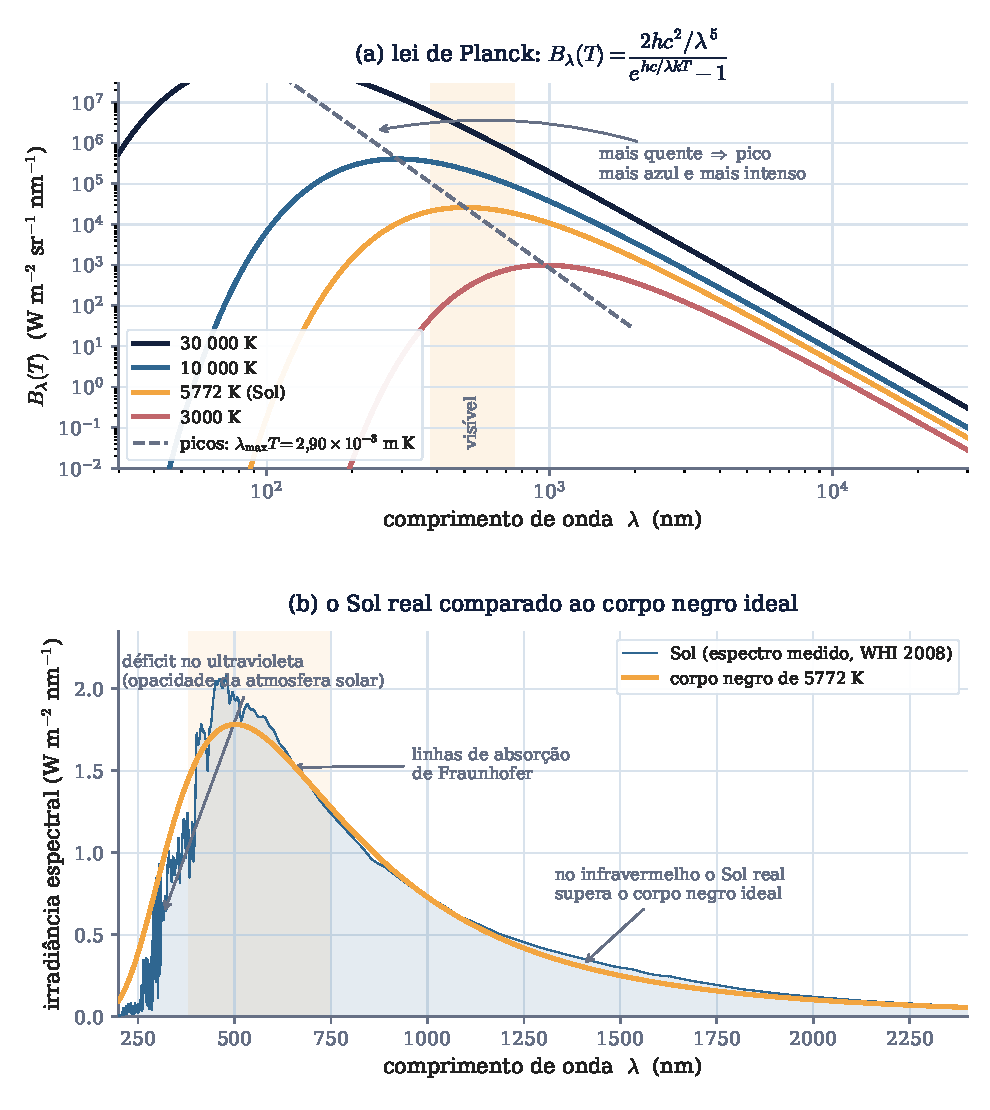
\includegraphics[width=\textwidth]{corpo_negro.pdf}
\caption{\textbf{Corpo negro: o ideal e o real.} \textbf{(a)} Curvas calculadas diretamente da lei de Planck para quatro temperaturas. Em escala log-log o efeito é duplo: o pico se desloca para comprimentos de onda menores (lei de Wien, tracejado ligando os máximos) e toda a curva sobe, porque o fluxo integrado cresce com $T^4$ (lei de Stefan-Boltzmann). Note que nenhuma curva cruza outra: uma estrela mais quente emite mais em \emph{todo} comprimento de onda, e não apenas no azul. \textbf{(b)} O espectro solar realmente medido acima da atmosfera terrestre, comparado ao corpo negro de $5772\,\mathrm{K}$ com o mesmo raio e distância. O envelope é bem reproduzido, mas os desvios são grandes e informativos: entre $200$ e $400\,\mathrm{nm}$ o Sol emite apenas $65\%$ do previsto, porque a opacidade cresce no ultravioleta e a radiação escapa de camadas mais altas e frias; no visível o espectro é recortado pelas linhas de absorção de Fraunhofer; entre $1400$ e $2400\,\mathrm{nm}$ a emissão real supera a ideal em cerca de $19\%$. Corpo negro é um ponto de partida, não uma descrição completa. Dados do painel (b): \textit{Whole Heliosphere Interval reference spectrum} (SORCE/TIMED), LASP/LISIRD, Universidade do Colorado.}
\end{figure}

As linhas espectrais são assinaturas de quantização. Átomos e moléculas só absorvem ou emitem fótons associados a diferenças específicas de energia entre níveis. Uma linha de hidrogênio, cálcio, sódio ou ferro é como uma pista de presença química, mas sua intensidade depende de temperatura, ionização, densidade e opacidade. A ausência de uma linha forte não significa necessariamente ausência do elemento; pode significar que o elemento está em estado de ionização inadequado ou que as condições físicas não favorecem aquela transição.

O efeito Doppler transforma espectros em medidores de movimento. Se uma fonte se aproxima, suas linhas deslocam-se para comprimentos de onda menores; se se afasta, deslocam-se para comprimentos maiores. Para velocidades pequenas comparadas à velocidade da luz, a aproximação
\[
\frac{\Delta\lambda}{\lambda}\simeq\frac{v_r}{c}
\]
permite medir a velocidade radial. Esse método revela binárias espectroscópicas, rotação estelar, expansão de nebulosas, discos de acreção, planetas por velocidade radial e redshifts de galáxias. Em cosmologia, o redshift ganha interpretação ligada à expansão do próprio espaço, mas a ideia observacional continua sendo o deslocamento de linhas.

\begin{lessonblock}{O que o detector realmente mede}
Um espectro observado não começa como ``fluxo físico''. Ele começa como contagens no detector. Para uma exposição de duração $t$, em um comprimento de onda $\lambda$, uma forma simplificada do sinal é
\[
C_{\rm bruto}(\lambda)=t\,R_{\rm inst}(\lambda)\,F_\lambda(\lambda)+D(\lambda)+N(\lambda),
\]
onde $R_{\rm inst}$ é a resposta instrumental, $D$ é dark current e $N$ representa ruído. A redução de dados tenta recuperar algo proporcional ao fluxo:
\[
F_\lambda(\lambda)\propto
\frac{C_{\rm bruto}(\lambda)-D(\lambda)}{t\,R_{\rm inst}(\lambda)}.
\]
No laboratório, os modos ``bruto'', ``subtrair dark'' e ``dark + resposta instrumental'' mostram por que calibração não é detalhe burocrático: ela altera a forma do contínuo e, portanto, a temperatura inferida.
\end{lessonblock}

\begin{lessonblock}[borderline west={2pt}{0pt}{astroGold}]{Corpo negro e temperatura efetiva}
A lei de Planck para radiância espectral pode ser escrita como
\[
B_\lambda(T)=\frac{2hc^2}{\lambda^5}
\frac{1}{e^{hc/(\lambda kT)}-1}.
\]
Em muitos usos didáticos não precisamos ajustar toda a constante de normalização. A forma do contínuo já informa temperatura. A lei de Wien,
\[
\lambda_{\max}T=b,\qquad b=2{,}898\times10^{-3}\,\mathrm{m\,K},
\]
leva a
\[
T\simeq\frac{2{,}898\times10^6}{\lambda_{\max}(\mathrm{nm})}\ \mathrm{K}.
\]
A luminosidade emitida por unidade de área de um corpo negro é dada por Stefan--Boltzmann:
\[
F=\sigma T^4.
\]
Para uma estrela de raio $R$ observada a distância $d$, o fluxo bolométrico observado escala como
\[
f_{\rm bol}=\sigma T^4\left(\frac{R}{d}\right)^2.
\]
Assim, temperatura vem da forma do espectro, enquanto raio e distância entram na normalização do fluxo.
\end{lessonblock}

\textbf{Exemplo: temperatura por Wien.} Se o contínuo calibrado tem pico em $\lambda_{\max}=520\,\mathrm{nm}$, então
\[
T\simeq\frac{2{,}898\times10^6}{520}\simeq5570\,\mathrm{K}.
\]
Se o mesmo espectro bruto, antes da correção instrumental, parecia ter pico em $610\,\mathrm{nm}$, daria
\[
T\simeq4750\,\mathrm{K}.
\]
A diferença não significa que a estrela mudou: significa que a resposta instrumental deformou o contínuo observado.

\begin{lessonblock}{Fotometria em filtros e índice de cor}
Um filtro não mede o fluxo em um único comprimento de onda; ele mede uma média ponderada por uma curva de transmissão $S_X(\lambda)$:
\[
F_X=\frac{\int F_\lambda(\lambda)S_X(\lambda)\,d\lambda}
{\int S_X(\lambda)\,d\lambda}.
\]
Em fotometria astronômica, magnitudes são logarítmicas. Ignorando constantes de ponto zero, a diferença de cor entre duas bandas pode ser estimada por
\[
B-V\simeq -2{,}5\log_{10}\left(\frac{F_B}{F_V}\right).
\]
Valores menores de $B-V$ indicam objeto relativamente mais azul; valores maiores indicam objeto relativamente mais vermelho. Essa interpretação deve ser feita com cuidado, pois poeira interestelar também avermelha a luz.
\end{lessonblock}

\textbf{Exemplo: cor a partir de fluxos.} Se uma observação calibrada fornece $F_B=0{,}42$ e $F_V=0{,}60$ em unidades relativas,
\[
B-V=-2{,}5\log_{10}(0{,}42/0{,}60)
=-2{,}5\log_{10}(0{,}70)\simeq0{,}39.
\]
Se outra estrela tem $F_B/F_V=1{,}20$, então $B-V\simeq-0{,}20$, indicando espectro mais azul e, em geral, temperatura efetiva maior.

\begin{lessonblock}{Linhas espectrais e velocidade radial}
Uma linha espectral tem um comprimento de onda de repouso $\lambda_0$. Se a linha é observada em $\lambda_{\rm obs}$, então
\[
\Delta\lambda=\lambda_{\rm obs}-\lambda_0.
\]
Para velocidades pequenas comparadas a $c$,
\[
v_r\simeq c\,\frac{\Delta\lambda}{\lambda_0}.
\]
Se $v_r>0$, a fonte está se afastando; se $v_r<0$, está se aproximando. Para a linha H$\alpha$,
\[
\lambda_0=656{,}28\,\mathrm{nm}.
\]
Um deslocamento de apenas $0{,}22\,\mathrm{nm}$ já corresponde a
\[
v_r\simeq 3{,}0\times10^5\,\frac{0{,}22}{656{,}28}
\simeq100\,\mathrm{km\,s^{-1}}.
\]
Essa sensibilidade é uma das razões pelas quais espectroscopia é tão poderosa.
\end{lessonblock}

\textbf{Exemplo: H$\alpha$ deslocada.} Se o laboratório mostra o mínimo de H$\alpha$ em $656{,}05\,\mathrm{nm}$,
\[
\Delta\lambda=-0{,}23\,\mathrm{nm}.
\]
Logo,
\[
v_r\simeq 299792\,\frac{-0{,}23}{656{,}28}
\simeq -105\,\mathrm{km\,s^{-1}}.
\]
O sinal negativo indica aproximação. Em uma entrega, sempre informe a linha usada, o comprimento de onda de repouso, o comprimento observado e o sinal da velocidade.

\begin{lessonblock}{Fluxo integrado e comparação entre objetos}
O fluxo bolométrico é a integral do fluxo espectral:
\[
f_{\rm bol}=\int_0^\infty F_\lambda\,d\lambda.
\]
Na prática, com dados discretos em uma faixa limitada, usamos uma soma aproximada:
\[
f_{\rm faixa}\simeq \sum_i F_{\lambda,i}\,\Delta\lambda_i.
\]
Esse valor não é o fluxo bolométrico completo, pois falta radiação fora da faixa observada, mas é útil para comparar objetos observados com o mesmo instrumento e a mesma redução. Estrelas quentes podem emitir muita radiação no ultravioleta, fora da faixa visível; estrelas frias podem emitir parte importante no infravermelho. Portanto, a integral visível deve ser interpretada como fluxo na faixa observada, não como luminosidade total sem correção.
\end{lessonblock}

\begin{lessonblock}{Da imagem ao espectro: abertura e fundo}
Antes de obter um espectro útil, o observador precisa decidir de onde vem a luz do objeto e de onde vem o fundo. Em uma imagem real, a estrela não aparece como um ponto matemático: ela é espalhada pela óptica e pelo detector em uma \textit{função de espalhamento pontual} (PSF). Por isso usamos uma abertura circular em torno da estrela. Se a abertura for pequena demais, perdemos parte da luz; se for grande demais, somamos ruído e luz de fundo desnecessários.

O sinal líquido de uma estrela pode ser estimado por fotometria de abertura:
\[
C_{\rm estrela}=C_{\rm ap}-\frac{A_{\rm ap}}{A_{\rm fundo}}\,C_{\rm fundo},
\]
em que $C_{\rm ap}$ é a soma das contagens na abertura da estrela, $C_{\rm fundo}$ é a soma das contagens em uma abertura colocada numa região sem estrelas, e $A_{\rm ap}/A_{\rm fundo}$ corrige a diferença de áreas. O mesmo raciocínio vale para cada comprimento de onda quando extraímos um espectro: para cada $\lambda$, subtraímos o fundo estimado antes de interpretar o contínuo, as cores e as linhas.

\textbf{Exemplo.} Uma abertura na estrela soma $C_{\rm ap}=18500$ contagens. A abertura de fundo soma $C_{\rm fundo}=4200$ contagens e tem área quatro vezes maior. O sinal líquido é
\[
C_{\rm estrela}=18500-\frac{1}{4}(4200)=17450.
\]
Se o fundo fosse ignorado, o fluxo seria superestimado em aproximadamente $1050/17450\simeq 6{,}0\%$. Essa diferença altera temperaturas por cor, fluxos integrados e profundidades de linhas.
\end{lessonblock}

\subsection*{Laboratório}
\addcontentsline{toc}{subsection}{Laboratório -- Capítulo 3}
O laboratório interativo deste capítulo está disponível em:

\begin{center}
\url{https://rafaelcrdelima.github.io/Astronomia/laboratorio-capitulo-3/}
\end{center}

Neste laboratório você atua como um observador que obtém espectros de estrelas desconhecidas a partir de um campo artificial controlado. A simulação não entrega diretamente temperatura ou velocidade: primeiro você deve escolher uma estrela, desenhar uma abertura sobre ela, desenhar outra abertura em uma região de fundo, iniciar a aquisição de fótons e esperar o detector acumular contagens. O espectro muda dinamicamente durante a observação, como aconteceria em uma exposição real.

\begin{lessonblock}[borderline west={2pt}{0pt}{astroGold}]{Roteiro de experimentos}
\textbf{Experimento 1: aquisição de fótons.}
Escolha uma estrela brilhante, desenhe uma abertura sobre ela e desenhe uma abertura de fundo em uma região sem estrelas. Antes de iniciar a aquisição, anote que o detector está zerado. Clique em \textit{Iniciar aquisição} e registre como o espectro muda após aproximadamente $5\,\mathrm{s}$, $15\,\mathrm{s}$ e $30\,\mathrm{s}$ de tempo acumulado. Explique por que o espectro fica menos irregular quando mais fótons são coletados.

\textbf{Experimento 2: extração por abertura.}
Para a mesma estrela, use três raios de abertura: pequeno, adequado e grande. Para cada raio, mantenha a mesma abertura de fundo e registre $\lambda_{\max}$, $F_B$, $F_V$, $F_R$ e o fluxo integrado. Use a estimativa
\[
C_{\rm estrela}=C_{\rm ap}-\frac{A_{\rm ap}}{A_{\rm fundo}}C_{\rm fundo}
\]
para interpretar como a escolha da abertura altera o sinal coletado, o fundo subtraído e o ruído.

\textbf{Experimento 3: subtração de fundo.}
Mantendo a mesma estrela e a mesma abertura do alvo, coloque a abertura de fundo em uma região limpa e depois em uma região contaminada por uma estrela fraca. Compare os espectros extraídos. Quantifique a diferença percentual no fluxo integrado e explique por que uma escolha ruim de fundo altera o contínuo.

\textbf{Experimento 4: calibração instrumental.}
Para uma abertura bem escolhida, compare o espectro bruto, o espectro com dark subtraído e o espectro com dark + resposta instrumental corrigidos. Para cada caso, registre $\lambda_{\max}$ e calcule
\[
T=\frac{2{,}898\times10^6}{\lambda_{\max}(\mathrm{nm})}\ \mathrm{K}.
\]
Compare as temperaturas obtidas e explique por que calibração não é detalhe estético: ela muda a forma física do contínuo.

\textbf{Experimento 5: temperatura por Wien.}
Escolha três estrelas com cores visivelmente diferentes. Para cada uma, acumule fótons por tempo semelhante, use o espectro calibrado, determine $\lambda_{\max}$ e calcule $T$ pela lei de Wien. Ordene os alvos por temperatura. A estrela mais azul ficou com maior temperatura? A mais avermelhada ficou com menor temperatura? Há alguma estrela semelhante ao Sol? Justifique numericamente comparando sua temperatura com $T_\odot\simeq5778\,\mathrm{K}$.

\textbf{Experimento 6: fotometria em bandas.}
Para os mesmos alvos, registre $F_B$, $F_V$ e $F_R$. Calcule
\[
B-V=-2{,}5\log_{10}(F_B/F_V).
\]
Compare $B-V$ com a temperatura estimada por Wien. Explique por que $B-V$ menor indica objeto relativamente mais azul e, em geral, mais quente.

\textbf{Experimento 7: linhas espectrais e velocidade radial.}
Escolha uma linha, preferencialmente H$\alpha$, H$\beta$ ou Na D. Registre $\lambda_{\rm obs}$ e calcule
\[
v_r\simeq c\frac{\lambda_{\rm obs}-\lambda_0}{\lambda_0}.
\]
Informe se o alvo está se aproximando ou se afastando. Repita com outra linha quando possível e compare os valores.

\textbf{Experimento 8: interpretação física.}
Escolha duas estrelas e escreva uma cadeia de inferência:
\[
\text{fótons acumulados} \;\longrightarrow\; \text{espectro reduzido} \;\longrightarrow\; \text{temperatura, cor e velocidade radial}.
\]
Indique o que foi medido diretamente e o que depende de modelo físico.
\end{lessonblock}

\begin{lessonblock}{Formato da entrega}
A entrega deve conter o CSV exportado pelo laboratório, uma tabela com pelo menos três alvos, os raios de abertura usados, o tempo acumulado de aquisição, os cálculos de $T$ por Wien, $B-V$, velocidade radial por pelo menos uma linha e uma interpretação curta separando observação direta de inferência física.
\end{lessonblock}

\begin{lessonblock}{Extensão opcional: Laboratório 3b}
Uma versão complementar com imagens reais do SDSS está disponível em:
\begin{center}
\url{https://rafaelcrdelima.github.io/Astronomia/laboratorio-capitulo-3b/}
\end{center}
Ela pode ser usada depois do laboratório artificial para comparar uma simulação controlada com fotometria de abertura em dados reais.
\end{lessonblock}
\begin{lessonblock}[borderline west={2pt}{0pt}{astroGold}]{Laboratório de dados 3 -- a temperatura do Sol a partir do espectro medido}
\textbf{Arquivo:} \texttt{03\_espectro\_solar.csv} --- irradiância espectral solar medida acima da atmosfera terrestre, de $200$ a $2400\,\mathrm{nm}$.

\textbf{Física.} Três leis independentes, aplicadas ao mesmo arquivo:
\[
\lambda_{\max}T=2{,}898\times10^{-3}\,\mathrm{m\,K},\qquad
F=\int F_\lambda\,d\lambda,\qquad
F=\left(\frac{R_\odot}{d}\right)^{2}\sigma T_{\rm ef}^{4}.
\]

\textbf{Roteiro.}
\begin{enumerate}
\item Localize o comprimento de onda de máxima irradiância. No Excel: \texttt{=ÍNDICE(A:A;CORRESP(MÁXIMO(B:B);B:B;0))}. Aplique a lei de Wien e obtenha uma temperatura.
\item Integre a irradiância pela regra do trapézio: some \texttt{(B2+B3)/2*(A3-A2)} ao longo de todas as linhas. O resultado é o fluxo total recebido pela Terra, em $\mathrm{W/m^2}$.
\item Inverta a lei de Stefan-Boltzmann com $R_\odot=6{,}957\times10^{8}\,\mathrm{m}$, $d=1{,}496\times10^{11}\,\mathrm{m}$ e $\sigma=5{,}67\times10^{-8}$ para obter $T_{\rm ef}$.
\item Compare as duas temperaturas. Por que a de Wien é diferente?
\end{enumerate}

\textbf{Entrega.} Os dois valores de temperatura, o fluxo integrado e uma explicação da diferença entre eles.

\textbf{Confira.} A integral deve dar em torno de $1310\,\mathrm{W/m^2}$ --- menor que a constante solar de $1361$, porque o arquivo termina em $2400\,\mathrm{nm}$ e falta o infravermelho distante. Corrigindo por isso, $T_{\rm ef}\simeq5772\,\mathrm{K}$. A lei de Wien dá um valor mais alto, porque o Sol não é um corpo negro perfeito.
\end{lessonblock}

\newpage
\section*{Capítulo 4 -- Telescópios, detectores e observação multi-banda}
\addcontentsline{toc}{section}{Capítulo 4 -- Telescópios, detectores e observação multi-banda}
Telescópios são máquinas de coletar fótons e separar informação. A abertura determina a área coletora e influencia a resolução angular. Em regime limitado por difração, a escala angular mínima é proporcional a $\lambda/D$, em que $D$ é o diâmetro do instrumento. Isso explica por que telescópios maiores distinguem detalhes menores e por que observações em rádio exigem antenas ou interferômetros gigantescos. Na prática, a atmosfera, a estabilidade térmica, os detectores e o processamento de dados também limitam o resultado final.

Cada faixa do espectro revela processos diferentes. Rádio traça gás frio, campos magnéticos e linhas como a de 21 cm do hidrogênio neutro. Infravermelho atravessa melhor regiões empoeiradas e revela objetos frios, discos e estrelas jovens. Visível é rico em linhas atômicas e excelente para astrometria e fotometria. Ultravioleta mostra estrelas quentes e gás ionizado. Raios X e gama revelam acreção, choques, plasmas quentes, pulsares, remanescentes de supernovas e eventos extremos. A astrofísica moderna é multiobservacional porque nenhum comprimento de onda conta a história inteira.

A fotometria mede brilho em bandas. Com filtros diferentes, obtemos cores, e cores podem ser ligadas a temperatura, avermelhamento, idade populacional ou composição. A espectroscopia dispersa a luz em comprimento de onda e permite diagnósticos mais ricos. A imagem mostra morfologia e posição. A polarimetria informa orientação de campos magnéticos e geometria de espalhamento. A variabilidade revela escalas de tempo e tamanhos: se um objeto muda em um dia, a região responsável não pode ser muito maior que um dia-luz, pois partes distantes não poderiam coordenar a variação mais rapidamente que a luz.

\textbf{Exemplo guiado.} Uma linha que deveria aparecer em $\lambda_0=500\,\mathrm{nm}$ é observada em $501\,\mathrm{nm}$. O deslocamento relativo é $\Delta\lambda/\lambda=1/500=0{,}002$. A velocidade radial aproximada é $v_r\simeq0{,}002c\simeq600\,\mathrm{km\,s^{-1}}$. Esse número pode indicar movimento orbital, ejeção de gás, rotação ou recessão, dependendo do objeto. A conta sozinha não decide o cenário; ela precisa de contexto físico.

\textbf{Perguntas para discussão.}
\begin{itemize}
\item Por que espectros são mais diagnósticos que imagens bonitas?
\item Que limitações surgem ao estimar temperatura apenas pela cor?
\item Como distinguir deslocamento Doppler de uma identificação errada de linha?
\item Por que telescópios espaciais são decisivos em ultravioleta e raios X?
\end{itemize}

\textbf{Para praticar.} Compare três espectros esquemáticos: uma estrela fria com bandas moleculares, uma estrela quente com linhas de hidrogênio e uma nebulosa de emissão. Identifique contínuo, linhas, possíveis temperaturas relativas e tipo de objeto. Em seguida, anote o que não pode ser concluído sem calibração, distância ou modelos atmosféricos. Esta prática treina uma habilidade central: separar observação direta de inferência física.

\begin{lessonblock}[borderline west={2pt}{0pt}{astroGold}]{Dedução curta: de energia do fóton à temperatura}
A relação $E=h\nu=hc/\lambda$ liga uma grandeza microscópica, a energia de um fóton, a uma grandeza observável, o comprimento de onda. Para um corpo negro, o pico do espectro satisfaz aproximadamente
\[
\lambda_{\max}T=2{,}9\times10^{-3}\,\mathrm{m\,K}.
\]
Assim, uma estrela cujo pico idealizado estivesse em $500\,\mathrm{nm}$ teria
\[
T\simeq\frac{2{,}9\times10^{-3}}{5{,}0\times10^{-7}}\simeq5800\,\mathrm{K}.
\]
O número é solar, mas a interpretação exige cuidado: filtros medem bandas largas, atmosferas têm linhas de absorção e poeira pode deslocar a cor observada. A lei de Wien é um primeiro diagnóstico, não uma sentença final.
\end{lessonblock}

\begin{lessonblock}{Exemplo de aplicação: resolução angular}
No limite de difração, a resolução angular típica de uma abertura circular é da ordem de
\[
\theta\simeq1{,}22\frac{\lambda}{D}.
\]
Para um telescópio de $D=2\,\mathrm{m}$ observando em $\lambda=500\,\mathrm{nm}$, temos $\theta\simeq3\times10^{-7}\,\mathrm{rad}$, cerca de $0{,}06$ segundo de arco. Da superfície terrestre, a turbulência atmosférica frequentemente piora esse valor. Essa comparação explica por que telescópios espaciais e óptica adaptativa mudaram tanto a astronomia observacional.
\end{lessonblock}

\subsection*{Os instrumentos que definem a astrofísica atual}

A astronomia da década de 2020 é dominada por poucas máquinas muito grandes, e vale conhecer o que cada uma faz de diferente. Não por curiosidade tecnológica: cada instrumento abre uma janela específica, e boa parte dos resultados recentes só existe porque alguém resolveu um problema instrumental concreto.

\begin{lessonblock}{Panorama instrumental (situação em 2026)}
\begin{tabular}{>{\raggedright\arraybackslash}p{0.20\textwidth}>{\raggedright\arraybackslash}p{0.22\textwidth}>{\raggedright\arraybackslash}p{0.46\textwidth}}
\toprule
Instalação & Faixa & O que ela torna possível \\
\midrule
JWST (espaço) & $0{,}6$--$28\,\mu\mathrm{m}$ & Galáxias muito distantes, interiores de nuvens moleculares, espectros de atmosferas de exoplanetas \\
Vera C. Rubin (Chile) & óptico & Varredura repetida de todo o céu austral; transientes e movimento em escala industrial \\
Gaia (espaço) & óptico & Astrometria de $\sim$1,8 bilhão de estrelas: paralaxes e movimentos próprios \\
ALMA (Chile) & mm/submm & Discos protoplanetários e gás frio com resolução de dezenas de mas \\
Event Horizon Telescope & $1{,}3\,\mathrm{mm}$ & Interferometria do tamanho da Terra: sombra de buracos negros \\
LIGO--Virgo--KAGRA & ondas gravitacionais & Fusões de objetos compactos (Capítulo 8) \\
IceCube (Antártica) & neutrinos & Fontes astrofísicas de partículas de altíssima energia \\
Chandra, XMM, NICER & raios X & Acreção, plasmas quentes, raios de estrelas de nêutrons \\
\bottomrule
\end{tabular}
\end{lessonblock}

\textbf{James Webb: por que infravermelho muda tudo.} O JWST tem espelho primário segmentado de $6{,}5\,\mathrm{m}$ (18 hexágonos, $25{,}4\,\mathrm{m^2}$ de área coletora, contra $4{,}0\,\mathrm{m^2}$ do Hubble) e opera no ponto de Lagrange $L_2$, a $1{,}5$ milhão de quilômetros da Terra. A escolha do infravermelho não é estética; ela resolve dois problemas físicos ao mesmo tempo. Primeiro, o desvio para o vermelho: a luz ultravioleta e visível emitida por uma galáxia em $z=10$ chega até nós esticada por um fator $1+z=11$, caindo no infravermelho próximo. Nenhum telescópio óptico consegue vê-la, por maior que seja. Segundo, a poeira: grãos interestelares espalham luz azul com muito mais eficiência que luz vermelha, de modo que regiões de formação estelar opacas no visível ficam transparentes em $2\,\mu\mathrm{m}$.

O preço é térmico. Um telescópio que observa em $10\,\mu\mathrm{m}$ e está a $300\,\mathrm{K}$ enxerga principalmente a própria emissão: pela lei de Wien, $300\,\mathrm{K}$ tem pico perto de $10\,\mu\mathrm{m}$. Por isso o JWST carrega um para-sol de cinco camadas do tamanho de uma quadra de tênis, que mantém o lado frio abaixo de $50\,\mathrm{K}$ passivamente, e o instrumento MIRI usa ainda um criorrefrigerador ativo para chegar perto de $7\,\mathrm{K}$. Toda a arquitetura da missão --- órbita, para-sol, espelho dobrável --- decorre de uma exigência de física de corpo negro.

\textbf{Vera C. Rubin: a mudança de escala.} O Observatório Vera C. Rubin, no Cerro Pachón, combina um telescópio de $8{,}4\,\mathrm{m}$ com a maior câmera astronômica já construída: $3{,}2$ gigapixels cobrindo $9{,}6$ graus quadrados por exposição, cerca de quarenta vezes a área da Lua cheia. O plano é o \textit{Legacy Survey of Space and Time} (LSST): dez anos varrendo repetidamente o céu austral, com pares de exposições curtas, gerando da ordem de $20\,\mathrm{TB}$ por noite e até milhões de alertas automáticos de variação por noite. As primeiras imagens públicas saíram em 2025 e o levantamento longo começa em seguida.

O salto aqui não é de sensibilidade, é de \emph{cadência}. Um telescópio que fotografa o mesmo campo centenas de vezes transforma o céu de um retrato em um filme, e isso muda o tipo de pergunta que se pode fazer: quantas supernovas por ano por galáxia? Quantos asteroides cruzam a órbita da Terra? Como varia um núcleo ativo em escala de dias? Nenhuma dessas perguntas se responde com uma imagem profunda isolada. Voltaremos a esse ponto no Capítulo 15.

\textbf{Gaia: astrometria como infraestrutura.} A missão Gaia mediu posições, paralaxes e movimentos próprios de cerca de $1{,}8$ bilhão de estrelas, com precisão de dezenas de microssegundos de arco para estrelas brilhantes. Isso equivale a medir o diâmetro de um fio de cabelo a mil quilômetros. As observações terminaram em 2025, mas os catálogos continuam sendo publicados e reprocessados. O efeito prático é silencioso e enorme: quase toda distância estelar usada hoje na astrofísica galáctica, e portanto quase toda luminosidade, raio e massa inferidos, apoia-se em algum ponto na calibração do Gaia. Quando um dado desses muda, muda junto uma camada inteira de resultados derivados.

\textbf{Interferometria: driblando o limite $\lambda/D$.} A resolução de uma abertura única é $\theta\simeq1{,}22\lambda/D$. Em rádio, $\lambda$ é grande demais para que qualquer prato isolado resolva detalhes finos: uma antena de $100\,\mathrm{m}$ em $1{,}3\,\mathrm{mm}$ dá apenas $2{,}7$ segundos de arco. A saída é combinar sinais de antenas separadas por uma distância $B$, e a resolução passa a valer aproximadamente $\lambda/B$. Com $B$ igual ao diâmetro da Terra, o Event Horizon Telescope alcança cerca de $20$ microssegundos de arco em $1{,}3\,\mathrm{mm}$ --- resolução suficiente para a sombra do buraco negro de M\,87 e a de Sagitário A*. O ALMA aplica a mesma ideia em escala menor, com 66 antenas e linhas de base de até $16\,\mathrm{km}$, e foi ele que transformou discos protoplanetários de hipótese em imagem.

\begin{lessonblock}[borderline west={2pt}{0pt}{astroGold}]{Dedução curta: por que sinal-ruído cresce com a raiz do tempo}
Se uma fonte entrega $\dot{N}$ fótons por segundo ao detector, uma exposição de duração $t$ acumula $S=\dot{N}t$ contagens. A natureza discreta da luz impõe uma flutuação de Poisson, $\sigma_S=\sqrt{S}$. No regime em que a própria fonte domina o ruído,
\[
\frac{S}{\sigma}=\frac{\dot{N}t}{\sqrt{\dot{N}t}}=\sqrt{\dot{N}t}.
\]
Dobrar a qualidade de uma medida exige, portanto, quadruplicar o tempo. Incluindo céu, corrente escura e ruído de leitura, a expressão realista é
\[
\frac{S}{\sigma}=\frac{\dot{N}t}{\sqrt{\dot{N}t+n_{\rm pix}\left(\dot{B}t+\dot{D}t+R^2\right)}},
\]
com $\dot{B}$ a taxa de fótons do céu por pixel, $\dot{D}$ a corrente escura e $R$ o ruído de leitura. A leitura pedagógica é: em objetos brilhantes vale a pena expor pouco e muitas vezes; em objetos fracos, o termo $R^2$ penaliza exposições curtas repetidas, e é melhor expor por mais tempo de cada vez. Escolher estratégia observacional é resolver essa competição.
\end{lessonblock}

\begin{lessonblock}{Exemplo de aplicação: quanto o JWST ganha do Hubble}
A razão de áreas coletoras é $25{,}4/4{,}0\simeq6{,}4$, então o JWST acumula fótons cerca de seis vezes mais rápido. No regime limitado por fóton, o mesmo sinal-ruído é atingido em um tempo $6{,}4$ vezes menor. Em resolução angular, a comparação depende do comprimento de onda: em $2\,\mu\mathrm{m}$, o JWST entrega $\theta\simeq1{,}22\lambda/D\simeq0{,}08''$, enquanto o Hubble, no mesmo comprimento de onda, ficaria em $0{,}21''$. Mas em $0{,}5\,\mu\mathrm{m}$ o Hubble dá $0{,}05''$ e o JWST simplesmente não observa. Os dois telescópios não competem: eles cobrem regiões diferentes do plano $(\lambda,\theta)$, e é por isso que os dois continuam sendo usados.
\end{lessonblock}

\textbf{Detectores e o que eles distorcem.} No visível, o CCD e, cada vez mais, o CMOS convertem fótons em elétrons com eficiência quântica que pode passar de $90\%$. No infravermelho, matrizes de HgCdTe cumprem o papel, com a complicação de que precisam ser resfriadas. Em raios X, cada evento é registrado individualmente, com energia e tempo de chegada --- um espectro de raios X é literalmente uma lista de fótons. Em rádio, o que se registra é o campo elétrico, com fase, e é isso que torna a interferometria possível.

Nenhum detector é neutro. Ele tem resposta que varia com o comprimento de onda e com a posição no chip, pixels defeituosos, não linearidade perto da saturação, e coleta raios cósmicos. Por isso o dado bruto passa sempre por subtração de \textit{bias} e \textit{dark}, divisão por \textit{flat-field} e rejeição de \textit{outliers} antes de virar ciência. Esse ponto reaparece no Capítulo 16: calibração não é burocracia, é parte do resultado físico.

\textbf{Óptica adaptativa.} A turbulência atmosférica embaralha a frente de onda em escalas de tempo de milissegundos, limitando a resolução ao chamado \textit{seeing}, tipicamente $0{,}6''$ a $1{,}5''$ em bons sítios --- muito pior que o limite de difração de um telescópio de $8\,\mathrm{m}$. A óptica adaptativa mede a deformação usando uma estrela de referência (às vezes criada artificialmente, excitando sódio na alta atmosfera com um laser) e corrige com um espelho deformável centenas de vezes por segundo. É essa técnica que permitiu acompanhar as órbitas de estrelas em torno de Sagitário A* a partir do solo, resultado que rendeu o Nobel de Física de 2020.

\textbf{O que vem depois.} O Extremely Large Telescope, de $39\,\mathrm{m}$, está em construção no Chile; o SKA constrói arranjos de rádio na África do Sul e na Austrália; o CTAO observará raios gama de altíssima energia; o Roman Space Telescope levará campo amplo ao infravermelho. Uma apostila escrita hoje envelhece rápido nessa seção --- e isso é um bom sinal sobre a área.

\textbf{Perguntas para discussão.}
\begin{itemize}
\item Por que aumentar $D$ ajuda duas vezes (área e resolução), mas nem sempre resolve o problema observacional?
\item Um telescópio no solo com óptica adaptativa pode superar o Hubble em resolução. Por que, então, ainda se lançam telescópios espaciais?
\item Em que situação um levantamento raso e repetido vale mais que uma imagem profunda única?
\item O que se perde ao observar um objeto em uma única banda?
\end{itemize}

\textbf{Para praticar.} Escolha um objeto (uma nebulosa, uma galáxia próxima, um aglomerado) e procure imagens públicas dele em pelo menos três faixas: óptico, infravermelho e raios X ou rádio. Escreva, para cada imagem, uma frase sobre qual componente física está sendo vista --- estrelas, poeira aquecida, gás ionizado, plasma quente, elétrons relativísticos. Depois responda: qual das imagens você usaria para estimar massa? Qual usaria para estimar idade? Qual não serve para nenhuma das duas?

\newpage
\section*{Capítulo 5 -- Estrutura estelar e diagrama HR}
\addcontentsline{toc}{section}{Capítulo 5 -- Estrutura estelar e diagrama HR}
Estrelas são esferas autogravitantes de plasma em equilíbrio dinâmico. A gravidade tende a contrair; a pressão interna resiste. Em uma estrela estável, cada camada sente o peso das camadas externas e precisa de um gradiente de pressão para sustentá-las. Essa condição é expressa pela equação de equilíbrio hidrostático,
\[
\frac{dP}{dr}=-\frac{Gm(r)\rho(r)}{r^2}.
\]
Embora pareça abstrata, ela resume uma ideia simples: quanto mais fundo entramos na estrela, maior deve ser a pressão, porque há mais material acima pressionando para baixo.

A energia que mantém a luminosidade estelar vem principalmente da fusão nuclear durante a sequência principal. Em estrelas como o Sol, a cadeia próton-próton transforma hidrogênio em hélio e libera energia porque a massa final é ligeiramente menor que a massa inicial. Em estrelas mais massivas, o ciclo CNO torna-se mais importante. A fusão não é apenas uma fonte de calor; ela regula a estrutura. Se a taxa de geração de energia aumenta, a estrela pode expandir e esfriar parcialmente o núcleo; se diminui, a contração eleva temperatura e densidade. Estrelas são sistemas com mecanismos de autorregulação.

O transporte de energia pode ocorrer por radiação, convecção ou condução. Em regiões radiativas, fótons são absorvidos e reemitidos muitas vezes, realizando uma caminhada aleatória para fora. Em regiões convectivas, parcelas de gás transportam energia por movimento macroscópico. A convecção aparece quando o gradiente térmico necessário para transportar energia por radiação se torna muito íngreme. Em matéria degenerada, como em anãs brancas, a condução por elétrons pode ser extremamente eficiente. Saber qual mecanismo domina é essencial para entender interiores, atmosferas e evolução.

O diagrama Hertzsprung-Russell organiza estrelas por luminosidade e temperatura efetiva. A sequência principal não é apenas uma linha empírica: ela representa estrelas em fusão estável de hidrogênio no núcleo. Estrelas massivas ficam no alto e à esquerda, quentes e luminosas; estrelas de baixa massa ficam abaixo e à direita, frias e pouco luminosas. Gigantes vermelhas são luminosas apesar de frias porque possuem raios enormes. Anãs brancas são quentes mas pouco luminosas porque têm raios pequenos. Assim, o HR condensa temperatura, raio, luminosidade e estágio evolutivo.

\begin{figure}[htbp]
\centering
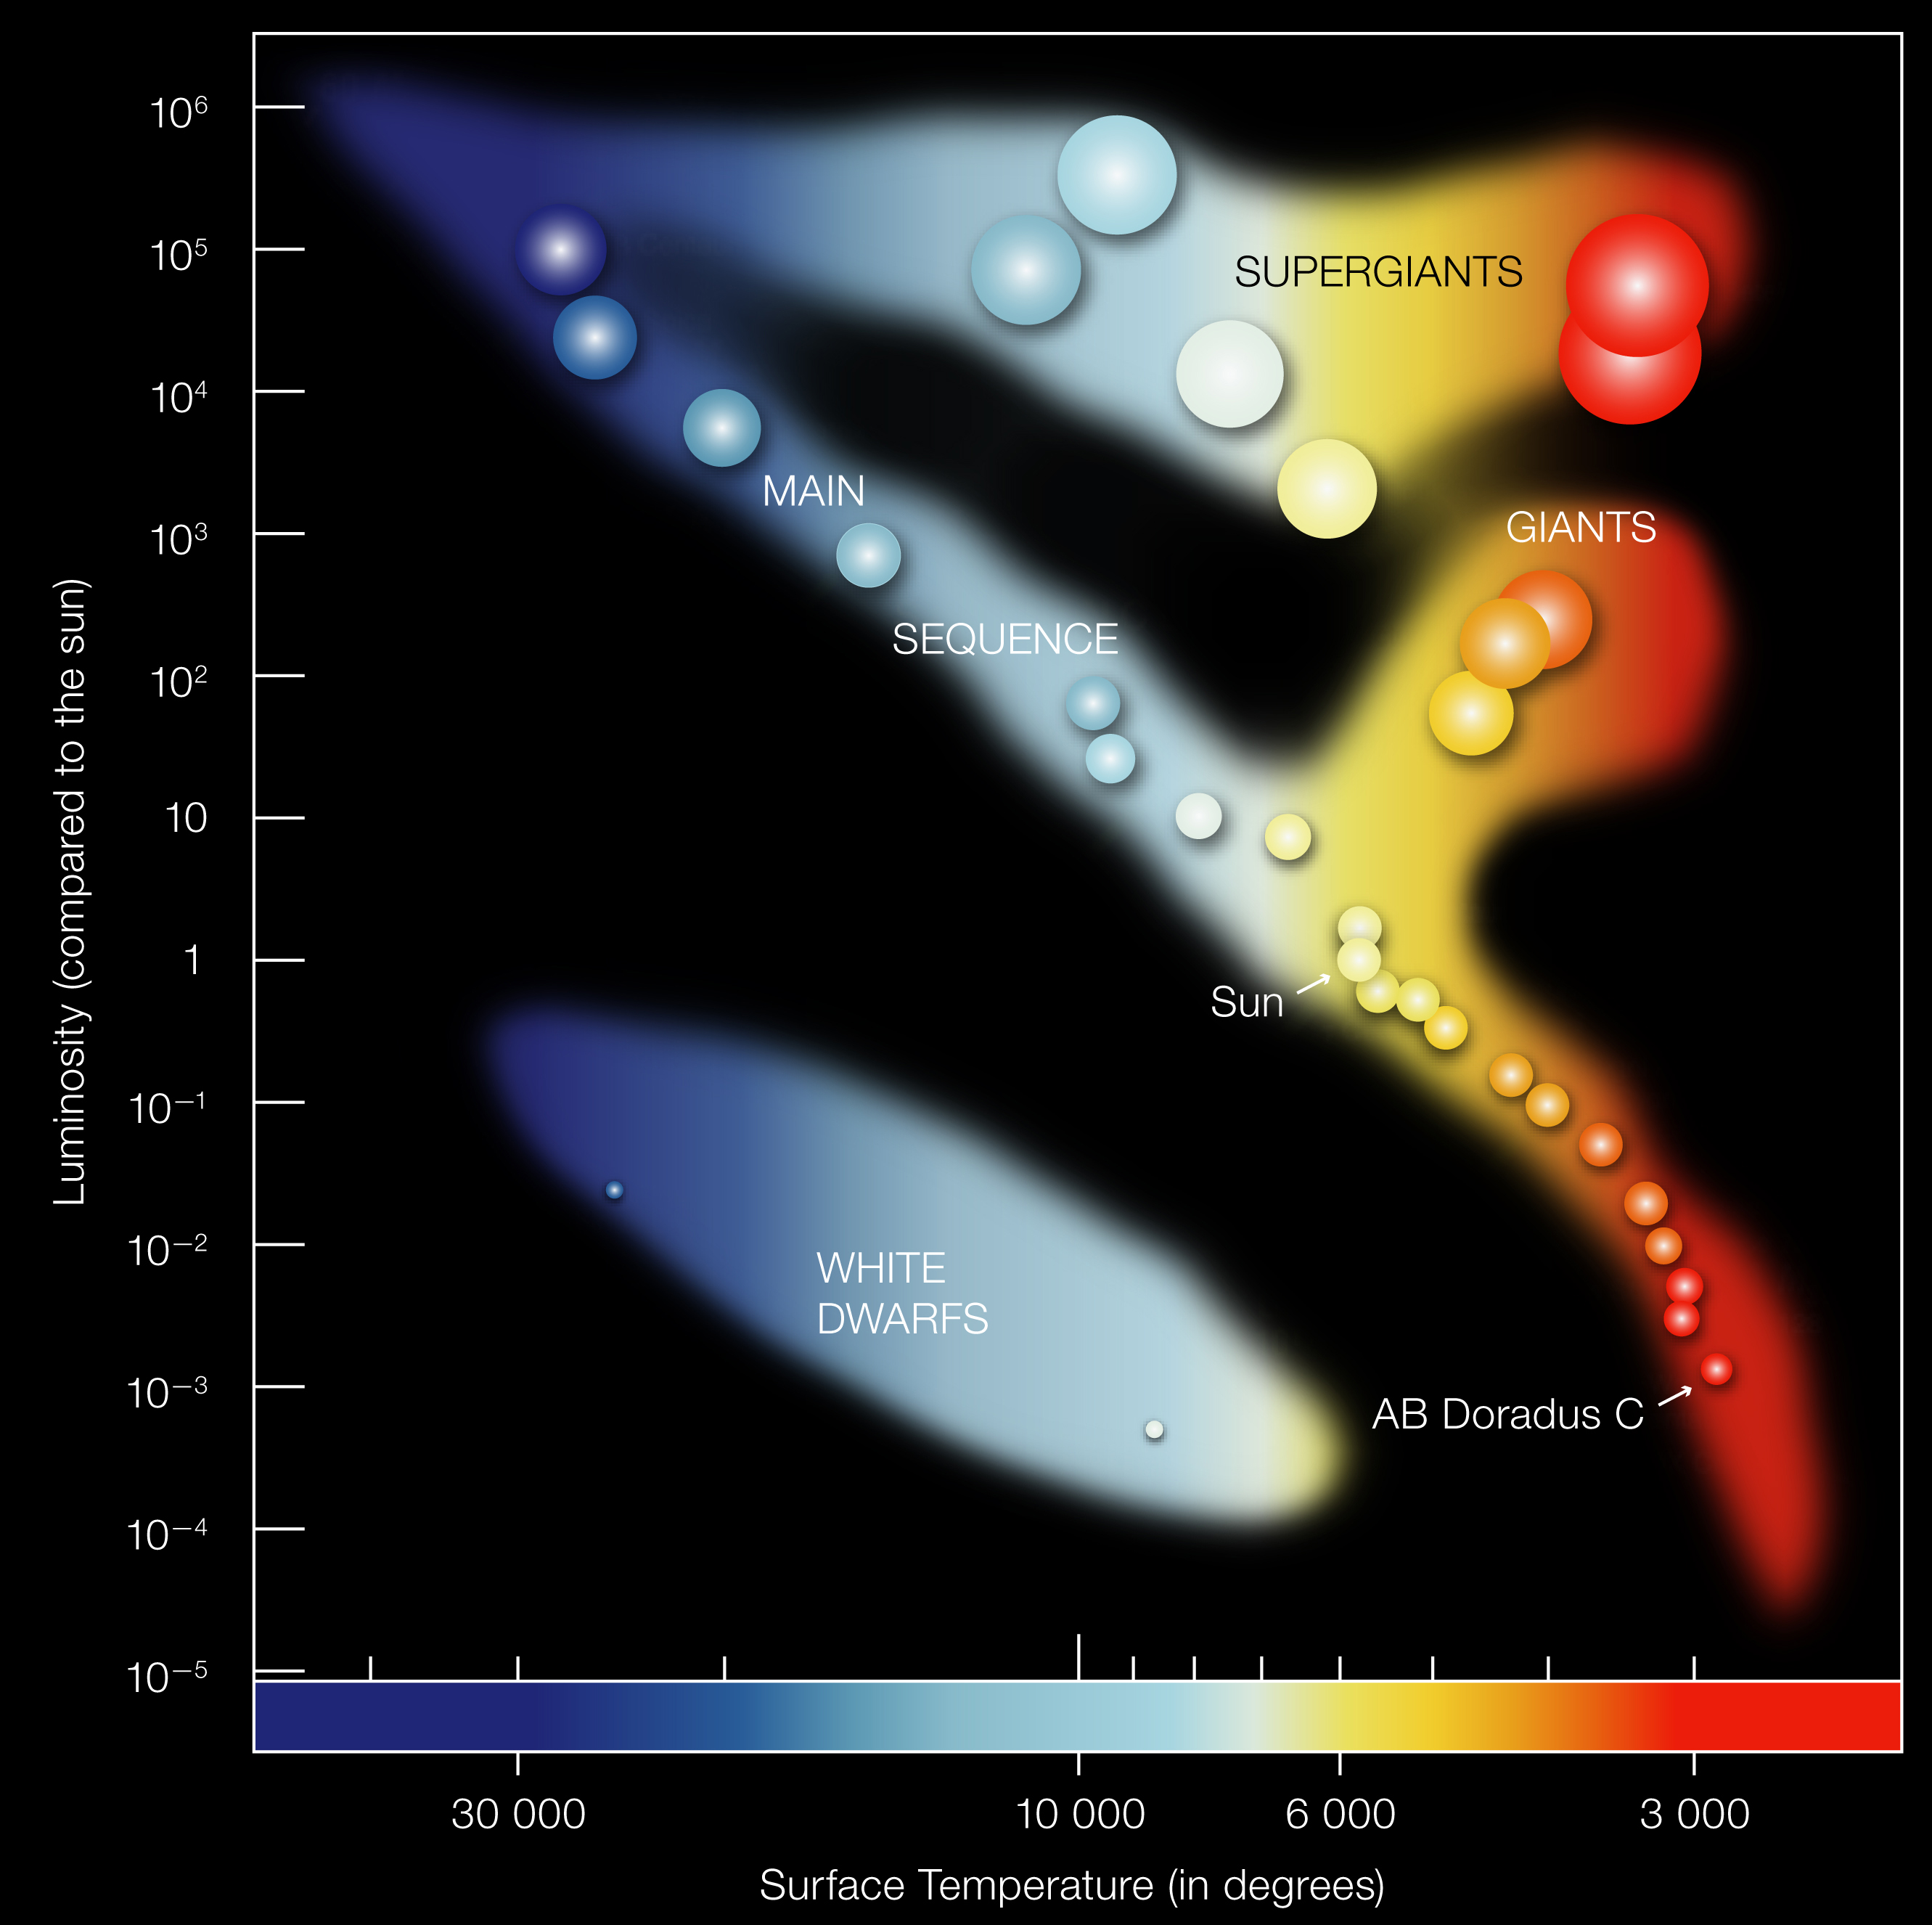
\includegraphics[width=0.82\textwidth]{diagrama_hr_eso.png}
\caption{\textbf{Diagrama Hertzsprung-Russell.} Luminosidade (em unidades solares) contra temperatura efetiva, com o eixo de temperatura crescendo para a esquerda. A faixa diagonal é a sequência principal (\textit{main sequence}); acima e à direita estão gigantes (\textit{giants}) e supergigantes (\textit{supergiants}), frias mas luminosas por terem raios enormes; abaixo e à esquerda estão as anãs brancas (\textit{white dwarfs}), quentes mas pouco luminosas por terem raios pequenos. O tamanho dos círculos indica o raio relativo das estrelas. A posição de uma estrela combina temperatura, luminosidade, raio e estágio evolutivo. Crédito: ESO, licença CC BY 4.0 (eso0728c).}
\end{figure}

\aberturabloco{Estrelas}{Este capítulo conecta espectros, luminosidades, massas e modelos internos em uma leitura física do diagrama HR.}{Ao estudar estrelas, mantenha sempre quatro grandezas em diálogo: $M$, $R$, $L$ e $T_{\rm eff}$. Quase toda interpretação estelar move uma delas e observa a resposta das outras.}

O diagrama HR é bonito, mas seu valor real é quantitativo. A relação
\[
L=4\pi R^2\sigma T_{\rm eff}^4
\]
permite transformar posição no HR em uma estimativa de raio. Duas estrelas com a mesma temperatura, mas luminosidades diferentes, têm raios diferentes. Uma gigante vermelha pode ser fria e luminosa porque seu raio é enorme; uma anã branca pode ser quente e fraca porque seu raio é pequeno.

Para estudantes de Física, o passo seguinte é perceber que a sequência principal é uma família de soluções de equilíbrio. A estrela precisa satisfazer conservação de massa, equilíbrio hidrostático, transporte de energia e geração de energia. Em forma conceitual:
\[
\frac{dP}{dr}=-\frac{Gm\rho}{r^2},\qquad
\frac{dm}{dr}=4\pi r^2\rho,\qquad
\frac{dL}{dr}=4\pi r^2\rho\epsilon.
\]
Mesmo sem resolver numericamente essas equações, elas ensinam como pensar. Se a massa aumenta, a pressão central necessária aumenta; a temperatura central tende a subir; a taxa de fusão cresce; a luminosidade aumenta fortemente; o tempo de vida diminui.

\begin{figure}[htbp]
\centering
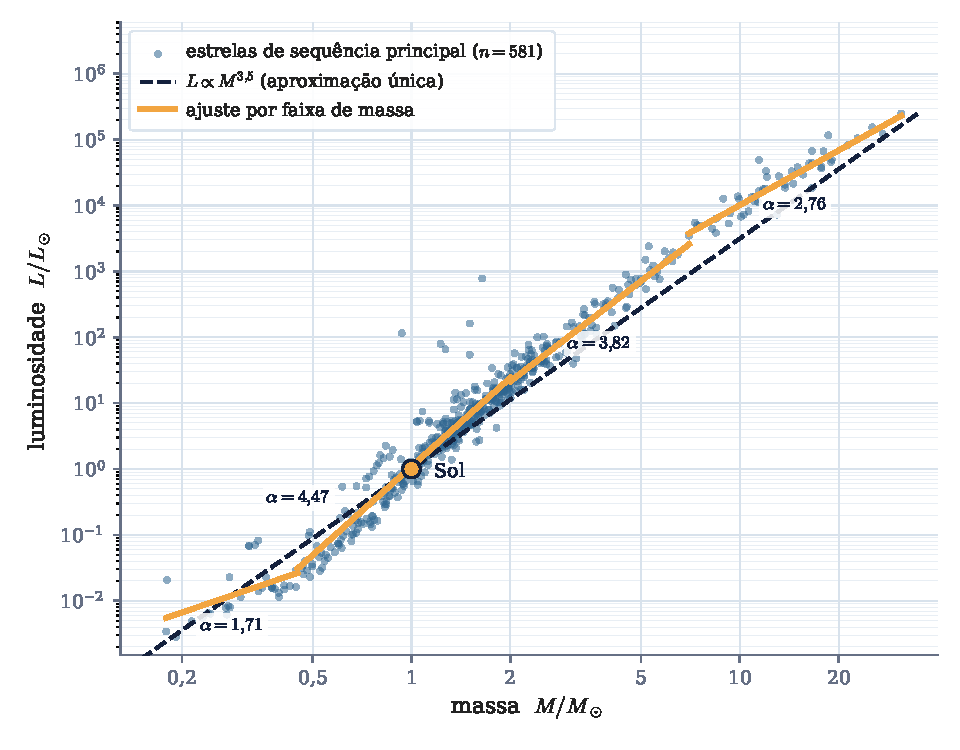
\includegraphics[width=0.88\textwidth]{relacao_massa_luminosidade.pdf}
\caption{\textbf{Relação massa-luminosidade da sequência principal.} Cada ponto é uma componente de binária eclipsante destacada com massa e raio medidos diretamente; a luminosidade vem de $L=4\pi R^2\sigma T_{\rm eff}^4$. Em escala log-log a relação é quase uma reta, o que significa uma lei de potência $L\propto M^\alpha$: pequenas mudanças de massa produzem grandes mudanças de luminosidade e, portanto, de tempo de vida. O expoente único $\alpha=3{,}5$ (tracejado) é uma boa aproximação de trabalho, mas o ajuste por faixas mostra que $\alpha$ varia de $\sim\!1{,}7$ nas anãs vermelhas a $\sim\!4{,}5$ perto da massa solar e volta a cair nas estrelas mais massivas, onde a pressão de radiação domina. Dados: Eker et al. (2018), MNRAS 479, 5491 (via VizieR).}
\end{figure}

\observaveis{classe espectral, magnitude, cor, paralaxe}{temperatura efetiva, luminosidade, raio, estágio evolutivo}{calibração fotométrica, correção de extinção, modelo atmosférico, distância confiável}{A posição no HR foi medida diretamente ou construída a partir de várias inferências?}

\textbf{Exemplo resolvido.} Considere uma estrela de sequência principal com $M=2M_\odot$ e use $L\propto M^{3{,}5}$. Então $L\simeq2^{3{,}5}L_\odot\simeq11L_\odot$. Se o combustível disponível cresce aproximadamente com $M$, mas o consumo cresce com $L$, o tempo de vida relativo escala como $t\propto M/L$. Assim, $t\simeq2/11\simeq0{,}18$ do tempo solar. Uma estrela mais massiva vive menos não por ter pouco combustível, mas por gastá-lo muito mais rápido.

\textbf{O que expandir no estudo individual.} Leia no Carroll \& Ostlie os trechos sobre equações de estrutura, opacidade e modelos estelares como um conjunto. Não tente memorizar cada fórmula isoladamente. Monte uma tabela com: equação, grandeza conservada, hipótese física e consequência observacional.

\begin{lessonblock}[borderline west={2pt}{0pt}{astroGold}]{Dedução curta: tempo de Kelvin-Helmholtz}
Antes de se compreender a fusão nuclear, uma hipótese natural era que estrelas brilhassem por contração gravitacional. A energia gravitacional disponível tem ordem
\[
E_g\sim\frac{GM^2}{R}.
\]
Dividindo pela luminosidade, obtemos uma escala de tempo:
\[
t_{\rm KH}\sim\frac{GM^2}{RL}.
\]
Para o Sol, isso dá dezenas de milhões de anos, muito menos que a idade geológica da Terra e que a idade solar conhecida. A discrepância histórica foi uma pista decisiva: a fonte de energia das estrelas precisava ser nuclear, não apenas gravitacional.
\end{lessonblock}

\begin{lessonblock}{Exemplo de aplicação: ponto de saída de aglomerados}
Em um aglomerado aberto, todas as estrelas nasceram aproximadamente juntas. Se o ponto de saída da sequência principal está perto de $M\simeq3M_\odot$, e se usamos $t\propto M/L$ com $L\propto M^{3{,}5}$, então
\[
t\propto M^{-2{,}5}.
\]
Comparado ao Sol, $t\simeq10\,\mathrm{Gyr}\times3^{-2{,}5}\simeq0{,}6\,\mathrm{Gyr}$. A idade estimada é grosseira, mas mostra por que o diagrama HR de um aglomerado funciona como relógio estelar.
\end{lessonblock}
\subsection*{Como a estrela decide qual reação usar}

A cadeia próton-próton e o ciclo CNO produzem o mesmo resultado líquido --- quatro prótons viram um núcleo de hélio, com liberação de $26{,}7\,\mathrm{MeV}$ --- mas dependem da temperatura de maneiras muito diferentes. Perto de $T\simeq1{,}5\times10^{7}\,\mathrm{K}$, a taxa da cadeia pp varia aproximadamente como $T^{4}$, enquanto a do ciclo CNO varia como $T^{17}$ ou mais. Essa diferença de expoente decide a arquitetura interna da estrela.

Em uma estrela de baixa massa, com núcleo relativamente frio, a cadeia pp domina e a produção de energia é distribuída em uma região ampla, o que favorece transporte radiativo no núcleo e convecção no envelope. Em uma estrela massiva, o CNO domina, e uma dependência $T^{17}$ concentra brutalmente a geração de energia no centro: o gradiente de temperatura necessário fica tão íngreme que a radiação não dá conta, e o núcleo torna-se convectivo. Duas estrelas da mesma família, portanto, têm estruturas internas invertidas --- e isso não é detalhe: núcleo convectivo significa combustível continuamente misturado, o que altera o tempo de vida e o caminho evolutivo.

\begin{lessonblock}[borderline west={2pt}{0pt}{astroGold}]{Dedução curta: por que estrelas massivas vivem tão pouco}
O combustível disponível é proporcional à massa, $E\propto M$, e a taxa de consumo é a luminosidade, $L$. O tempo de vida na sequência principal escala como
\[
t\propto\frac{M}{L}.
\]
Usando a relação massa-luminosidade da Figura~5, $L\propto M^{3{,}5}$ na faixa em torno da massa solar,
\[
t\propto M^{-2{,}5}.
\]
Com $t_\odot\simeq10^{10}$ anos, uma estrela de $10\,M_\odot$ vive $10^{10}\times10^{-2{,}5}\simeq3\times10^{7}$ anos, e uma de $0{,}5\,M_\odot$ viveria $\sim6\times10^{10}$ anos --- mais que a idade do universo, razão pela qual nenhuma anã vermelha jamais morreu por esgotamento de hidrogênio.

Essa única conta organiza boa parte da astrofísica galáctica: estrelas massivas são raras \emph{e} efêmeras, então onde há estrelas O e B há formação estelar recente; anãs vermelhas se acumulam desde sempre e dominam o inventário numérico da Galáxia.
\end{lessonblock}

\subsection*{Opacidade: o que segura o fóton}

O transporte radiativo depende de quão difícil é para um fóton atravessar o material, quantificado pela opacidade $\kappa$. Vários mecanismos competem: espalhamento por elétrons livres, que é praticamente independente do comprimento de onda e domina em plasmas muito quentes e ionizados; absorção livre-livre e ligado-livre, importantes em temperaturas intermediárias; e, em atmosferas frias como a solar, o íon negativo de hidrogênio $\mathrm{H^-}$, cuja presença é a principal razão pela qual o espectro do Sol tem a forma contínua que tem.

A opacidade entra na equação de transporte radiativo,
\[
\frac{dT}{dr}=-\frac{3\kappa\rho}{4ac T^{3}}\frac{L(r)}{4\pi r^{2}},
\]
que diz o seguinte em linguagem simples: quanto mais opaco o material e maior o fluxo que precisa atravessá-lo, mais íngreme tem de ser o gradiente de temperatura. Quando o gradiente exigido supera o gradiente adiabático, o material se torna instável e começa a convectar --- este é o critério de Schwarzschild, e é ele que determina onde estão as zonas convectivas de uma estrela.

\subsection*{Modelos estelares e o teorema de Vogt-Russell}

Juntando conservação de massa, equilíbrio hidrostático, transporte de energia e geração de energia, mais uma equação de estado e uma tabela de opacidades, obtém-se um sistema fechado. O enunciado clássico, conhecido como teorema de Vogt-Russell, afirma que massa e composição química determinam essencialmente a estrutura e a evolução de uma estrela. Ele não é um teorema no sentido matemático estrito --- rotação, campos magnéticos, perda de massa e binariedade quebram a unicidade ---, mas como princípio organizador é notavelmente eficaz: explica por que a sequência principal é uma linha e não uma nuvem.

\subsection*{O Sol como caso de teste}

O Sol é a única estrela cujo interior podemos sondar de duas maneiras independentes.

A primeira é a \textbf{heliossismologia}. A superfície solar oscila em milhões de modos acústicos superpostos, com períodos em torno de cinco minutos. Cada modo penetra até uma profundidade diferente, então o conjunto de frequências carrega informação sobre o perfil de velocidade do som --- e portanto de temperatura, densidade e composição --- em função do raio. A concordância entre os modelos e as frequências medidas chega a frações de por cento. É a melhor validação existente da teoria de estrutura estelar.

A segunda são os \textbf{neutrinos solares}. As reações nucleares produzem neutrinos que escapam praticamente sem interagir, entregando informação em tempo real do núcleo, ao contrário dos fótons, que levam dezenas de milhares de anos para difundir até a superfície. Durante décadas, os experimentos detectaram cerca de um terço do fluxo previsto, e a discrepância --- o ``problema dos neutrinos solares'' --- foi um dos casos mais instrutivos da física do século XX. A tentação era corrigir o modelo solar. A resposta, confirmada pelo observatório SNO no início dos anos 2000, veio da física de partículas: neutrinos oscilam entre sabores, e os detectores viam só um deles. O modelo estelar estava certo; a física de partículas é que estava incompleta.

Guarde esse episódio: quando dados e teoria discordam, o erro nem sempre está do lado em que se procura primeiro.

\subsection*{Sismologia estelar além do Sol}

A técnica que funcionou no Sol foi estendida a outras estrelas pelos telescópios espaciais Kepler e TESS, que medem brilho com precisão de partes por milhão e cadência de minutos. Milhares de gigantes vermelhas e estrelas de tipo solar têm hoje espectros de oscilação medidos, dos quais se extraem massa, raio e --- o mais valioso --- idade, com incerteza tipicamente de $10$ a $20\%$. Idades estelares eram, até pouco tempo atrás, a grandeza mais mal determinada da astrofísica estelar; a sismologia mudou isso e, de quebra, permitiu datar populações inteiras do disco e do halo galáctico.

\begin{lessonblock}{Exemplo de aplicação: idade de um aglomerado pelo ponto de desvio}
Todas as estrelas de um aglomerado nasceram praticamente juntas, da mesma nuvem. Como estrelas mais massivas evoluem mais rápido, elas deixam a sequência principal antes. O resultado, no diagrama HR do aglomerado, é um ``ponto de desvio'' (\textit{turnoff}): acima dele, a sequência principal está vazia.

A massa no ponto de desvio corresponde à massa cuja vida na sequência principal é igual à idade do aglomerado. Usando $t\simeq10^{10}(M/M_\odot)^{-2{,}5}$ anos, um aglomerado cujo desvio ocorre em $M\simeq2\,M_\odot$ tem idade
\[
t\simeq10^{10}\times2^{-2{,}5}\simeq1{,}8\times10^{9}\ \text{anos}.
\]
É por isso que uma única fotografia de um aglomerado, transformada em diagrama cor-magnitude, entrega uma idade. Com o Gaia fornecendo distâncias precisas para milhares de aglomerados, esse método virou uma cronologia da Via Láctea.
\end{lessonblock}

\textbf{Perguntas para discussão.}
\begin{itemize}
\item Por que uma dependência $T^{17}$ da taxa de reação produz núcleo convectivo, enquanto $T^{4}$ não?
\item O que a heliossismologia mede diretamente, e o que ela infere?
\item Se o problema dos neutrinos solares tivesse sido ``resolvido'' ajustando o modelo solar, que evidência posterior teria denunciado o erro?
\item Duas estrelas têm a mesma massa mas metalicidades diferentes. O que muda na estrutura?
\end{itemize}

\begin{lessonblock}[borderline west={2pt}{0pt}{astroGold}]{Laboratório de dados 4 -- a relação massa-luminosidade com estrelas reais}
\textbf{Arquivo:} \texttt{05\_estrelas\_massa\_raio\_teff.csv} --- 581 componentes de binárias eclipsantes destacadas, com massa, raio e temperatura efetiva medidos diretamente.

\textbf{Física.} A luminosidade sai da geometria mais Stefan-Boltzmann, e a relação massa-luminosidade sai do gráfico:
\[
\frac{L}{L_\odot}=\left(\frac{R}{R_\odot}\right)^{2}\left(\frac{T_{\rm ef}}{5772\,\mathrm{K}}\right)^{4},
\qquad
L\propto M^{\alpha}.
\]

\textbf{Roteiro.}
\begin{enumerate}
\item Calcule $L/L_\odot$ para cada estrela. No Excel: \texttt{=D2\^{}2*(E2/5772)\^{}4}.
\item Faça o gráfico de $\log_{10}L$ contra $\log_{10}M$. Ajuste uma reta e leia a inclinação: ela é o expoente $\alpha$.
\item Repita o ajuste separadamente para $M<2\,M_\odot$ e para $M>2\,M_\odot$. O expoente é o mesmo?
\item Estime o tempo de vida na sequência principal com $t\simeq10^{10}\,(M/L)$ anos, usando $M$ e $L$ em unidades solares. Faça o gráfico de $\log t$ contra $\log M$.
\end{enumerate}

\textbf{Entrega.} O diagrama massa-luminosidade com o ajuste, o valor de $\alpha$ em cada faixa e o tempo de vida estimado para uma estrela de $10\,M_\odot$ e para uma de $0{,}5\,M_\odot$.

\textbf{Confira.} Você deve encontrar $\alpha\simeq4{,}5$ perto da massa solar e $\alpha\simeq3{,}8$ acima de $2\,M_\odot$ --- compare com a Figura~5, que foi feita com este mesmo arquivo.
\end{lessonblock}

\newpage
\section*{Capítulo 6 -- Meio interestelar, formação e evolução estelar}
\addcontentsline{toc}{section}{Capítulo 6 -- Meio interestelar, formação e evolução estelar}
\imagemastro{0.86}{carina_nebula.jpg}{Região de formação estelar}{Nuvens de gás e poeira na Nebulosa de Carina mostram o ambiente onde novas estrelas nascem e interagem com radiação intensa. Crédito: NASA, ESA, N. Smith e Hubble Heritage Team, via Wikimedia Commons.}

A massa é o parâmetro dominante da evolução estelar. Uma estrela mais massiva tem mais combustível, mas consome esse combustível de forma muito mais rápida. Por isso vive menos. Uma estrela de baixa massa pode permanecer na sequência principal por dezenas ou centenas de bilhões de anos; uma estrela massiva pode evoluir em poucos milhões de anos. Essa diferença transforma aglomerados estelares em relógios: estrelas nascidas quase ao mesmo tempo, mas com massas diferentes, deixam a sequência principal em momentos diferentes. O ponto de saída fornece estimativas de idade.

Quando o hidrogênio central se esgota, a estrela precisa se reajustar. O núcleo contrai, camadas externas podem expandir e a estrela pode tornar-se gigante. Em massas adequadas, inicia-se queima de hélio em carbono e oxigênio. Estrelas de baixa e massa intermediária terminam como anãs brancas após perda de massa e formação de nebulosas planetárias. Estrelas massivas avançam por estágios sucessivos de fusão até formar núcleos ricos em ferro. Como fusão de ferro não libera energia em condições estelares usuais, o núcleo perde sustentação e pode colapsar, originando supernova e remanescente compacto.

Remanescentes compactos mostram regimes extremos da matéria. Anãs brancas são sustentadas por pressão de degenerescência dos elétrons. Estrelas de nêutrons envolvem densidades nucleares, campos magnéticos intensos e rotação rápida. Buracos negros aparecem quando nenhuma pressão conhecida impede a formação de um horizonte de eventos. Esses objetos conectam astrofísica estelar, relatividade, física nuclear e observações de altas energias. Eles também enriquecem a Galáxia: supernovas e ventos estelares devolvem elementos ao meio interestelar, preparando material para novas gerações de estrelas e planetas.

\textbf{Exemplo guiado.} Se duas estrelas têm a mesma temperatura efetiva, mas uma é 100 vezes mais luminosa, a relação $L=4\pi R^2\sigma T^4$ indica que a luminosidade cresce com $R^2$ quando $T$ é igual. Logo, a estrela mais luminosa tem raio 10 vezes maior. Esse raciocínio simples explica por que gigantes podem ser tão brilhantes mesmo com temperaturas superficiais relativamente baixas.

\textbf{Perguntas para discussão.}
\begin{itemize}
\item Por que massa inicial organiza tanto a vida de uma estrela?
\item Como o HR permite distinguir temperatura, luminosidade e tamanho?
\item O que significa uma estrela estar em equilíbrio se seu interior está em movimento?
\item Por que remanescentes compactos são laboratórios de física extrema?
\end{itemize}

\textbf{Para praticar.} Crie uma pequena lista de estrelas fictícias com temperatura, luminosidade e massa aproximada. Posicione cada estrela em um diagrama HR esquemático e proponha seu estágio evolutivo. Em seguida, considere incertezas como poeira, distância mal medida e binaridade. Essa segunda leitura é mais realista e mostra por que classificação astrofísica depende de várias linhas de evidência.

\begin{lessonblock}[borderline west={2pt}{0pt}{astroGold}]{Dedução curta: equilíbrio hidrostático}
Considere uma casca esférica de raio $r$, espessura $dr$, densidade $\rho$ e massa interna $m(r)$. A força gravitacional por unidade de volume é aproximadamente $\rho Gm(r)/r^2$, apontando para dentro. Para que a casca não acelere, a diferença de pressão entre a face interna e a externa precisa equilibrar esse peso:
\[
P(r)-P(r+dr)\simeq \rho\frac{Gm(r)}{r^2}dr.
\]
Dividindo por $dr$ e tomando o limite diferencial,
\[
\frac{dP}{dr}=-\frac{Gm(r)\rho(r)}{r^2}.
\]
O sinal negativo apenas registra que a pressão diminui quando caminhamos para fora. A equação é local: ela vale camada por camada, não apenas para a estrela inteira.
\end{lessonblock}

\begin{lessonblock}{Exemplo de aplicação: raio a partir de $L$ e $T$}
Use a forma relativa da lei de Stefan-Boltzmann:
\[
\frac{L}{L_\odot}=\left(\frac{R}{R_\odot}\right)^2\left(\frac{T}{T_\odot}\right)^4.
\]
Uma estrela gigante tem $L=100L_\odot$ e $T\simeq T_\odot/2$. Então
\[
100=\left(\frac{R}{R_\odot}\right)^2\left(\frac{1}{2}\right)^4
\]
e $R/R_\odot=\sqrt{1600}=40$. A estrela é fria na superfície, mas muito luminosa porque a área emissora é enorme. Esse é o tipo de leitura física que o diagrama HR deve provocar.
\end{lessonblock}

\subsection*{As fases do meio interestelar}

O gás entre as estrelas não é homogêneo; ele se organiza em fases com densidades e temperaturas que diferem por muitas ordens de grandeza, mas com pressões comparáveis --- o que faz sentido, já que fases em contato tendem ao equilíbrio de pressão, não de temperatura.

\begin{lessonblock}{Fases do meio interestelar}
\begin{tabular}{>{\raggedright\arraybackslash}p{0.26\textwidth}>{\raggedright\arraybackslash}p{0.15\textwidth}>{\raggedright\arraybackslash}p{0.15\textwidth}>{\raggedright\arraybackslash}p{0.30\textwidth}}
\toprule
Fase & $T$ (K) & $n$ (cm$^{-3}$) & Como é observada \\
\midrule
Nuvens moleculares & $10$--$50$ & $10^{2}$--$10^{6}$ & CO em rádio/mm, poeira em submm \\
Gás neutro frio & $\sim100$ & $\sim30$ & Linha de $21\,\mathrm{cm}$ em absorção \\
Gás neutro morno & $\sim8000$ & $\sim0{,}3$ & Linha de $21\,\mathrm{cm}$ em emissão \\
Gás ionizado morno & $\sim10^{4}$ & $0{,}1$--$10^{4}$ & Linhas de recombinação, H$\alpha$ \\
Gás coronal quente & $\sim10^{6}$ & $\sim10^{-3}$ & Raios X moles, absorção no UV \\
\bottomrule
\end{tabular}
\end{lessonblock}

A poeira representa cerca de $1\%$ da massa do gás, mas domina a aparência: grãos de silicato e carbono com tamanhos de décimos de micrômetro espalham luz azul com muito mais eficiência que vermelha. Daí a extinção seletiva --- objetos atrás de poeira parecem mais fracos \emph{e} mais vermelhos ---, quantificada pelo excesso de cor $E(B-V)$ e pela razão $R_V=A_V/E(B-V)$, tipicamente próxima de $3{,}1$ na Galáxia. Confundir avermelhamento por poeira com temperatura baixa intrínseca é um dos erros clássicos da área, e é por isso que estimativas de temperatura por cor precisam sempre ser corrigidas por extinção.

Os grãos não são apenas obstáculo. Eles são superfície de catálise --- é neles que o hidrogênio molecular se forma --- e são refrigerantes: absorvem luz estelar ultravioleta e reemitem no infravermelho distante, retirando energia da nuvem e permitindo que ela esfrie o suficiente para colapsar.

\begin{lessonblock}[borderline west={2pt}{0pt}{astroGold}]{Dedução curta: o critério de Jeans}
Uma nuvem colapsa quando a gravidade vence a pressão térmica. Comparando as duas energias para uma esfera de massa $M$, raio $R$, temperatura $T$ e massa média por partícula $\mu m_H$:
\[
|E_{\rm grav}|\sim\frac{GM^{2}}{R},\qquad E_{\rm term}\sim\frac{3}{2}\frac{M}{\mu m_H}kT.
\]
Impondo $|E_{\rm grav}|>2E_{\rm term}$ (teorema do virial) e eliminando $R$ em favor da densidade, obtém-se a massa mínima para colapso:
\[
M_J\simeq\left(\frac{5kT}{G\mu m_H}\right)^{3/2}\left(\frac{3}{4\pi\rho}\right)^{1/2}.
\]
O que importa é a dependência: $M_J\propto T^{3/2}\rho^{-1/2}$. Gás frio e denso colapsa facilmente; gás quente e rarefeito, não. Para uma nuvem molecular típica, com $T\simeq10\,\mathrm{K}$ e $n\simeq10^{4}\,\mathrm{cm^{-3}}$, a massa de Jeans é de poucas massas solares --- e é por isso que nuvens moleculares gigantes, com $10^{5}\,M_\odot$, não formam uma estrela gigantesca, e sim milhares de estrelas: elas se fragmentam, porque cada sub-região já excede sua própria massa de Jeans local.
\end{lessonblock}

\subsection*{Do colapso ao disco}

O colapso não é uma queda livre limpa. Duas grandezas conservadas atrapalham: momento angular e fluxo magnético. Uma nuvem com rotação lentíssima, ao encolher por várias ordens de grandeza em raio, gira rápido demais para colapsar diretamente --- e por isso o material se organiza em um \textbf{disco de acreção}, que redistribui momento angular para fora enquanto a massa cai para dentro. É essa geometria imposta pela física de rotação que torna discos protoplanetários uma consequência necessária, e não um acidente, da formação estelar.

A protoestrela em formação também expele material em jatos colimados ao longo do eixo de rotação, visíveis como objetos Herbig-Haro. Esse feedback --- junto com a radiação ultravioleta e os ventos das estrelas mais massivas recém-formadas --- limita a eficiência do processo: apenas alguns por cento da massa de uma nuvem molecular vira estrela antes que ela seja dispersada.

O ALMA transformou esse assunto ao produzir imagens diretas de discos protoplanetários com resolução de dezenas de milissegundos de arco, revelando anéis, lacunas e espirais que provavelmente marcam a presença de planetas em formação. O JWST complementou olhando a química: gelo, água e moléculas orgânicas nas regiões internas dos mesmos discos. A formação planetária deixou de ser inferida a partir do resultado final e passou a ser observada em andamento.

\subsection*{A função de massa inicial}

Nem todas as massas são igualmente prováveis. A distribuição de massas com que as estrelas nascem, a função de massa inicial (IMF), é aproximadamente uma lei de potência para massas acima de uma massa solar,
\[
\frac{dN}{dM}\propto M^{-2{,}35},
\]
a forma de Salpeter, achatando-se abaixo disso. A consequência quantitativa é forte: para cada estrela de $20\,M_\odot$ nascem centenas de estrelas de tipo solar e milhares de anãs vermelhas. Massa, porém, não é luminosidade --- as poucas estrelas massivas dominam a luz emitida e a produção de elementos pesados, enquanto as anãs dominam a contagem e a massa estelar total. Quase toda inferência sobre populações estelares distantes depende de assumir uma IMF, e essa é uma das hipóteses mais frequentemente citadas quando resultados extragalácticos precisam ser revistos.

\subsection*{Depois da sequência principal}

Quando o hidrogênio central acaba, o núcleo de hélio inerte contrai e aquece, a queima passa a ocorrer em uma camada em torno dele, e o envelope se expande enormemente: a estrela vira gigante vermelha. Em estrelas de massa intermediária, segue-se a queima de hélio em carbono e oxigênio pelo processo triplo-alfa, iniciada de forma explosiva (o \textit{flash} do hélio) quando o núcleo está degenerado.

Na fase final, no ramo assintótico das gigantes, duas camadas queimam alternadamente em pulsos térmicos, e a convecção profunda draga para a superfície elementos recém-sintetizados --- é ali que se produz boa parte do carbono e dos elementos do processo $s$ do universo. A estrela então ejeta o envelope, formando uma nebulosa planetária, e o que resta do núcleo esfria como anã branca.

Estrelas acima de aproximadamente $8\,M_\odot$ seguem outro caminho: conseguem queimar carbono, néon, oxigênio e silício em camadas sucessivas, montando uma estrutura em cebola com um núcleo de ferro. Como o ferro é o ponto mais fundo da curva de energia de ligação nuclear, fundi-lo consome energia em vez de liberar. O núcleo perde suporte, colapsa em frações de segundo e a estrela explode como supernova de colapso de núcleo, deixando uma estrela de nêutrons ou um buraco negro.

\begin{lessonblock}{Exemplo de aplicação: de onde vêm os elementos}
Vale ter presente a divisão de trabalho da nucleossíntese, porque ela conecta capítulos distantes desta apostila:
\begin{itemize}
\item \textbf{Hidrogênio, hélio e um pouco de lítio}: nucleossíntese primordial, nos primeiros minutos (Capítulo 14).
\item \textbf{Carbono, nitrogênio, oxigênio}: queima em estrelas e dragagem em gigantes do ramo assintótico.
\item \textbf{Elementos até o ferro}: queima em camadas de estrelas massivas e supernovas de colapso de núcleo.
\item \textbf{Ferro em grande quantidade}: supernovas termonucleares de tipo Ia.
\item \textbf{Ouro, platina, lantanídeos e outros do processo $r$}: fusões de estrelas de nêutrons, confirmadas observacionalmente em GW170817 (Capítulo 8).
\end{itemize}
A frase feita de que ``somos poeira de estrelas'' tem, portanto, endereços diferentes para cada átomo --- e um deles só foi confirmado em 2017.
\end{lessonblock}

\textbf{Perguntas para discussão.}
\begin{itemize}
\item Por que nuvens moleculares gigantes formam milhares de estrelas em vez de uma só?
\item Que evidência observacional apoia a existência de discos em torno de estrelas jovens?
\item Se a IMF fosse diferente em galáxias distantes, que conclusões extragalácticas mudariam?
\item Por que a queima de ferro não sustenta uma estrela, mesmo com ferro em abundância no núcleo?
\end{itemize}

\newpage
\section*{Capítulo 7 -- Remanescentes compactos e altas energias}
\addcontentsline{toc}{section}{Capítulo 7 -- Remanescentes compactos e altas energias}
\aberturabloco{Altas energias}{O fio condutor deste capítulo é a pergunta: o que acontece quando a gravidade força a matéria para regimes em que pressão térmica comum não basta?}{Acompanhe sempre três escalas: densidade, velocidade de escape e tempo de variabilidade. Elas dizem se o objeto é comum, compacto ou extremo.}

Anãs brancas, estrelas de nêutrons e buracos negros são finais possíveis de evolução estelar, mas também são laboratórios de Física. Em uma anã branca, a sustentação vem da pressão de degenerescência dos elétrons. Em uma estrela de nêutrons, densidades nucleares tornam a equação de estado um problema profundo. Em buracos negros, o horizonte de eventos marca uma fronteira causal.

A escala relativística mais simples é o raio de Schwarzschild:
\[
R_s=\frac{2GM}{c^2}.
\]
Para uma massa solar, $R_s\simeq3\,\mathrm{km}$. Essa aproximação é uma âncora útil: um buraco negro de $10M_\odot$ tem raio de Schwarzschild de ordem $30\,\mathrm{km}$; um buraco negro supermassivo de $4\times10^6M_\odot$ tem escala de milhões de quilômetros.

\begin{figure}[htbp]
\centering
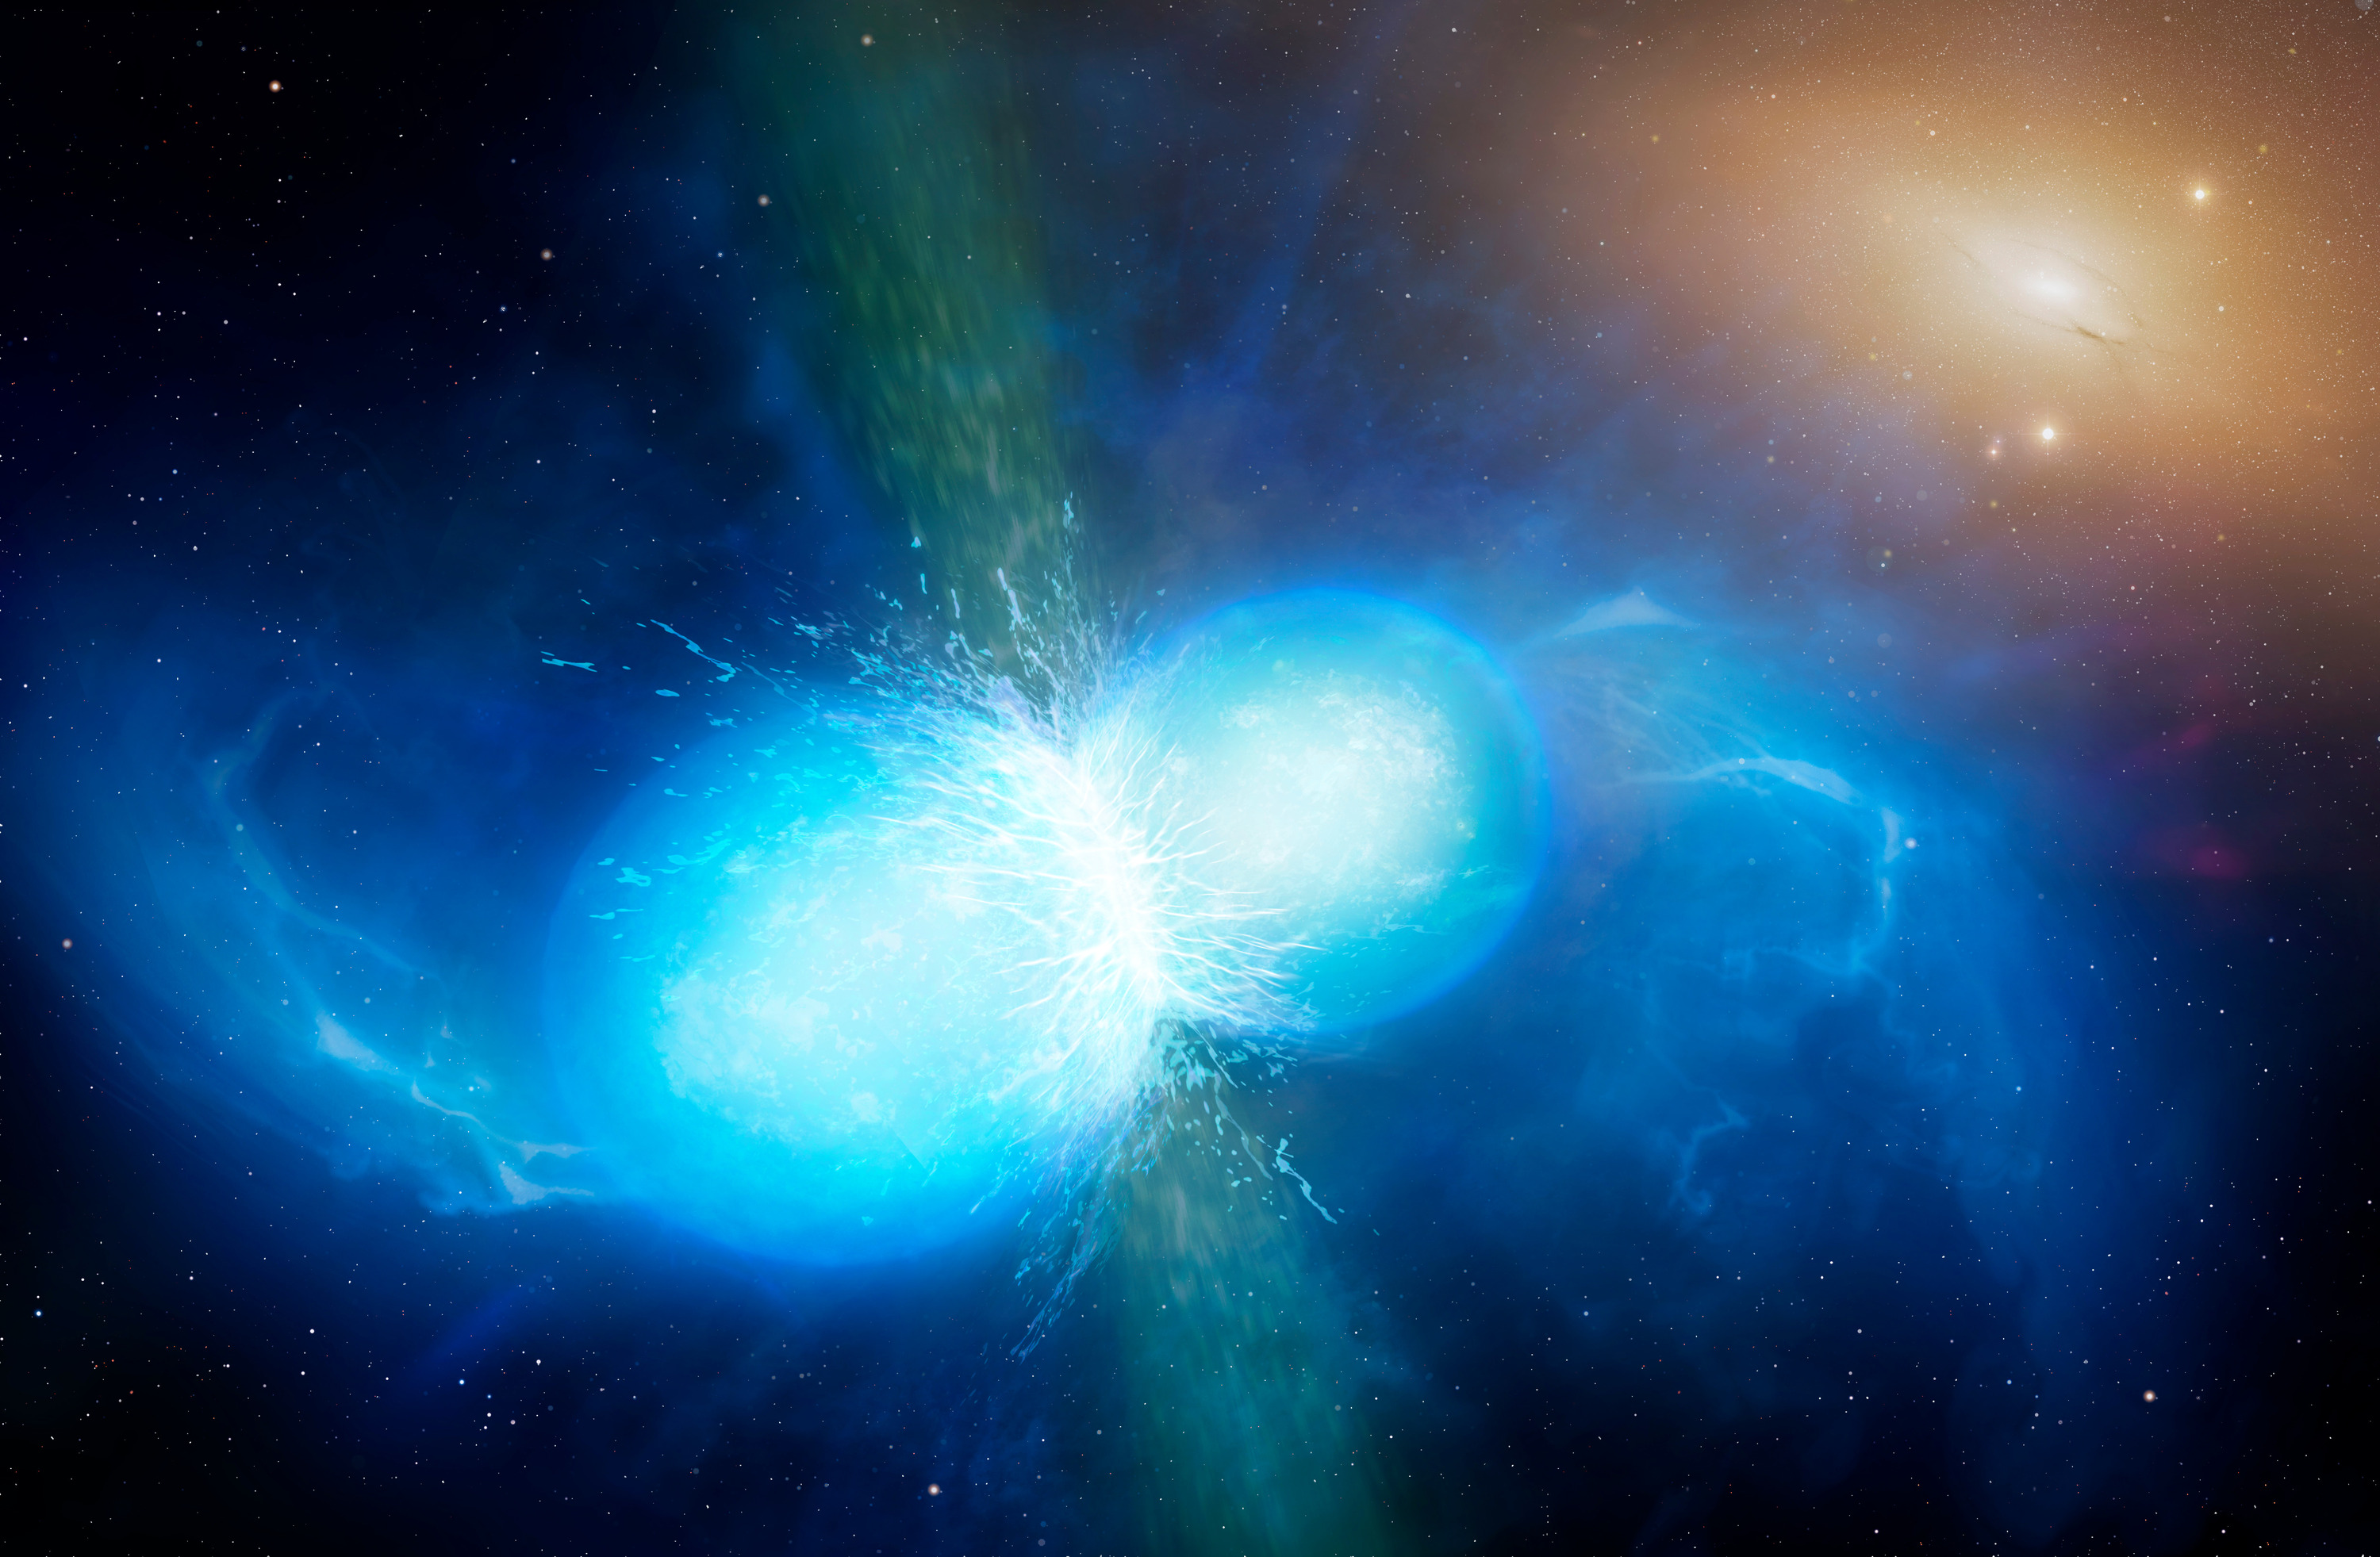
\includegraphics[width=\textwidth]{fusao_estrelas_neutrons.jpg}
\caption{\textbf{O regime compacto em ação: fusão de duas estrelas de nêutrons.} Concepção artística do evento GW170817, detectado em 17 de agosto de 2017 simultaneamente em ondas gravitacionais (LIGO--Virgo) e em raios gama (Fermi/INTEGRAL), e depois acompanhado em todo o espectro eletromagnético. Cada uma das duas estrelas concentra mais de uma massa solar em um raio de cerca de $10\,\mathrm{km}$: a mesma massa do Sol comprimida do tamanho de uma cidade. É essa compactação extrema --- de $R\sim R_\oplus$ nas anãs brancas, a $R\sim10\,\mathrm{km}$ nas estrelas de nêutrons, até $R_s=2GM/c^2\simeq3\,\mathrm{km}$ por massa solar no horizonte de um buraco negro --- que torna acessíveis densidades nucleares, campos gravitacionais relativísticos e a nucleossíntese de elementos pesados observada na quilonova. Crédito: University of Warwick/Mark Garlick, via ESO, licença CC BY 4.0 (eso1733s).}
\end{figure}

\observaveis{raios X, pulsos periódicos, variabilidade rápida, órbitas de companheiras}{massa compacta, raio máximo da região emissora, campo magnético, taxa de acreção}{modelo de emissão, inclinação orbital, distância, identificação do objeto companheiro}{A luminosidade vem da superfície, de um disco de acreção ou de uma região relativística?}

\textbf{Exemplo resolvido.} Se uma fonte varia significativamente em $\Delta t=1\,\mathrm{ms}$, a região que coordena essa variação não pode ter tamanho muito maior que $c\Delta t\approx3\times10^5\,\mathrm{m}=300\,\mathrm{km}$. Isso não prova sozinho que há uma estrela de nêutrons ou buraco negro, mas coloca a fonte no regime compacto. Variabilidade é uma régua causal.

\textbf{Conexão com supernovas.} Supernovas não são apenas explosões bonitas. Elas conectam nucleossíntese, ondas de choque, neutrinos, poeira, enriquecimento químico e formação de remanescentes. Ao estudar uma supernova, pergunte: que estrela explodiu? Qual fonte de energia alimentou a luz? Que elementos foram produzidos? Que remanescente sobrou?

\begin{lessonblock}[borderline west={2pt}{0pt}{astroGold}]{Dedução curta: raio de Schwarzschild por argumento de escape}
Uma forma newtoniana de motivar a escala de Schwarzschild é perguntar em que raio a velocidade de escape seria igual à velocidade da luz:
\[
v_{\rm esc}=\sqrt{\frac{2GM}{R}}=c.
\]
Daí,
\[
R=\frac{2GM}{c^2}.
\]
Relatividade geral é necessária para interpretar corretamente o horizonte, mas o argumento dimensional revela a escala certa. Para $M=M_\odot$, $R_s\simeq3\,\mathrm{km}$; para $10M_\odot$, $R_s\simeq30\,\mathrm{km}$.
\end{lessonblock}

\begin{lessonblock}{Exemplo de aplicação: luminosidade de acreção}
Uma massa $m$ caindo até raio $R$ libera energia gravitacional de ordem $GMm/R$. Por unidade de tempo, para uma taxa de acreção $\dot M$,
\[
L_{\rm acc}\sim\frac{GM\dot M}{R}.
\]
Como $R$ é pequeno em objetos compactos, a acreção pode ser muito eficiente. Essa é a razão física para discos de acreção em anãs brancas, estrelas de nêutrons e buracos negros brilharem em ultravioleta e raios X. A luz não vem de fusão nuclear comum, mas da conversão de energia gravitacional em radiação.
\end{lessonblock}
\subsection*{Anãs brancas e o limite de Chandrasekhar}

Uma anã branca não é sustentada por pressão térmica, e sim pela pressão de degenerescência dos elétrons --- uma consequência direta do princípio de exclusão de Pauli, que impede dois elétrons de ocuparem o mesmo estado quântico. O resultado é contraintuitivo: quanto \emph{maior} a massa, \emph{menor} o raio, porque a gravidade extra precisa ser equilibrada por elétrons empacotados mais densamente.

Levando o raciocínio ao limite, quando os elétrons se tornam relativísticos a pressão deixa de crescer rápido o bastante e existe uma massa máxima, o limite de Chandrasekhar, próximo de $1{,}4\,M_\odot$. Esse número não é um ajuste empírico: sai da combinação de mecânica quântica, relatividade especial e gravitação newtoniana. E ele tem consequência observacional imediata --- é o gatilho das supernovas de tipo Ia, que ocorrem quando uma anã branca em sistema binário se aproxima desse limite. A uniformidade relativa dessas explosões é o que as torna velas padrão e sustenta a medida da aceleração cósmica (Capítulo 13).

\subsection*{Pulsares: relógios naturais}

Estrelas de nêutrons magnetizadas e em rotação rápida emitem feixes que varrem o espaço; se o feixe cruza a Terra, vemos pulsos periódicos. Os pulsares mais rápidos, chamados de milissegundo, giram centenas de vezes por segundo e mantêm estabilidade de período comparável à de relógios atômicos.

Essa estabilidade é o que os torna instrumentos. O pulsar binário de Hulse e Taylor teve seu período orbital medido decrescendo exatamente na taxa prevista pela relatividade geral para perda de energia por ondas gravitacionais --- primeira evidência, ainda que indireta, dessas ondas, e Nobel de 1993. Conjuntos de pulsares espalhados pela Galáxia formam hoje detectores de ondas gravitacionais de baixíssima frequência (Capítulo 8), e o retardo dependente da frequência dos pulsos mede o plasma no caminho (Capítulo 15).

\textbf{Magnetares.} Uma subclasse tem campos magnéticos de $10^{14}$ a $10^{15}\,\mathrm{G}$, os mais intensos conhecidos no universo. Reconfigurações desses campos produzem surtos de raios X e gama, e pelo menos um magnetar galáctico já foi flagrado emitindo uma rápida rajada de rádio, conectando dois campos que pareciam separados.

\subsection*{Medindo o raio de uma estrela de nêutrons}

Massas de estrelas de nêutrons são medidas há décadas em sistemas binários, e alguns pulsares chegam a $\sim2\,M_\odot$ --- o que por si só descarta equações de estado nucleares que não suportariam tanto. O raio é bem mais difícil. Duas técnicas modernas atacaram o problema: o telescópio NICER, instalado na Estação Espacial Internacional, modela o perfil temporal e espectral de manchas quentes na superfície de pulsares, cuja forma depende da curvatura do espaço-tempo e portanto da razão massa-raio; e a deformabilidade de maré extraída da forma de onda de GW170817, que mede o quanto cada estrela é distorcida pela companheira antes da fusão.

As duas rotas, partindo de física completamente diferente, convergem para raios em torno de $12\,\mathrm{km}$ para estrelas de $1{,}4\,M_\odot$. É um resultado bonito de consistência: astrofísica de raios X e astronomia de ondas gravitacionais restringindo, juntas, a física nuclear de altíssima densidade.

\subsection*{Acreção, discos e jatos}

Em binárias próximas, matéria transferida de uma companheira forma um disco em torno do objeto compacto. A luminosidade de acreção é
\[
L_{\rm acc}\sim\frac{GM\dot{M}}{R},
\]
e a eficiência --- energia liberada por unidade de massa acretada --- vale aproximadamente $GM/Rc^{2}$. Para uma estrela de nêutrons, isso dá cerca de $10$ a $20\%$ de $mc^{2}$, quase uma ordem de grandeza acima da eficiência da fusão nuclear, que é de $0{,}7\%$. Acreção sobre objetos compactos é o processo mais eficiente de conversão de massa em energia conhecido na natureza, e é por isso que binárias de raios X e núcleos ativos brilham tanto com tão pouca matéria.

Há um teto natural: quando a pressão de radiação sobre o gás em queda iguala a atração gravitacional, a acreção se auto-limita. Essa é a \textbf{luminosidade de Eddington},
\[
L_{\rm Edd}=\frac{4\pi GMm_pc}{\sigma_T}\simeq1{,}3\times10^{31}\left(\frac{M}{M_\odot}\right)\,\mathrm{W},
\]
um número que reaparece em contextos muito distantes: limita o brilho de binárias de raios X, o crescimento de buracos negros supermassivos no universo jovem e a interpretação de fontes ultraluminosas.

\subsection*{Ver o horizonte: imagens e órbitas}

Duas linhas observacionais recentes tornaram buracos negros objetos de imagem, não só de inferência.

A primeira é o \textbf{Event Horizon Telescope}, que combinou radiotelescópios de vários continentes em $1{,}3\,\mathrm{mm}$ e produziu, em 2019, a imagem do anel de emissão em torno do buraco negro de M\,87, e em 2022 a de Sagitário A*, no centro da nossa Galáxia. O que se vê não é o horizonte --- ele é escuro por definição --- mas a sombra que ele projeta sobre o plasma quente ao redor, com tamanho previsto pela relatividade geral a partir da massa.

A segunda é o acompanhamento de \textbf{órbitas estelares individuais} no centro galáctico. Duas equipes seguiram por décadas, com óptica adaptativa, estrelas que orbitam Sagitário A* --- a estrela S2 completa uma volta em cerca de $16$ anos --- e mediram a massa central em torno de $4\times10^{6}\,M_\odot$ concentrada em uma região menor que o Sistema Solar. O trabalho rendeu metade do Nobel de Física de 2020 e forneceu testes diretos de relatividade geral: o avanço do periastro de S2 e o desvio gravitacional para o vermelho de sua luz na passagem mais próxima foram medidos e batem com a previsão.

\begin{lessonblock}{Exemplo resolvido: a sombra de Sagitário A*}
O raio de Schwarzschild de $4{,}3\times10^{6}\,M_\odot$ é
\[
R_s=\frac{2GM}{c^{2}}\simeq1{,}3\times10^{10}\,\mathrm{m}.
\]
A sombra prevista tem diâmetro angular de aproximadamente $5{,}2R_s$ dividido pela distância de $8{,}3\,\mathrm{kpc}=2{,}6\times10^{20}\,\mathrm{m}$:
\[
\theta\simeq\frac{5{,}2\times1{,}3\times10^{10}}{2{,}6\times10^{20}}\simeq2{,}6\times10^{-10}\,\mathrm{rad}\simeq54\ \mu\text{as}.
\]
Resolver isso em $1{,}3\,\mathrm{mm}$ exige, por $\theta\simeq\lambda/B$, uma linha de base
\[
B\simeq\frac{1{,}3\times10^{-3}}{2{,}6\times10^{-10}}\simeq5\times10^{6}\,\mathrm{m},
\]
ou seja, cinco mil quilômetros --- da ordem do raio da Terra. A conta explica em uma linha por que a imagem só foi possível com um interferômetro de escala planetária, e por que não havia atalho.
\end{lessonblock}

\textbf{Perguntas para discussão.}
\begin{itemize}
\item Por que o raio de uma anã branca diminui quando sua massa aumenta?
\item Acreção é mais eficiente que fusão nuclear. Por que, então, estrelas usam fusão?
\item O EHT fotografa a sombra, não o horizonte. Que diferença física há entre as duas coisas?
\item Que hipóteses entram ao converter o movimento de S2 em uma massa central?
\item Duas técnicas independentes dão raio $\simeq12\,\mathrm{km}$ para estrelas de nêutrons. Por que a concordância vale mais que qualquer uma delas isolada?
\end{itemize}

\begin{lessonblock}[borderline west={2pt}{0pt}{astroGold}]{Laboratório de dados 5 -- pulsares como laboratórios de rotação}
\textbf{Arquivo:} \texttt{07\_pulsares\_atnf.csv} --- 2052 pulsares reais com período $P$ e derivada $\dot{P}$ medidos.

\textbf{Física.} Um pulsar perde energia rotacional e desacelera. Com momento de inércia $I\simeq10^{38}\,\mathrm{kg\,m^{2}}$:
\[
\dot{E}=4\pi^{2}I\frac{\dot{P}}{P^{3}},\qquad
\tau=\frac{P}{2\dot{P}},\qquad
B_{\rm sup}\simeq3{,}2\times10^{19}\sqrt{P\dot{P}}\ \mathrm{G}.
\]
A primeira é a luminosidade de desaceleração, a segunda é a idade característica e a terceira estima o campo magnético na superfície.

\textbf{Roteiro.}
\begin{enumerate}
\item Calcule $\dot{E}$, $\tau$ e $B_{\rm sup}$ para todos os pulsares. Em Excel, três colunas de fórmula.
\item Construa o \textbf{diagrama $P$--$\dot{P}$}: $\log\dot{P}$ contra $\log P$. Este é o diagrama HR da astronomia de pulsares.
\item Marque as linhas de $B$ constante e de $\tau$ constante --- elas são retas neste diagrama. Deduza por quê.
\item Identifique os dois agrupamentos: pulsares jovens no alto e pulsares de milissegundo no canto inferior esquerdo. Compare idades características e campos magnéticos dos dois grupos.
\end{enumerate}

\textbf{Entrega.} O diagrama $P$--$\dot{P}$ anotado, os valores das três grandezas para o pulsar do Caranguejo ($P\simeq0{,}0334\,\mathrm{s}$) e uma discussão: por que pulsares de milissegundo têm idade característica de bilhões de anos e campo fraco?

\textbf{Confira.} Para o Caranguejo você deve obter $\dot{E}\sim4\times10^{31}\,\mathrm{W}$ e $\tau\sim1{,}2\times10^{3}$ anos --- a supernova que o gerou foi registrada por astrônomos chineses em 1054, ou seja, há cerca de mil anos.
\end{lessonblock}

\newpage
\section*{Capítulo 8 -- Ondas gravitacionais e astronomia multimensageira}
\addcontentsline{toc}{section}{Capítulo 8 -- Ondas gravitacionais e astronomia multimensageira}
Até 2015, toda a astronomia era feita com radiação eletromagnética, com duas exceções pontuais: raios cósmicos e um punhado de neutrinos da supernova SN\,1987A. Em 14 de setembro de 2015, os detectores LIGO registraram a passagem de uma onda gravitacional produzida pela fusão de dois buracos negros, e a área ganhou um canal de informação que não depende de fótons. Este capítulo trata desse canal e do que acontece quando ele é combinado com os demais.

\subsection*{O que é uma onda gravitacional}

Na relatividade geral, massa e energia curvam o espaço-tempo. Quando uma distribuição de massa se reorganiza de forma assimétrica e acelerada, essa curvatura se propaga como uma onda, à velocidade da luz. A onda não é uma perturbação \emph{no} espaço: ela é uma perturbação \emph{do} espaço. O efeito observável é que distâncias entre corpos livres oscilam. Se dois espelhos estão separados por $L$, a passagem de uma onda de amplitude $h$ produz
\[
\frac{\Delta L}{L}\simeq\frac{h}{2}.
\]
A grandeza $h$ é adimensional --- é uma deformação relativa, uma \textit{strain}. E é minúscula: para as fontes mais intensas já detectadas, $h\sim10^{-21}$.

Há uma diferença estrutural em relação ao eletromagnetismo que vale registrar. Não existe radiação gravitacional de dipolo, porque a conservação do momento a proíbe; a emissão mais baixa possível é de quadrupolo. Por isso um objeto perfeitamente esférico, mesmo colapsando, não emite ondas gravitacionais: é preciso assimetria. Uma estrela de nêutrons girando com uma montanha de poucos centímetros emite; a mesma estrela perfeitamente lisa, não.

\begin{lessonblock}[borderline west={2pt}{0pt}{astroGold}]{Dedução curta: por que só objetos compactos aparecem na banda do LIGO}
Duas massas $m$ em órbita circular de raio $R$ têm frequência orbital dada pela terceira lei de Kepler,
\[
f_{\rm orb}=\frac{1}{2\pi}\sqrt{\frac{G(2m)}{R^{3}}}.
\]
A onda gravitacional sai com o dobro dessa frequência, $f_{\rm GW}=2f_{\rm orb}$, porque o padrão de quadrupolo se repete a cada meia volta. A frequência máxima ocorre quando os corpos praticamente se tocam, ou seja, quando $R$ se aproxima do próprio tamanho dos objetos.

Para duas estrelas como o Sol, $R$ não pode ser menor que $\sim R_\odot=7\times10^{8}\,\mathrm{m}$, o que dá $f_{\rm GW}\lesssim10^{-4}\,\mathrm{Hz}$: fora da banda de qualquer detector terrestre. Para dois buracos negros de $30\,M_\odot$, o raio de Schwarzschild é $\sim90\,\mathrm{km}$, e tomando $R\simeq4R_s\simeq360\,\mathrm{km}$ obtemos $f_{\rm GW}$ de algumas centenas de hertz --- exatamente a faixa em que o LIGO é sensível.

A conclusão é forte e vem só de Kepler: \emph{a banda de frequência de um detector seleciona a compacidade das fontes que ele pode ver}. Detectores terrestres veem objetos de massa estelar; detectores espaciais, com braços milhões de vezes maiores, verão binárias supermassivas.
\end{lessonblock}

\subsection*{Como se mede uma deformação de $10^{-21}$}

O LIGO é um interferômetro de Michelson com braços de $4\,\mathrm{km}$. Uma onda com $h=10^{-21}$ altera o comprimento de cada braço em
\[
\Delta L\simeq\frac{h}{2}L\simeq2\times10^{-18}\,\mathrm{m},
\]
cerca de um milésimo do diâmetro de um próton. Medir isso exige empilhar várias soluções: cavidades ópticas que fazem a luz percorrer os braços centenas de vezes, dezenas de quilowatts de potência óptica circulante para reduzir o ruído de contagem de fótons, espelhos de $40\,\mathrm{kg}$ suspensos em pêndulos múltiplos para isolar vibração sísmica, ultra-alto vácuo em tubos de quatro quilômetros e, mais recentemente, luz comprimida (\textit{squeezed light}) para burlar parcialmente o limite quântico.

Um único detector não basta. Como o instrumento responde a deformações e não a direções, é preciso ao menos dois --- e de preferência três ou quatro --- para (i) rejeitar artefatos locais por coincidência temporal e (ii) triangular a posição da fonte pelo atraso de chegada. Hoje a rede tem os dois LIGO (Estados Unidos), o Virgo (Itália) e o KAGRA (Japão).

\observaveis{forma de onda $h(t)$, frequência e sua derivada, amplitude, atraso entre detectores}{massa de chirp, razão de massas, spins, distância de luminosidade, posição no céu}{modelo de forma de onda da relatividade geral, calibração absoluta do detector, rede com três ou mais estações}{A distância obtida veio da amplitude do sinal ou de alguma calibração eletromagnética independente?}

\subsection*{O sinal: um \textit{chirp}}

Uma binária compacta perde energia por emissão gravitacional, então a órbita encolhe, a frequência sobe e a amplitude cresce --- até a fusão. O resultado é um sinal característico, de frequência e amplitude crescentes, chamado \textit{chirp}. A taxa de subida da frequência não é livre: a relatividade geral prevê, em primeira aproximação,
\[
\frac{df}{dt}=\frac{96}{5}\,\pi^{8/3}\left(\frac{G\mathcal{M}}{c^{3}}\right)^{5/3}f^{11/3},
\]
em que
\[
\mathcal{M}=\frac{(m_1m_2)^{3/5}}{(m_1+m_2)^{1/5}}
\]
é a \textbf{massa de chirp}. Essa é a grandeza mais bem medida em qualquer detecção: basta acompanhar como a frequência varia com o tempo para obtê-la, sem precisar conhecer a distância. Massas individuais, razão de massas e spins entram depois, com incerteza maior.

Há uma consequência elegante: a amplitude do sinal depende de $\mathcal{M}$ e da distância. Como $\mathcal{M}$ sai da frequência, a distância sai da amplitude. Uma binária compacta é uma \textbf{sirene padrão} --- um análogo gravitacional das velas padrão, com a vantagem de não depender de nenhuma escada de calibração astronômica.

\begin{lessonblock}{Exemplo resolvido: GW150914 em números}
O primeiro evento detectado teve frequência subindo de $35$ para $250\,\mathrm{Hz}$ em cerca de $0{,}2\,\mathrm{s}$. A análise devolveu $m_1\simeq36\,M_\odot$ e $m_2\simeq29\,M_\odot$, com massa de chirp $\mathcal{M}\simeq28\,M_\odot$, a uma distância de aproximadamente $410\,\mathrm{Mpc}$.

O buraco negro final tem cerca de $62\,M_\odot$. Fazendo a conta,
\[
36+29-62=3\,M_\odot,
\]
ou seja, três massas solares foram convertidas em energia gravitacional em fração de segundo. Em joules, $3M_\odot c^2\simeq5\times10^{47}\,\mathrm{J}$. Distribuída em $\sim0{,}1\,\mathrm{s}$, a potência de pico supera $10^{49}\,\mathrm{W}$ --- mais do que a luz emitida por todas as estrelas do universo observável somadas, no mesmo intervalo. E nada disso foi visto por nenhum telescópio: a energia saiu inteiramente em espaço-tempo deformado.
\end{lessonblock}

\subsection*{GW170817: quando os canais se juntam}

Em 17 de agosto de 2017, a rede LIGO--Virgo registrou um sinal com massa de chirp compatível com duas estrelas de nêutrons ($\sim1{,}2$ e $\sim1{,}6\,M_\odot$), a $40\,\mathrm{Mpc}$. Cerca de $1{,}7\,\mathrm{s}$ depois, os satélites Fermi e INTEGRAL detectaram um surto curto de raios gama. Nas horas seguintes, telescópios ópticos localizaram a contraparte na galáxia NGC\,4993, e o objeto foi acompanhado por semanas em todo o espectro. É o evento da Figura~7.

Esse único evento fechou vários problemas de uma vez:

\begin{itemize}
\item \textbf{Origem dos surtos curtos de raios gama.} A associação temporal e espacial confirmou que pelo menos parte deles vem de fusões de estrelas de nêutrons, hipótese que existia havia décadas sem prova direta.
\item \textbf{Nucleossíntese de elementos pesados.} O brilho e a evolução da cor da contraparte --- a \textit{quilonova} --- correspondem ao decaimento radioativo de material rico em nêutrons ejetado na fusão. Boa parte do ouro, da platina e dos lantanídeos do universo é produzida assim, pelo processo $r$.
\item \textbf{Velocidade das ondas gravitacionais.} Um atraso de $1{,}7\,\mathrm{s}$ após $130$ milhões de anos de viagem impõe $|v_{\rm GW}-c|/c\lesssim10^{-15}$, o que eliminou classes inteiras de teorias alternativas de gravidade.
\item \textbf{Uma medida independente de $H_0$.} Combinando a distância obtida da amplitude gravitacional com a velocidade de recessão da galáxia hospedeira, obteve-se $H_0\simeq70\,\mathrm{km\,s^{-1}\,Mpc^{-1}}$, com barra de erro ainda grande. Esse método não usa Cefeidas nem supernovas: é uma terceira via para a tensão de Hubble discutida no Capítulo 13.
\end{itemize}

\subsection*{Os outros mensageiros}

\textbf{Neutrinos.} Interagem tão pouco que escapam de regiões opticamente espessas, o que os torna sondas de interiores. Da SN\,1987A chegaram cerca de duas dezenas de neutrinos, detectados algumas horas antes da luz --- confirmação direta de que o colapso do núcleo antecede a explosão visível. O detector IceCube, um quilômetro cúbico de gelo antártico instrumentado, identificou fontes de neutrinos de altíssima energia, entre elas o blazar TXS\,0506+056 e a galáxia ativa NGC\,1068, além de uma emissão difusa do plano da Via Láctea.

\textbf{Raios cósmicos.} Prótons e núcleos acelerados a energias que nenhum acelerador terrestre alcança. O problema é que são carregados: campos magnéticos galácticos embaralham suas trajetórias e a informação de direção se perde, exceto nas energias mais extremas.

\textbf{Ondas gravitacionais de baixíssima frequência.} Conjuntos de pulsares milissegundo funcionam como uma rede de relógios espalhados pela Galáxia. Uma onda gravitacional de período de anos altera minutamente os tempos de chegada dos pulsos, de forma correlacionada entre pares de pulsares segundo um padrão angular específico. Em 2023, colaborações de \textit{pulsar timing} --- entre elas o NANOGrav --- reportaram evidência desse padrão, interpretado como um fundo estocástico produzido pela população de binárias de buracos negros supermassivos em núcleos de galáxias em fusão.

\begin{lessonblock}{O espectro gravitacional, banda por banda}
\begin{tabular}{>{\raggedright\arraybackslash}p{0.22\textwidth}>{\raggedright\arraybackslash}p{0.20\textwidth}>{\raggedright\arraybackslash}p{0.46\textwidth}}
\toprule
Instrumento & Frequência & Fontes esperadas \\
\midrule
Pulsar timing arrays & nHz & Binárias de buracos negros supermassivos \\
LISA (previsto para a década de 2030) & mHz & Fusões supermassivas, binárias galácticas, captura de objetos compactos \\
LIGO--Virgo--KAGRA & $10$--$10^3\,\mathrm{Hz}$ & Fusões de buracos negros e estrelas de nêutrons de massa estelar \\
Einstein Telescope, Cosmic Explorer (projetos) & $1$--$10^4\,\mathrm{Hz}$ & As mesmas fontes, até desvios para o vermelho muito maiores \\
\bottomrule
\end{tabular}

Vale notar a analogia com o eletromagnetismo: assim como rádio e raios gama contam histórias diferentes, cada banda gravitacional corresponde a uma classe distinta de objetos, pela razão deduzida acima.
\end{lessonblock}

\subsection*{Onde estamos em 2026}

Depois de três corridas de observação e de uma quarta iniciada em 2023, o número de candidatos acumulados passou de duas centenas, e detecções deixaram de ser notícia individual para virar estatística: distribuição de massas dos buracos negros estelares, existência de objetos na chamada lacuna de massa, taxas de fusão por volume e por ano. A missão espacial LISA foi adotada pela ESA em 2024, com lançamento previsto para a década de 2030, e detectores terrestres de terceira geração estão em projeto.

\textbf{Exemplo guiado.} Uma binária de duas estrelas de nêutrons de $1{,}4\,M_\odot$ tem massa de chirp
\[
\mathcal{M}=\frac{(1{,}4\times1{,}4)^{3/5}}{(2{,}8)^{1/5}}\,M_\odot\simeq1{,}22\,M_\odot,
\]
mais de vinte vezes menor que a de GW150914. Como a amplitude do sinal cresce com $\mathcal{M}^{5/3}$, o alcance do detector para esse tipo de fonte é muito menor --- daí GW170817 ter sido detectado a $40\,\mathrm{Mpc}$, enquanto fusões de buracos negros são vistas a gigaparsecs. O viés é instrumental, não astrofísico: fusões de estrelas de nêutrons não são raras, elas são fracas.

\textbf{Perguntas para discussão.}
\begin{itemize}
\item Por que uma explosão perfeitamente esférica não emite ondas gravitacionais, mesmo liberando enorme energia?
\item O que se ganha ao detectar o mesmo evento em ondas gravitacionais e em luz? Dê dois exemplos concretos do caso GW170817.
\item Por que a massa de chirp é medida com precisão muito maior que as massas individuais?
\item Sirenes padrão são independentes da escada de distâncias cosmológicas. Que vantagem isso traz para a tensão de Hubble?
\item Se um detector fosse sensível apenas em $10^{-4}\,\mathrm{Hz}$, que tipo de sistema ele veria?
\end{itemize}

\textbf{Para praticar.} Os dados do LIGO são públicos no \textit{Gravitational Wave Open Science Center}. Baixe a série temporal de GW150914, aplique um filtro passa-faixa entre $35$ e $350\,\mathrm{Hz}$ e sobreponha os sinais dos detectores de Hanford e Livingston, deslocando um deles em $7\,\mathrm{ms}$ (o atraso de propagação entre os sítios). A coincidência das duas curvas é o argumento observacional central da descoberta, e ele é reproduzível em um notebook de meia página. Depois, estime a massa de chirp acompanhando a variação de frequência ao longo do sinal e compare com o valor publicado.

\textbf{O que expandir no estudo individual.} No Carroll \& Ostlie, releia o capítulo de relatividade geral com a pergunta específica: que aproximação permite falar em ``onda'' num espaço-tempo curvo? A resposta --- perturbação linear sobre um fundo plano --- é o que torna toda esta discussão tratável, e também o que deixa de valer perto do momento da fusão, onde só simulação numérica resolve.

\begin{lessonblock}[borderline west={2pt}{0pt}{astroGold}]{Laboratório de dados 6 -- ver GW150914 com as próprias mãos}
\textbf{Arquivo:} \texttt{08\_gw150914\_strain.csv} --- $2{,}8\,\mathrm{s}$ de tensão medida pelos detectores de Hanford (H1) e Livingston (L1), a 4096 amostras por segundo, em torno do evento de 14 de setembro de 2015.

\textbf{Física.} A deformação relativa produzida pela onda é $h=\Delta L/L$, e a frequência do sinal cresce até a fusão segundo
\[
\frac{df}{dt}=\frac{96}{5}\pi^{8/3}\left(\frac{G\mathcal{M}}{c^{3}}\right)^{5/3}f^{11/3}.
\]

\textbf{Roteiro.}
\begin{enumerate}
\item Faça o gráfico de \texttt{strain\_H1} contra o tempo. Você não verá nada: o ruído de baixa frequência é mil vezes maior que o sinal. Este passo é o ponto do laboratório.
\item Aplique um filtro passa-alta simples: subtraia de cada ponto a média móvel dos $\pm200$ pontos vizinhos. No Excel isso é uma coluna com \texttt{=B202-MÉDIA(B2:B402)}. Em Python, use \texttt{scipy.signal.butter} entre $35$ e $350\,\mathrm{Hz}$.
\item Repita para L1 e sobreponha as duas curvas filtradas, deslocando L1 em $+6{,}9\,\mathrm{ms}$ e invertendo o sinal (os detectores têm orientação distinta).
\item Meça a frequência instantânea contando intervalos entre cruzamentos por zero nos últimos $0{,}2\,\mathrm{s}$ antes do pico, e verifique que ela sobe.
\end{enumerate}

\textbf{Entrega.} O gráfico dos dois detectores sobrepostos com o \textit{chirp} visível, a amplitude máxima de $h$ e a frequência medida no início e no fim do trecho.

\textbf{Confira.} No dado bruto o desvio padrão é $\sim2\times10^{-19}$; depois do filtro, o pico fica na casa de $2\times10^{-21}$, sendo cerca de metade disso o sinal e o resto ruído residual. Com $h\simeq10^{-21}$ em braços de $4\,\mathrm{km}$, $\Delta L\simeq2\times10^{-18}\,\mathrm{m}$. A frequência deve subir de cerca de $35$ para $250\,\mathrm{Hz}$.
\end{lessonblock}

\newpage
\section*{Capítulo 9 -- Formação planetária e Sistema Solar}
\addcontentsline{toc}{section}{Capítulo 9 -- Formação planetária e Sistema Solar}
Sistemas planetários são produtos secundários, mas fundamentais, da formação estelar. Quando uma nuvem molecular colapsa, a conservação do momento angular favorece a formação de um disco ao redor da protoestrela. Nesse disco, grãos de poeira colidem, aderem, fragmentam e crescem; corpos maiores atraem material gravitacionalmente; gás e gelo participam de processos dependentes da distância à estrela. A arquitetura final de um sistema planetário preserva parte dessa história, mas também carrega marcas de migração, impactos, ressonâncias e perda atmosférica.

O Sistema Solar oferece um laboratório comparativo. Planetas terrestres são rochosos, densos e próximos do Sol. Gigantes gasosos possuem grandes envelopes de hidrogênio e hélio. Urano e Netuno têm maior fração de compostos voláteis pesados. Corpos menores, como asteroides, cometas e objetos transnetunianos, preservam materiais menos processados e ajudam a reconstruir a evolução inicial. A linha de gelo é uma ideia central: além de certa distância, compostos voláteis podem condensar, aumentando a quantidade de material sólido disponível para formar núcleos planetários.

A temperatura de equilíbrio de um planeta depende de luminosidade estelar, distância orbital, albedo e redistribuição de calor. Atmosferas complicam muito o quadro. Vênus é mais quente que Mercúrio na superfície, apesar de estar mais distante do Sol, porque seu efeito estufa é extremo. Marte perdeu grande parte de sua atmosfera e água superficial estável. A Terra mantém condições superficiais específicas por uma combinação de distância, atmosfera, água líquida, campo magnético, tectônica e história química. Habitabilidade, portanto, nunca deve ser reduzida a uma única distância orbital.

Marés são outro processo essencial. Elas surgem porque a força gravitacional varia ao longo do corpo. Marés explicam travamento síncrono da Lua, aquecimento interno em satélites como Io e Europa, evolução orbital e deformações em planetas próximos de suas estrelas. Em exoplanetas de período curto, marés podem circularizar órbitas, sincronizar rotação e afetar atmosferas. Um planeta não é apenas um corpo isolado: ele responde dinamicamente ao ambiente gravitacional.

\imagemastro{0.68}{jupiter.jpg}{Júpiter como laboratório planetário}{Bandas atmosféricas e a Grande Mancha Vermelha ilustram dinâmica de fluidos, rotação rápida e meteorologia em gigantes gasosos. Crédito: NASA, ESA e equipe Hubble, via Wikimedia Commons.}

\begin{lessonblock}{Leitura física da imagem: Júpiter}
Na imagem de Júpiter, as faixas claras e escuras não são decoração: elas indicam circulação atmosférica organizada por rotação rápida, convecção, composição e cisalhamento de ventos. A Grande Mancha Vermelha é uma estrutura vorticial persistente. Para transformar a imagem em física, pergunte: qual é a escala espacial? qual é a escala temporal? que fonte de energia mantém a dinâmica? que medições espectrais separariam nuvens altas, composição e temperatura?
\end{lessonblock}

Corpos menores também merecem destaque. Asteroides e meteoritos registram diferenciação, impactos e composição primitiva. Cometas preservam voláteis e desenvolvem coma e caudas quando se aproximam do Sol. Objetos do cinturão de Kuiper e da nuvem de Oort informam sobre a região externa e perturbações dinâmicas. Em outros sistemas, discos de detritos revelam colisões entre planetesimais e possíveis planetas ainda não observados diretamente. Assim, planetas e pequenos corpos formam um sistema integrado.

\aberturabloco{Sistemas planetários}{A pergunta organizadora deste capítulo é: por que mundos formados no mesmo disco podem ter destinos tão diferentes?}{Compare planetas por pares. A diferença entre Vênus e Terra, ou entre Io e Europa, ensina mais do que uma lista isolada de propriedades.}

Planetologia comparada usa os corpos do Sistema Solar como experimentos naturais. Mercúrio testa exposição solar e perda de voláteis; Vênus mostra efeito estufa extremo; Terra combina água líquida, tectônica e biosfera; Marte registra perda atmosférica e água passada. Nos gigantes, a física muda de escala: rotação rápida, convecção profunda, atmosferas espessas, campos magnéticos e luas ativas dominam o cenário.

\begin{longtable}{>{\raggedright\arraybackslash}p{2.6cm}>{\raggedright\arraybackslash}p{3.2cm}>{\raggedright\arraybackslash}p{4.2cm}>{\raggedright\arraybackslash}p{4cm}}
\caption{\textbf{Comparação planetária mínima.} Use tabelas como esta para separar propriedades medidas de interpretações históricas.}\\
\toprule
Mundo & Observação marcante & Interpretação física & Pergunta aberta \\
\midrule
Vênus & superfície muito quente & efeito estufa intenso e atmosfera densa & como a história inicial divergiu da Terra? \\
Marte & vales e minerais hidratados & água líquida passada e perda atmosférica & por quanto tempo houve ambientes habitáveis? \\
Europa & superfície gelada fraturada & oceano interno provável por aquecimento de maré & há troca química entre oceano e superfície? \\
Titã & atmosfera rica em nitrogênio & química orgânica em ambiente frio & que ciclos químicos imitam ciclos hidrológicos? \\
\bottomrule
\end{longtable}

\subsection*{Da nuvem ao sistema planetário}

O Sistema Solar nasceu do colapso de um fragmento de nuvem molecular, e a sequência de eventos deixou marcas que ainda podem ser lidas hoje. A conservação do momento angular impôs um disco (Capítulo 6), e é por isso que os planetas orbitam praticamente no mesmo plano e no mesmo sentido --- um fato que qualquer teoria de formação precisa reproduzir, e que já derrubava as hipóteses de captura no século XIX.

Dentro do disco, a temperatura caía com a distância, e isso separou quimicamente o sistema. Perto do Sol, apenas materiais refratários --- silicatos e metais --- podiam condensar. Além da chamada \textbf{linha de gelo}, em torno de $3$ unidades astronômicas na nebulosa primitiva, a água congelava, e a densidade de material sólido disponível saltava por um fator de vários. Essa fronteira química explica a divisão mais óbvia do Sistema Solar: planetas rochosos pequenos dentro, gigantes ricos em voláteis fora.

O crescimento seguiu por etapas: grãos de poeira colidem e aderem, formam agregados centimétricos, depois quilométricos --- os planetesimais ---, que passam a crescer por gravitação mútua. Núcleos que atingiram algo como $10\,M_\oplus$ antes de o gás do disco se dissipar conseguiram capturar envelopes de hidrogênio e hélio e viraram gigantes gasosos; os que não conseguiram ficaram como planetas terrestres ou como gigantes de gelo. Há um problema conhecido nessa história, a chamada barreira do metro: objetos desse tamanho tendem a espiralar rapidamente para dentro por atrito com o gás, e como o crescimento atravessa essa faixa tão rápido continua sendo assunto de pesquisa ativa.

\subsection*{Migração: as órbitas não ficaram onde nasceram}

Durante décadas assumiu-se que os planetas se formaram aproximadamente onde estão. A descoberta dos Júpiteres quentes (Capítulo 10) tornou isso insustentável: nenhum planeta gigante se forma a $0{,}05\,\mathrm{UA}$ de sua estrela, onde não há material sólido nem gás frio suficiente. Ele precisa ter migrado.

Para o próprio Sistema Solar, modelos de evolução dinâmica --- o mais conhecido é o chamado modelo de Nice --- propõem que Júpiter, Saturno, Urano e Netuno trocaram momento angular com um disco residual de planetesimais e mudaram significativamente de posição, com Urano e Netuno possivelmente invertendo ordem. Essa reorganização espalharia planetesimais em todas as direções, explicando de uma só vez a estrutura do cinturão de asteroides, a captura dos troianos de Júpiter, o povoamento do cinturão de Kuiper e possivelmente um período de bombardeamento intenso registrado nas crateras lunares.

A lição metodológica é forte: a arquitetura atual de um sistema planetário não é um retrato da sua formação, é o resultado de bilhões de anos de dinâmica posterior.

\subsection*{Planetas terrestres: os mesmos ingredientes, destinos diferentes}

Mercúrio, Vênus, Terra e Marte formaram-se da mesma região do disco e hoje são radicalmente distintos. As diferenças vêm de poucos parâmetros físicos.

\textbf{Massa} controla quanto calor interno o planeta retém --- corpos pequenos esfriam mais rápido, porque a razão superfície-volume é maior --- e se ele consegue segurar uma atmosfera contra o escape térmico. Marte perdeu a maior parte da sua; Mercúrio nunca teve.

\textbf{Distância ao Sol} fixa a temperatura de equilíbrio e, com ela, quais voláteis permanecem. Mas apenas isso não explica Vênus: sua temperatura superficial de $\sim737\,\mathrm{K}$ é muito maior do que o balanço radiativo simples prevê, porque uma atmosfera densa de CO$_2$ produz um efeito estufa desenfreado. Vênus é o exemplo de que atmosfera importa mais que insolação.

\textbf{Atividade geológica} recicla material entre interior e superfície. Na Terra, a tectônica de placas participa de um ciclo de longo prazo do carbono que estabiliza o clima em escalas de centenas de milhões de anos. Marte tem vulcanismo extinto e nenhuma tectônica ativa; Vênus parece ter passado por ressurgimento global.

\textbf{Campo magnético}, gerado por dínamo em núcleo condutor fluido, protege parcialmente a atmosfera do vento solar. A correlação entre perda de campo magnético e perda de atmosfera em Marte é uma das linhas de evidência mais discutidas em ciência planetária.

\subsection*{Gigantes, luas e anéis}

Júpiter e Saturno são majoritariamente hidrogênio e hélio, com interiores em que o hidrogênio se torna metálico sob pressões de megabares --- é essa camada condutora em rotação rápida que gera campos magnéticos enormes. Urano e Netuno, os gigantes de gelo, têm composição dominada por água, amônia e metano, com campos magnéticos estranhamente desalinhados e não centrados, indicando dínamos em camadas rasas.

As luas mostram que a zona habitável clássica é um conceito estreito. Europa, Ganimedes e Encélado abrigam oceanos de água líquida sob camadas de gelo, mantidos não por luz solar, mas por \textbf{aquecimento de maré}: a deformação periódica causada pela órbita excêntrica em torno de um planeta massivo dissipa energia no interior. Encélado ejeta plumas de vapor pelo polo sul, e sondas atravessaram essas plumas medindo composição --- amostragem de um oceano subsuperficial sem pousar. Missões dedicadas a esses mundos, como a JUICE e a Europa Clipper, estão a caminho.

Anéis são discos de partículas dentro do limite de Roche, região em que forças de maré impedem a agregação gravitacional. Não são estruturas permanentes: os anéis de Saturno parecem ser jovens em escala astronômica e estão sendo lentamente perdidos para o planeta.

\begin{lessonblock}[borderline west={2pt}{0pt}{astroGold}]{Dedução curta: o limite de Roche}
Um satélite de densidade $\rho_s$ mantido apenas pela própria gravidade se desfaz quando a diferença de maré supera sua autogravidade. Igualando as duas contribuições para um corpo de raio $r$ a uma distância $d$ de um planeta de massa $M$ e densidade $\rho_p$, obtém-se
\[
d_{\rm Roche}\simeq2{,}44\,R_p\left(\frac{\rho_p}{\rho_s}\right)^{1/3}.
\]
Para densidades comparáveis, o limite fica em torno de $2{,}5$ raios planetários --- exatamente onde estão os anéis principais de Saturno. Dentro dessa distância, material não se agrega em luas; fora dela, agrega. Uma conta de duas linhas separa as duas populações.
\end{lessonblock}

\subsection*{Corpos menores: o arquivo do Sistema Solar}

Asteroides, cometas e objetos transnetunianos são o material que sobrou --- e, por isso, o mais informativo sobre as condições iniciais. Meteoritos primitivos, os condritos carbonáceos, contêm inclusões refratárias cuja datação radiométrica fornece a idade do Sistema Solar: $4{,}567$ bilhões de anos, com precisão de menos de um milhão de anos. Esse número, obtido em laboratório a partir de razões isotópicas, é uma das medidas mais precisas de toda a astrofísica.

A exploração recente mudou de escala. As missões Hayabusa2 e OSIRIS-REx trouxeram amostras de asteroides diretamente à Terra, encontrando compostos orgânicos e minerais hidratados; a missão DART alterou deliberadamente a órbita de um pequeno asteroide, demonstrando defesa planetária; a New Horizons visitou Plutão e depois um objeto do cinturão de Kuiper.

E apareceu uma categoria inteiramente nova: \textbf{objetos interestelares}, corpos em órbitas hiperbólicas que atravessam o Sistema Solar vindos de fora. O primeiro, 1I/'Oumuamua, foi detectado em 2017; o segundo, 2I/Borisov, em 2019 e claramente cometário; um terceiro foi identificado em 2025. Como cada detecção depende de o objeto passar perto e de haver um levantamento olhando na hora certa, a taxa observada implica uma densidade enorme desses corpos na Galáxia. O Rubin deve transformar essa amostra de três em dezenas.

\begin{lessonblock}{Exemplo de aplicação: temperatura de equilíbrio de um planeta}
Igualando a potência absorvida à emitida, para um planeta de albedo $A$ à distância $d$ de uma estrela de luminosidade $L$:
\[
(1-A)\frac{L}{4\pi d^{2}}\pi R^{2}=4\pi R^{2}\sigma T_{\rm eq}^{4}
\quad\Rightarrow\quad
T_{\rm eq}=\left[\frac{(1-A)L}{16\pi\sigma d^{2}}\right]^{1/4}.
\]
Note que $R$ desaparece: o tamanho do planeta não importa. Para a Terra, com $A=0{,}3$, resulta $T_{\rm eq}\simeq255\,\mathrm{K}$, ou $-18\,^\circ\mathrm{C}$ --- bem abaixo da média real de $288\,\mathrm{K}$. A diferença de $33\,\mathrm{K}$ é o efeito estufa natural. Para Vênus, o mesmo cálculo dá $\sim227\,\mathrm{K}$, contra $737\,\mathrm{K}$ medidos: mais de $500\,\mathrm{K}$ de discrepância. A fórmula não está errada; ela apenas não inclui atmosfera, e a comparação entre os dois planetas mostra o tamanho do que ela deixa de fora.
\end{lessonblock}

\textbf{Perguntas para discussão.}
\begin{itemize}
\item Por que a linha de gelo é uma fronteira química com consequências dinâmicas?
\item Que evidências indicam que os planetas gigantes migraram?
\item Vênus e Terra têm massa parecida. Por que os climas divergiram tanto?
\item Um oceano sob gelo em Europa é mantido por qual fonte de energia? Que observação a comprovaria?
\item Se apenas três objetos interestelares foram detectados, como se estima a densidade deles na Galáxia?
\end{itemize}
\begin{lessonblock}[borderline west={2pt}{0pt}{astroGold}]{Laboratório de dados 7 -- temperatura dos planetas e o tamanho do efeito estufa}
\textbf{Arquivo:} \texttt{09\_planetas\_sistema\_solar.csv} --- distância, raio, massa, albedo de Bond e temperatura média medida dos oito planetas.

\textbf{Física.} Igualando energia absorvida e emitida, a temperatura de equilíbrio de um corpo sem atmosfera é
\[
T_{\rm eq}=\left[\frac{(1-A)L_\odot}{16\pi\sigma d^{2}}\right]^{1/4},
\]
com $L_\odot=3{,}828\times10^{26}\,\mathrm{W}$ e $\sigma=5{,}67\times10^{-8}$. Note que o raio do planeta se cancela.

\textbf{Roteiro.}
\begin{enumerate}
\item Converta \texttt{a\_UA} para metros e calcule $T_{\rm eq}$ para cada planeta.
\item Monte a coluna $\Delta T=T_{\rm medida}-T_{\rm eq}$ e ordene.
\item Calcule também a densidade média, $\rho=3M/4\pi R^{3}$, e separe os planetas em dois grupos.
\item Explique cada $\Delta T$ grande: em Vênus a causa é atmosférica; em Júpiter, Saturno e Netuno a causa é outra. Qual?
\end{enumerate}

\textbf{Entrega.} A tabela com $T_{\rm eq}$, $T_{\rm medida}$, $\Delta T$ e $\rho$, mais um parágrafo explicando os dois mecanismos distintos que produzem $\Delta T>0$.

\textbf{Confira.} Com o albedo do arquivo ($A=0{,}306$), a Terra dá $T_{\rm eq}=254\,\mathrm{K}$ contra $288\,\mathrm{K}$ medidos: os $34\,\mathrm{K}$ de diferença são o efeito estufa natural. Vênus dá $229\,\mathrm{K}$ contra $737\,\mathrm{K}$: uma diferença de $508\,\mathrm{K}$. Marte e Mercúrio batem em poucos kelvins, porque quase não têm atmosfera.
\end{lessonblock}

\newpage
\section*{Capítulo 10 -- Exoplanetas, atmosferas e habitabilidade}
\addcontentsline{toc}{section}{Capítulo 10 -- Exoplanetas, atmosferas e habitabilidade}
A descoberta de exoplanetas mostrou que o Sistema Solar não é um modelo universal. Júpiteres quentes, super-Terras, mini-Netunos e sistemas compactos em ressonância revelaram arquiteturas inesperadas. Os principais métodos de detecção têm vieses. Trânsitos favorecem planetas grandes e próximos, alinhados com nossa linha de visada. Velocidade radial favorece planetas massivos e próximos. Imageamento direto favorece planetas jovens, quentes e afastados. Microlente detecta eventos raros e não repetíveis, mas sensíveis a certas separações. Astrometria mede o balanço no plano do céu e exige precisão extrema.

\begin{figure}[htbp]
\centering
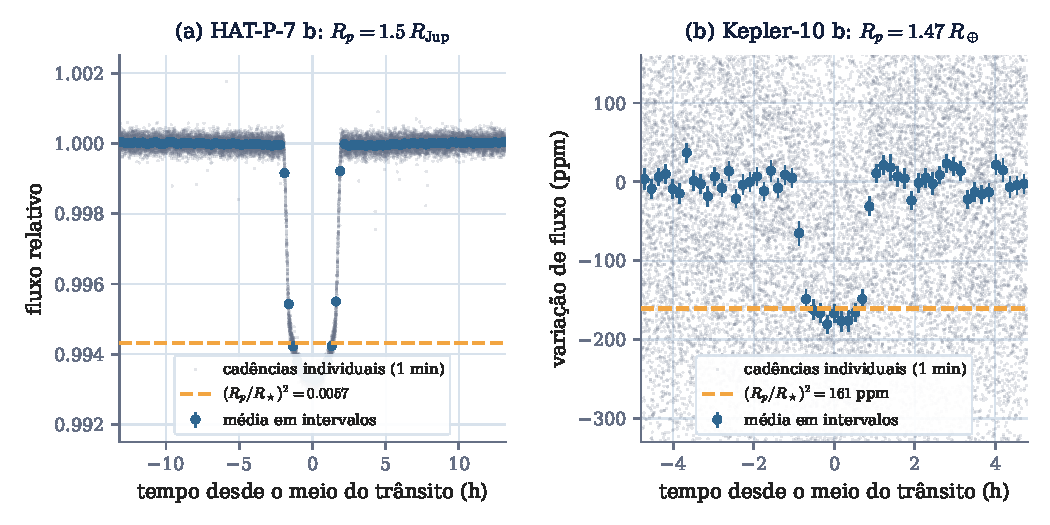
\includegraphics[width=\textwidth]{transito.pdf}
\caption{\textbf{Curvas de luz de trânsito reais, medidas pelo Kepler.} Fotometria de cadência curta (um ponto por minuto), dobrada no período orbital; os pontos cinza são cadências individuais e os círculos azuis são médias em intervalos de tempo. A linha tracejada não é ajuste algum: é a profundidade prevista por $(R_p/R_\star)^2$ com o raio do planeta e o raio da estrela medidos independentemente. \textbf{(a)} HAT-P-7\,b, um Júpiter quente diante de uma estrela de $2\,R_\odot$: a queda é de $0{,}57\%$ e o fundo achatado mostra o planeta inteiramente projetado sobre o disco estelar. \textbf{(b)} Kepler-10\,b, um planeta rochoso de $1{,}5\,R_\oplus$: a queda é de apenas $161$ partes por milhão, ou seja, $35$ vezes menor, exatamente como a razão dos raios ao quadrado prevê. É a mesma física nas duas escalas, e é por isso que a estatística de exoplanetas nasceu dominada por planetas grandes. Dados: arquivo público do Kepler (MAST); efemérides do NASA Exoplanet Archive.}
\end{figure}

Quando combinamos trânsito e velocidade radial, podemos obter raio e massa, logo densidade média. A densidade ajuda a distinguir mundos rochosos, ricos em água, gasosos ou com envelopes leves. Ainda assim, degenerescências permanecem: composições diferentes podem produzir massas e raios parecidos. Atmosferas exoplanetárias são investigadas por espectroscopia de trânsito, emissão secundária e curvas de fase, mas os sinais são pequenos. A interpretação exige modelos cuidadosos de nuvens, composição, temperatura, atividade estelar e ruído instrumental.

\textbf{Exemplo guiado.} Em um trânsito, a queda relativa de fluxo é aproximadamente $(R_p/R_\star)^2$. Um planeta do tamanho de Júpiter diante de uma estrela do tamanho do Sol tem $R_p/R_\star\simeq0{,}1$, produzindo queda de cerca de 1\%. Um planeta do tamanho da Terra tem $R_p/R_\star\simeq0{,}009$, produzindo queda de aproximadamente 0,008\%. A diferença mostra por que detectar Terras exige fotometria extremamente precisa.

\textbf{Perguntas para discussão.}
\begin{itemize}
\item Por que a linha de gelo influencia a formação de gigantes?
\item Que vieses observacionais moldam o catálogo conhecido de exoplanetas?
\item Por que densidade média não determina composição de forma única?
\item Como luas podem ser astrobiologicamente interessantes mesmo fora da zona habitável clássica?
\end{itemize}

\textbf{Para praticar.} Monte uma tabela com quatro mundos: Terra, Vênus, Europa e um exoplaneta fictício em zona habitável. Compare fonte de energia, atmosfera, água, estabilidade climática e métodos de detecção. A meta é perceber que habitabilidade é um problema multidimensional, não um selo simples aplicado por distância orbital.

\begin{lessonblock}[borderline west={2pt}{0pt}{astroGold}]{Dedução curta: temperatura de equilíbrio}
Um planeta a distância $a$ intercepta uma potência $\pi R_p^2 L_\star/(4\pi a^2)$. Se reflete uma fração $A$ dessa luz, absorve $(1-A)L_\star R_p^2/(4a^2)$. Emitindo como corpo negro por toda a superfície, perde $4\pi R_p^2\sigma T_{\rm eq}^4$. Igualando absorção e emissão:
\[
(1-A)\frac{L_\star}{4\pi a^2}\pi R_p^2=4\pi R_p^2\sigma T_{\rm eq}^4,
\]
\[
T_{\rm eq}=\left[\frac{(1-A)L_\star}{16\pi\sigma a^2}\right]^{1/4}.
\]
O raio do planeta cancela: no modelo mais simples, a temperatura de equilíbrio depende da estrela, da distância, do albedo e da redistribuição de calor. Atmosferas reais podem alterar drasticamente a superfície.
\end{lessonblock}

Exoplanetas ampliam o laboratório. Trânsitos medem raios relativos; velocidades radiais medem massas mínimas; juntos fornecem densidade média. Mas densidade não determina composição de forma única. Um planeta de baixa densidade pode ter envelope de hidrogênio; um planeta de densidade intermediária pode misturar rocha, água e gás; nuvens podem mascarar assinaturas atmosféricas. O catálogo de exoplanetas é também um catálogo de vieses observacionais.

\begin{figure}[htbp]
\centering
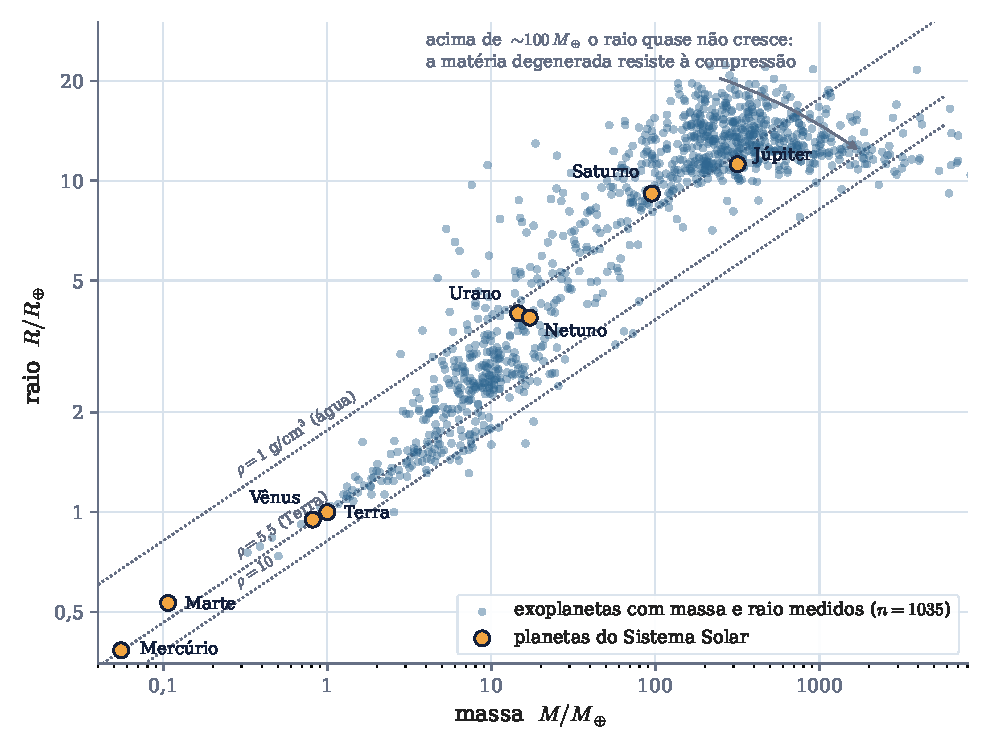
\includegraphics[width=0.94\textwidth]{massa_raio.pdf}
\caption{\textbf{Diagrama massa-raio: o que a densidade média entrega e o que ela esconde.} Todos os exoplanetas com massa verdadeira (não $M\sin i$) e raio medidos com precisão melhor que $25\%$ e $10\%$, respectivamente, junto com os planetas do Sistema Solar. As linhas pontilhadas são apenas geometria, $R=(3M/4\pi\rho)^{1/3}$, sem nenhum modelo de interior. Duas leituras importam. Primeira: massa e raio dão a densidade média, e a densidade já separa mundos rochosos (próximos da linha de $5{,}5$ g/cm$^3$, a da Terra) de mundos com envelope volumoso. Segunda: a dispersão vertical em cada massa mostra que a densidade \emph{não} determina composição --- planetas de mesma massa ocupam raios muito diferentes conforme tenham ou não envelope de hidrogênio, e acima de $\sim\!100\,M_\oplus$ o raio praticamente satura, porque a matéria degenerada resiste à compressão. Dados: NASA Exoplanet Archive, tabela \texttt{pscomppars}, consultada em julho de 2026.}
\end{figure}

\observaveis{profundidade de trânsito, período, velocidade radial, espectro de trânsito}{raio, distância orbital, massa mínima, composição atmosférica}{raio estelar, inclinação, atividade estelar, modelo atmosférico}{O método seleciona quais planetas são fáceis de encontrar e quais ficam escondidos?}

\textbf{Exemplo resolvido.} Um trânsito com profundidade de $1\%$ implica $(R_p/R_\star)^2=0{,}01$, logo $R_p/R_\star=0{,}1$. Se a estrela tem raio solar, o planeta tem raio de ordem joviana. Para uma Terra diante de um Sol, a profundidade é cerca de $0{,}008\%$. A diferença explica por que a estatística de exoplanetas nasceu dominada por planetas grandes e próximos.

\begin{lessonblock}[borderline west={2pt}{0pt}{astroGold}]{Dedução curta: densidade média como primeiro diagnóstico}
Com massa e raio, a densidade média é
\[
\rho=\frac{M}{(4/3)\pi R^3}.
\]
Em forma relativa à Terra,
\[
\frac{\rho}{\rho_\oplus}=\frac{M/M_\oplus}{(R/R_\oplus)^3}.
\]
Um planeta com $M=8M_\oplus$ e $R=2R_\oplus$ tem $\rho\simeq\rho_\oplus$. Isso sugere composição rochosa ou rica em materiais densos, mas não resolve a estrutura interna. Já $M=8M_\oplus$ e $R=3R_\oplus$ daria $\rho\simeq0{,}30\rho_\oplus$, indicando envelope volátil ou gasoso relevante.
\end{lessonblock}

\begin{lessonblock}{Leitura física: espectroscopia de trânsito}
Durante um trânsito, parte da luz estelar atravessa a atmosfera do planeta. Moléculas e átomos absorvem em comprimentos de onda específicos, alterando ligeiramente a profundidade do trânsito com $\lambda$. A assinatura é pequena porque a atmosfera é uma borda fina comparada ao disco estelar. Por isso a pergunta correta não é apenas ``qual molécula aparece?'', mas também: qual é o raio estelar? há nuvens? a estrela tem manchas? o sinal se repete em outros trânsitos?
\end{lessonblock}
\subsection*{Espectroscopia de atmosferas na era do JWST}

Medir a atmosfera de um planeta a centenas de anos-luz parece impossível, e quase é: a assinatura tem tamanho de partes por milhão. A técnica principal é a \textbf{espectroscopia de transmissão}. Durante o trânsito, uma fina coroa da atmosfera do planeta é atravessada pela luz da estrela. Onde a atmosfera absorve, ela fica efetivamente mais opaca, o raio aparente do planeta cresce e o trânsito fica ligeiramente mais profundo. Medindo a profundidade do trânsito em função do comprimento de onda, obtém-se um espectro do terminador do planeta.

A escala do efeito é dada pela altura de escala atmosférica,
\[
H=\frac{kT}{\mu g},
\]
e o sinal esperado é da ordem de $2R_pH/R_\star^{2}$ em profundidade relativa. Para um Júpiter quente, isso dá algumas centenas de partes por milhão; para um planeta rochoso temperado em torno de uma estrela solar, poucas partes por milhão --- o que explica por que os primeiros resultados vieram de planetas grandes, quentes e inflados, e não de gêmeos da Terra.

O JWST mudou o patamar dessa medida. Entre os resultados iniciais está a primeira detecção inequívoca de dióxido de carbono na atmosfera de um exoplaneta, no Júpiter quente WASP-39\,b, com significância que não deixa margem a debate, além de medidas de água, dióxido de enxofre --- indicando fotoquímica induzida pela estrela --- e nuvens. Para planetas menores há resultados em atmosferas de sub-Netunos e limites cada vez mais restritivos para planetas rochosos do sistema TRAPPIST-1, alguns dos quais parecem não ter atmosfera espessa alguma.

\begin{lessonblock}[borderline west={2pt}{0pt}{astroGold}]{Dedução curta: o vale de raios}
Um levantamento com precisão suficiente revela que planetas pequenos não se distribuem uniformemente em raio: há um déficit em torno de $1{,}8\,R_\oplus$, separando ``super-Terras'' de ``sub-Netunos''. A explicação mais aceita é perda de atmosfera.

Um envelope de hidrogênio de poucos por cento em massa infla enormemente o raio. Se a radiação ultravioleta da estrela --- ou o calor interno remanescente da formação --- consegue evaporar esse envelope, o planeta encolhe rapidamente até o raio do núcleo rochoso, atravessando a região intermediária em pouco tempo. Poucos planetas são flagrados no meio da transição, e é isso que abre o vale.

O ponto pedagógico: uma característica estatística de um catálogo --- um buraco em um histograma --- carrega informação sobre um processo físico que nunca foi observado diretamente em nenhum planeta individual.
\end{lessonblock}

\subsection*{Vieses de seleção, explicitamente}

Todo catálogo de exoplanetas é um retrato do método que o produziu, e não da natureza. Trânsitos exigem alinhamento: a probabilidade geométrica de um planeta transitar é aproximadamente $R_\star/a$, ou seja, $0{,}5\%$ para um análogo da Terra e $10\%$ para um Júpiter quente. Velocidades radiais favorecem planetas massivos e próximos, porque a amplitude escala com $M_p\sin i/\sqrt{a}$. Imageamento direto favorece planetas jovens, quentes, gigantes e muito afastados. Microlente é sensível a planetas em separações intermediárias, mas os eventos não se repetem.

Isso significa que qualquer afirmação sobre ``quantos planetas existem'' exige corrigir por completude --- estimar quantos planetas de cada tipo seriam detectados se existissem, e dividir. As estatísticas de ocorrência resultantes, do Kepler e do TESS, indicam que planetas pequenos são comuns e que uma fração significativa de estrelas de baixa massa hospeda planetas em zona habitável. A frase ``planetas são comuns'' não é uma leitura direta do catálogo; é uma conclusão obtida depois de desfazer o viés.

\subsection*{Habitabilidade: o que a zona habitável não diz}

A zona habitável é definida como a faixa de distâncias em que água líquida poderia existir na superfície, dadas a luminosidade estelar e hipóteses simples sobre atmosfera e albedo. É um conceito útil como primeiro filtro, e enganoso se levado ao pé da letra. Ele não considera composição atmosférica, efeito estufa, campo magnético, atividade estelar, rotação síncrona em torno de anãs vermelhas, tectônica ou entrega de voláteis. Vênus e Marte estão ambos nas bordas da zona habitável solar e são inóspitos por razões que a definição não captura.

O caso das anãs M ilustra bem a tensão: elas são as estrelas mais numerosas, seus planetas são mais fáceis de detectar e caracterizar, e a zona habitável fica próxima --- mas justamente por isso os planetas sofrem travamento de maré e são bombardeados por explosões estelares intensas durante bilhões de anos. Se atmosferas sobrevivem a esse ambiente é uma pergunta observacional em aberto, e é exatamente o que os programas do JWST em TRAPPIST-1 estão tentando responder.

\textbf{Perguntas para discussão.}
\begin{itemize}
\item Por que a espectroscopia de transmissão mede o terminador, e não o lado diurno?
\item Um planeta rochoso e um sub-Netuno podem ter o mesmo raio? E a mesma densidade média?
\item Como corrigir um catálogo de trânsitos pela probabilidade geométrica de alinhamento?
\item Que evidência elevaria uma molécula do status de ``detecção'' ao de ``biossinatura''? (Volte a esta pergunta no Capítulo 18.)
\end{itemize}

\begin{lessonblock}[borderline west={2pt}{0pt}{astroGold}]{Laboratório de dados 8 -- medir o raio de um planeta em outra estrela}
\textbf{Arquivos:} \texttt{10b\_transito\_kepler.csv} (curvas de luz reais do Kepler, dobradas no período orbital, para HAT-P-7\,b e Kepler-10\,b) e \texttt{10a\_exoplanetas\_massa\_raio.csv} (1035 planetas com massa e raio medidos).

\textbf{Física.} A profundidade do trânsito é a razão de áreas, e massa com raio dão densidade:
\[
\delta=\frac{\Delta F}{F}=\left(\frac{R_p}{R_\star}\right)^{2},
\qquad
\rho=\frac{3M}{4\pi R^{3}}.
\]

\textbf{Roteiro.}
\begin{enumerate}
\item Filtre o arquivo pelo planeta HAT-P-7\,b. Calcule a média do fluxo fora do trânsito ($|t|>3\,\mathrm{h}$) e a média dentro ($|t|<1\,\mathrm{h}$). A diferença relativa é $\delta$.
\item Extraia $R_p/R_\star$ e, com $R_\star=2{,}00\,R_\odot$, obtenha $R_p$ em raios de Júpiter.
\item Repita para Kepler-10\,b, com $R_\star=1{,}065\,R_\odot$. Aqui a queda é de poucas centenas de partes por milhão --- você vai precisar de médias em intervalos para enxergá-la.
\item No segundo arquivo, calcule a densidade média de todos os planetas e faça o histograma. Marque a posição da Terra ($5{,}51\,\mathrm{g/cm^3}$) e de Júpiter ($1{,}33$).
\end{enumerate}

\textbf{Entrega.} Os dois raios planetários medidos por você, com a comparação aos valores de catálogo, e o histograma de densidades com um comentário sobre o que ele revela de composição.

\textbf{Confira.} Medindo direto no arquivo, HAT-P-7\,b dá $\delta\simeq0{,}0066$, ou seja $R_p/R_\star\simeq0{,}081$ e $R_p\simeq1{,}6\,R_{\rm Jup}$ --- cerca de $7\%$ acima do valor de catálogo ($0{,}0754$). A diferença não é erro de medida: é o \textbf{escurecimento de bordo}, que torna o centro do disco estelar mais brilhante que a borda, de modo que o planeta bloqueia mais luz do que a razão de áreas sozinha prevê. Extrair $R_p/R_\star$ com precisão exige ajustar um modelo com esse efeito. Kepler-10\,b dá $\delta\simeq1{,}7\times10^{-4}$ e $R_p\simeq1{,}5\,R_\oplus$, contra $1{,}47$ de catálogo.
\end{lessonblock}

\newpage
\section*{Capítulo 11 -- Via Láctea, dinâmica galáctica e matéria escura}
\addcontentsline{toc}{section}{Capítulo 11 -- Via Láctea, dinâmica galáctica e matéria escura}
Galáxias são sistemas gravitacionais compostos por estrelas, gás, poeira, remanescentes, matéria escura e buracos negros centrais. A Via Láctea contém disco, bojo, halo, braços espirais e populações estelares de idades e composições diferentes. O Sol está no disco, longe do centro, orbitando a Galáxia em centenas de milhões de anos. Nossa posição interna torna o estudo da Via Láctea ao mesmo tempo rico e difícil: temos medidas detalhadas de estrelas próximas, mas a poeira e a perspectiva interna complicam a visão global.

Curvas de rotação galácticas são uma das evidências clássicas de matéria escura. Se a maior parte da massa estivesse concentrada na região luminosa central, esperaríamos velocidades orbitais decrescentes em grandes raios. Em muitas galáxias, as velocidades permanecem aproximadamente constantes. Isso sugere a presença de halos massivos de matéria não luminosa. A interpretação moderna combina curvas de rotação, lentes gravitacionais, dinâmica de aglomerados, CMB e formação de estruturas. Matéria escura não é uma ideia isolada para resolver um único gráfico; ela aparece em várias escalas.

\begin{figure}[htbp]
\centering
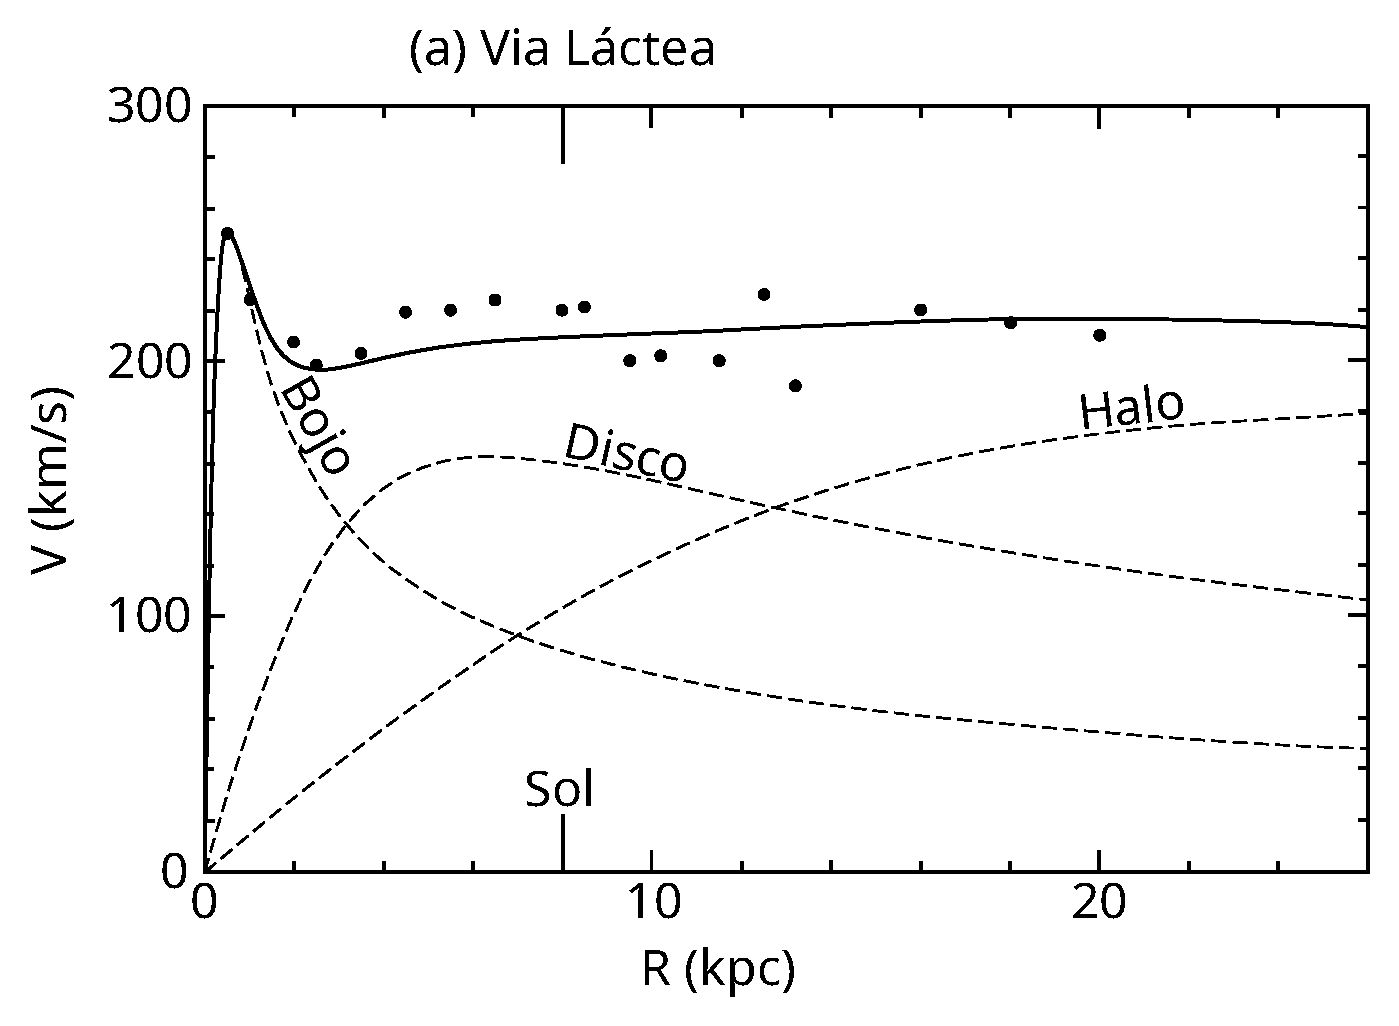
\includegraphics[width=0.49\textwidth]{rotacao_via_lactea.pdf}\hfill
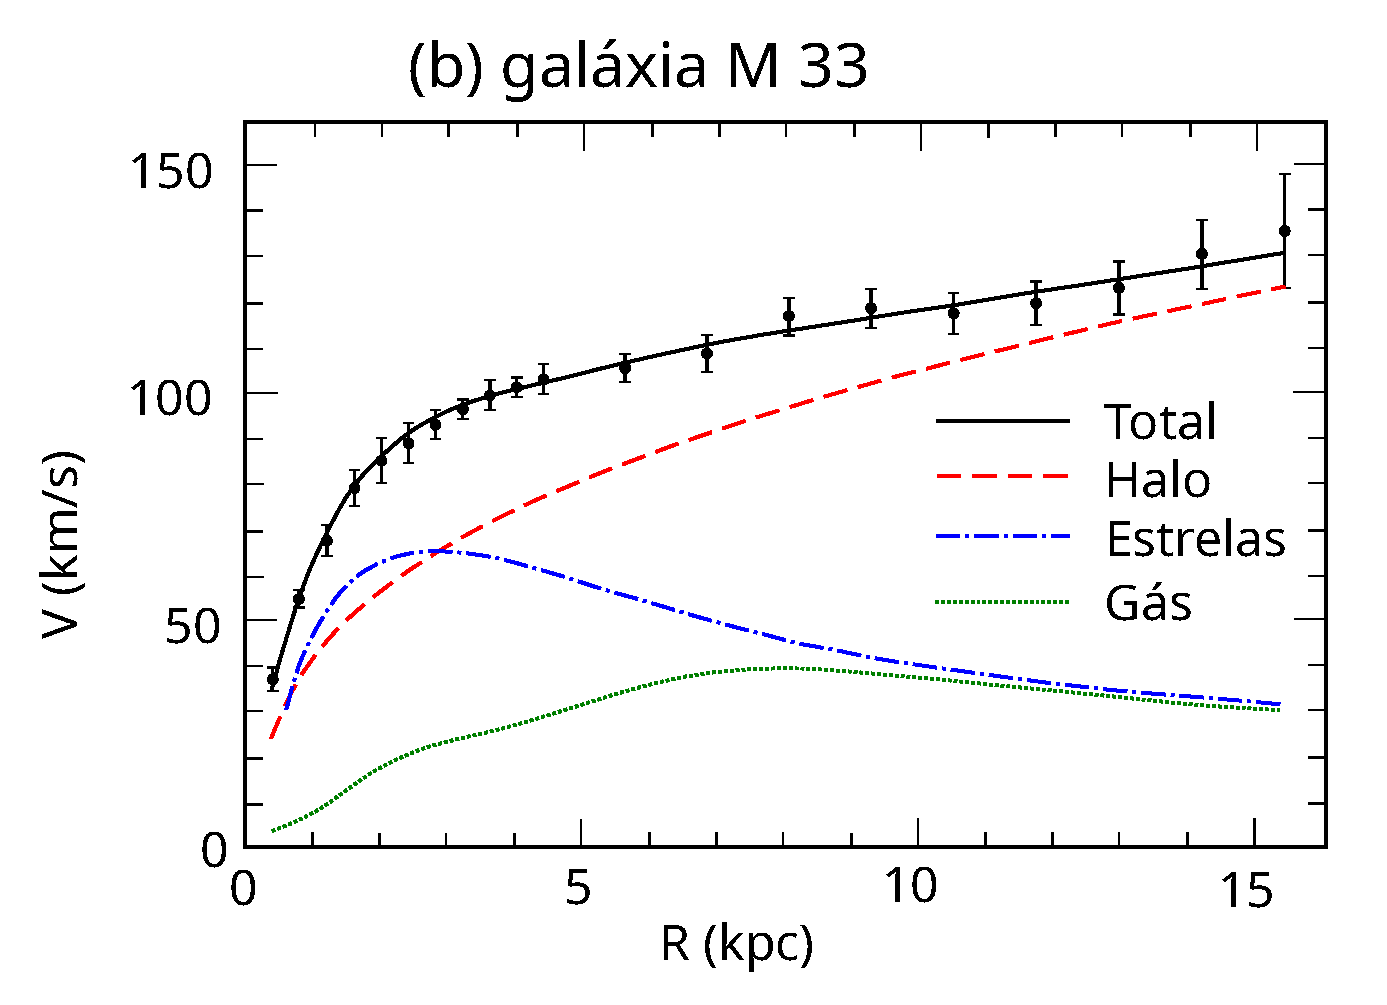
\includegraphics[width=0.49\textwidth]{rotacao_m33.pdf}
\caption{\textbf{Curvas de rotação e a massa que não se vê.} Os pontos são velocidades circulares medidas; as linhas tracejadas mostram quanto cada componente de massa contribuiria sozinha, e a linha cheia é a soma. \textbf{(a)} Na Via Láctea, bojo e disco explicam bem a curva perto do centro, mas caem rápido depois; para manter a velocidade praticamente constante até $R\simeq25\,\mathrm{kpc}$ é preciso uma componente adicional que \emph{cresce} com o raio --- o halo. O Sol está a cerca de $8\,\mathrm{kpc}$, ou seja, já na região onde o halo importa. \textbf{(b)} Em M 33 a decomposição é ainda mais clara: a contribuição das estrelas atinge um máximo em torno de $3\,\mathrm{kpc}$ e decresce, a do gás é pequena, e a curva observada continua subindo. O ponto não é que a curva seja ``plana'', e sim que ela não cai como cairia se a massa terminasse onde termina a luz. Figuras de Vallastro, via Wikimedia Commons, licença CC BY-SA 4.0; rótulos traduzidos para o português.}
\end{figure}
\subsection*{A anatomia da Galáxia}

A Via Láctea é uma espiral barrada com quatro componentes estruturais que têm cinemática, idade e composição distintas.

O \textbf{disco fino} concentra o gás, a poeira e a formação estelar atual; tem espessura de algumas centenas de parsecs, estrelas de todas as idades e metalicidade próxima da solar. O \textbf{disco espesso} é mais antigo, mais pobre em metais e cinematicamente mais quente --- suas estrelas oscilam mais para fora do plano. O \textbf{bojo}, com a barra central, é uma mistura complexa de populações velhas. E o \textbf{halo} estende-se por dezenas de kiloparsecs, contendo aglomerados globulares, estrelas muito pobres em metais e a maior parte da massa, na forma de matéria escura.

O Sol fica a cerca de $8\,\mathrm{kpc}$ do centro, dentro do disco, e completa uma volta em torno da Galáxia em aproximadamente $230$ milhões de anos. Essa posição interna é uma dificuldade metodológica séria: medimos a estrutura de dentro, com poeira bloqueando a visão do centro no óptico, e precisamos reconstruir a geometria tridimensional a partir de projeções e distâncias individuais.

\subsection*{O que o Gaia mudou}

Antes do Gaia, distâncias estelares confiáveis existiam para algumas dezenas de milhares de estrelas próximas. Depois dele, existem para mais de um bilhão, junto com movimentos próprios e, para milhões de estrelas, velocidades radiais. Isso converteu a Galáxia de um objeto essencialmente estático em um sistema dinâmico observável: passou a ser possível medir órbitas individuais, reconstruir o campo gravitacional e recuperar a história de acreção.

Três resultados dão a dimensão da mudança.

Primeiro, a descoberta de que boa parte do halo interno é formada por detritos de uma única fusão maior, ocorrida há cerca de dez bilhões de anos com uma galáxia anã hoje chamada Gaia-Enceladus. Suas estrelas são identificadas não por onde estão, mas por como se movem: elas ocupam uma região distinta no espaço de energia e momento angular.

Segundo, o mapeamento de \textbf{correntes estelares} --- aglomerados globulares e galáxias satélites sendo dilacerados por maré, deixando rastros finos de estrelas. A forma dessas correntes é sensível ao potencial gravitacional em que se movem, e lacunas nelas podem indicar encontros com concentrações escuras de massa. É hoje uma das sondas mais promissoras da subestrutura do halo de matéria escura.

Terceiro, a constatação de que o disco não está em equilíbrio: há ondulações verticais e padrões em espiral no espaço de fase, provavelmente resquícios da passagem recente da galáxia anã de Sagitário. A Via Láctea é um sistema com história recente, não um objeto relaxado.

\subsection*{O centro galáctico}

A região central concentra aglomerados estelares densos, gás molecular, campos magnéticos intensos e, no meio de tudo, Sagitário A*. A prova de sua natureza compacta veio do acompanhamento das órbitas de estrelas individuais ao longo de décadas com óptica adaptativa, discutido no Capítulo 7: a estrela S2 orbita com período de $\sim16$ anos e chega a $120$ unidades astronômicas do centro, o que confina $4\times10^{6}\,M_\odot$ dentro de uma região menor que o Sistema Solar. Nenhum aglomerado de objetos escuros conhecido sobreviveria estável nessa densidade, o que deixa buraco negro como única alternativa razoável.

A imagem do EHT em 2022 completou o quadro, mostrando o anel de emissão com o tamanho angular previsto. Vale registrar a diferença de dificuldade em relação a M\,87: Sagitário A* é muito menor, então o gás ao redor orbita em minutos, e a fonte muda enquanto está sendo observada. A imagem publicada é, por isso, uma média sobre estados variáveis --- detalhe metodológico que costuma passar despercebido.

\subsection*{A curva de rotação e o halo escuro}

A Figura~11 mostra o argumento central. Medindo velocidades de rotação em função do raio --- com gás neutro em $21\,\mathrm{cm}$, masers, gigantes e, hoje, com o próprio Gaia --- verifica-se que a velocidade circular permanece próxima de $220$--$240\,\mathrm{km\,s^{-1}}$ muito além da região onde há estrelas suficientes para explicá-la.

Vale ser preciso sobre o que isso implica. Em uma distribuição esférica, $v^{2}=GM(<r)/r$, então velocidade constante exige $M(<r)\propto r$: a massa continua crescendo linearmente com o raio, mesmo onde a luz já acabou. A densidade correspondente cai como $r^{-2}$. Não é que exista ``muita massa''; é que a massa está distribuída de um jeito completamente diferente da luz.

Essa conclusão vem acompanhada de várias outras, independentes: dispersão de velocidades em aglomerados de galáxias, lentes gravitacionais, o espectro de potência da radiação cósmica de fundo e a própria formação de estruturas. A força do argumento não está em nenhuma curva de rotação isolada, e sim na convergência de métodos que não compartilham hipóteses.

\begin{lessonblock}{Exemplo de aplicação: massa da Galáxia dentro da órbita solar}
Com $r_\odot=8{,}0\,\mathrm{kpc}=2{,}5\times10^{20}\,\mathrm{m}$ e $v=230\,\mathrm{km\,s^{-1}}$,
\[
M(<r_\odot)=\frac{rv^{2}}{G}=\frac{2{,}5\times10^{20}\times(2{,}3\times10^{5})^{2}}{6{,}67\times10^{-11}}\simeq2\times10^{41}\,\mathrm{kg}\simeq1\times10^{11}\,M_\odot.
\]
Contando estrelas, gás e poeira, chega-se a algo da ordem de $6\times10^{10}\,M_\odot$ nessa região --- já falta massa, embora pouco. O déficit cresce dramaticamente ao ir para fora: estimativas da massa total do halo, usando satélites e correntes estelares, ficam em torno de $10^{12}\,M_\odot$, dominadas por matéria escura. A discrepância não aparece de repente, ela se acumula com o raio.
\end{lessonblock}

\textbf{Perguntas para discussão.}
\begin{itemize}
\item Por que é mais difícil mapear a Via Láctea do que uma galáxia espiral externa?
\item O que exatamente uma curva de rotação plana implica sobre $M(<r)$ e sobre $\rho(r)$?
\item Como se identifica uma estrela ``de fora'' da Galáxia sem conhecer sua origem?
\item Que hipóteses entram ao converter a órbita de S2 em massa de Sagitário A*?
\item Por que correntes estelares são sondas úteis da subestrutura escura?
\end{itemize}

\textbf{Para praticar.} O arquivo público do Gaia permite consultas diretas. Selecione estrelas em um raio de $100\,\mathrm{pc}$ do Sol com paralaxe bem medida, construa o diagrama cor-magnitude absoluto e identifique a sequência principal, a sequência de anãs brancas e o ramo das gigantes. Depois compare com a Figura~4 e explique por que o diagrama de uma amostra limitada por volume tem aparência diferente do diagrama de uma amostra limitada por brilho.

\begin{lessonblock}[borderline west={2pt}{0pt}{astroGold}]{Laboratório de dados 9 -- pesar uma galáxia e encontrar o que falta}
\textbf{Arquivo:} \texttt{11\_curvas\_rotacao\_sparc.csv} --- curvas de rotação medidas de 176 galáxias, com a velocidade observada e as contribuições calculadas do gás, do disco estelar e do bojo.

\textbf{Física.} Para órbitas circulares, e somando componentes em quadratura:
\[
M(<r)=\frac{v^{2}r}{G},
\qquad
V_{\rm bárions}=\sqrt{V_{\rm gás}^{2}+V_{\rm disco}^{2}+V_{\rm bojo}^{2}}.
\]

\textbf{Roteiro.}
\begin{enumerate}
\item Escolha uma galáxia com muitos pontos (por exemplo NGC\,3198 ou NGC\,2403). Filtre as linhas correspondentes.
\item Faça o gráfico de $V_{\rm obs}$ contra o raio, com barras de erro, e sobreponha $V_{\rm bárions}$.
\item Calcule $M(<r)$ a partir de $V_{\rm obs}$ e, separadamente, a partir de $V_{\rm bárions}$. Use $r$ em metros ($1\,\mathrm{kpc}=3{,}086\times10^{19}\,\mathrm{m}$) e $v$ em m/s; divida por $M_\odot=1{,}989\times10^{30}\,\mathrm{kg}$.
\item Monte a razão $M_{\rm total}/M_{\rm bárions}$ em função do raio. Ela cresce, cai ou fica constante?
\item Repita para uma galáxia anã e para uma espiral massiva. A discrepância é igual nas duas?
\end{enumerate}

\textbf{Entrega.} As duas curvas sobrepostas, o gráfico da razão de massas contra o raio e uma resposta: em que raio a matéria não luminosa passa a dominar?

\textbf{Confira.} Para NGC\,3198, $V_{\rm obs}$ fica próximo de $150\,\mathrm{km\,s^{-1}}$ até $30\,\mathrm{kpc}$, enquanto a previsão bariônica cai. Em $r=30\,\mathrm{kpc}$, $M(<r)\simeq1{,}6\times10^{11}\,M_\odot$.
\end{lessonblock}

\newpage
\section*{Capítulo 12 -- Galáxias, interações e núcleos ativos}
\addcontentsline{toc}{section}{Capítulo 12 -- Galáxias, interações e núcleos ativos}
Galáxias são classificadas morfologicamente como espirais, elípticas, lenticulares e irregulares, mas essa classificação é apenas uma entrada para a física. Espirais têm discos, gás frio e formação estelar ativa. Elípticas costumam ter populações mais velhas e menos gás frio, embora haja exceções. Interações e fusões transformam morfologias, disparam surtos de formação estelar, alimentam núcleos ativos e redistribuem momento angular. A aparência de uma galáxia é resultado de massa, ambiente, história de acreção, gás disponível e feedback.

\imagemastro{0.72}{m51_hubble.jpg}{Galáxia espiral M51}{A estrutura espiral e a interação com a companheira tornam M51 um bom exemplo visual de morfologia, formação estelar e efeitos gravitacionais. Crédito: NASA, ESA, Hubble Heritage Team e colaboradores, via Wikimedia Commons.}

Formação estelar em galáxias depende de gás frio e denso. Braços espirais não são necessariamente conjuntos fixos de estrelas, mas padrões dinâmicos por onde gás pode ser comprimido. Regiões HII, nebulosas moleculares e estrelas jovens traçam locais recentes de formação. Já populações antigas informam a história acumulada. A metalicidade, isto é, a abundância de elementos mais pesados que hélio, funciona como registro químico: gerações anteriores de estrelas enriquecem o meio interestelar, alterando a composição das gerações seguintes.

A escada de distâncias extragalácticas combina métodos calibrados em sequência. Paralaxe calibra estrelas próximas; Cefeidas calibram distâncias em galáxias próximas; supernovas Ia alcançam distâncias maiores; redshift entra em escalas cosmológicas. Cada degrau carrega incertezas próprias. A robustez vem da sobreposição: métodos diferentes precisam concordar onde seus domínios se cruzam. A lei de Hubble-Lemaître, $v=H_0d$, emerge ao observar que galáxias distantes apresentam redshift proporcional à distância, interpretado como expansão cósmica.

Em grandes escalas, galáxias não se distribuem aleatoriamente. Elas formam grupos, aglomerados, filamentos, paredes e vazios. Essa teia cósmica resulta do crescimento gravitacional de pequenas flutuações iniciais. Simulações cosmológicas mostram como matéria escura estrutura potenciais gravitacionais nos quais gás cai, esfria e forma galáxias. Feedback de supernovas e núcleos ativos regula o processo, impedindo que toda matéria bariônica vire estrela de maneira simples. A formação de galáxias é um problema de múltiplas escalas: do parsec de regiões de formação estelar ao megaparsec de ambientes cósmicos.

Núcleos ativos de galáxias mostram que buracos negros supermassivos podem liberar enorme energia por acreção. O material que cai forma discos quentes, jatos relativísticos e regiões emissoras compactas. Quasares são AGNs muito luminosos, visíveis a grandes distâncias, e funcionam como sondas do universo jovem e do meio intergaláctico. O modelo unificado de AGN usa orientação, obscurecimento, disco, toro e jatos para explicar classes observacionais diferentes. Ainda assim, evolução temporal, ambiente e taxa de acreção também importam.

\textbf{Exemplo guiado.} Se uma galáxia tem velocidade de rotação aproximadamente constante $v$ em raio $r$, a massa interna inferida por órbita circular é $M(<r)\simeq v^2r/G$. Se $v$ não diminui quando $r$ cresce, a massa interna continua aumentando com o raio. Essa é a essência da evidência dinâmica para halos extensos: a luz pode cair, mas a massa gravitacional inferida continua relevante.

\textbf{Perguntas para discussão.}
\begin{itemize}
\item Por que a Via Láctea é difícil de mapear apesar de estarmos dentro dela?
\item Como curvas de rotação apontam para massa não luminosa?
\item Por que morfologia galáctica não é uma classificação puramente visual?
\item Que papel o ambiente desempenha na evolução de galáxias?
\end{itemize}

\textbf{Para praticar.} Use uma curva de rotação simplificada com valores de $v$ em diferentes raios. Calcule massas internas proporcionais a $v^2r$ e compare com um perfil luminoso hipotético. A conclusão importante é que a massa dinâmica pode crescer além da região onde a luz domina. A partir daí, registre hipóteses, incertezas e evidências independentes de matéria escura.

\begin{lessonblock}[borderline west={2pt}{0pt}{astroGold}]{Dedução curta: curva de rotação e massa interna}
Para uma órbita circular em um potencial aproximadamente esférico, a aceleração centrípeta é $v^2/r$ e a aceleração gravitacional é $GM(<r)/r^2$. Igualando:
\[
\frac{v^2}{r}=\frac{GM(<r)}{r^2}
\quad\Rightarrow\quad
M(<r)=\frac{v^2r}{G}.
\]
Se a velocidade permanece quase constante em grandes raios, então $M(<r)\propto r$. Ou seja, a massa dinâmica continua crescendo onde a luz visível já pode ter caído bastante. Essa é a leitura essencial da curva plana.
\end{lessonblock}

\begin{lessonblock}{Exemplo de aplicação: massa dinâmica de uma galáxia}
Para $v=200\,\mathrm{km\,s^{-1}}$ em $r=10\,\mathrm{kpc}$,
\[
M(<r)\simeq\frac{(2\times10^5\,\mathrm{m\,s^{-1}})^2(3{,}1\times10^{20}\,\mathrm{m})}{6{,}67\times10^{-11}}
\simeq1{,}9\times10^{41}\,\mathrm{kg},
\]
ou cerca de $10^{11}M_\odot$. Se em $20\,\mathrm{kpc}$ a velocidade ainda for parecida, a massa interna dobra aproximadamente. Essa conta simples já mostra por que a dinâmica exige mais massa do que a luz sugere.
\end{lessonblock}

\subsection*{O universo jovem visto pelo JWST}

Observar galáxias distantes é observar o passado, e a barreira sempre foi o desvio para o vermelho: em $z=10$, a luz ultravioleta de estrelas jovens chega em $1$--$3\,\mu\mathrm{m}$, onde o Hubble mal alcança e a atmosfera terrestre atrapalha. Foi para isso que o JWST foi construído, e o resultado veio rápido.

Hoje há galáxias confirmadas espectroscopicamente em $z>13$, quando o universo tinha menos de $300$ milhões de anos --- uma fração de $2\%$ da idade atual. A confirmação espectroscópica importa: candidatos selecionados apenas por cor podem ser impostores, tipicamente galáxias poeirentas em desvio para o vermelho moderado, cuja distribuição de energia imita a de uma galáxia primordial. Vários candidatos anunciados nos primeiros meses caíram justamente nesse teste.

O que se aprendeu tem duas partes. Primeiro, galáxias se formam mais cedo e brilham mais do que a maioria dos modelos previa, o que exige formação estelar mais eficiente, menos poeira ou função de massa inicial diferente nas primeiras épocas. Segundo, apareceu uma população nova, os \textit{little red dots} --- objetos compactos e vermelhos, abundantes em $z\sim5$--$8$, cuja natureza (estrelas muito densas, núcleos ativos envoltos em gás, ou uma mistura) ainda está sendo debatida. Descobrir uma classe de objetos que não estava em nenhuma previsão é o tipo de resultado que justifica construir telescópios novos.

\subsection*{Buracos negros e galáxias crescem juntos}

Praticamente toda galáxia massiva tem um buraco negro supermassivo no centro, e a massa desse buraco negro correlaciona-se fortemente com propriedades da galáxia hospedeira --- em particular com a dispersão de velocidades do bojo, na chamada relação $M_{\rm BH}$--$\sigma$. A correlação é notável porque as escalas são absurdamente diferentes: a esfera de influência gravitacional do buraco negro é milhares de vezes menor que a galáxia. Não há razão \emph{a priori} para que o centro saiba o que o resto está fazendo.

A explicação padrão é \textbf{feedback}: quando o buraco negro acreta, libera energia suficiente para aquecer e expelir gás da região central, cortando o próprio suprimento e também a formação estelar da galáxia. O sistema se auto-regula, e a relação observada seria a assinatura desse equilíbrio. Modelos de formação de galáxias praticamente não conseguem reproduzir a população observada sem incluir algum mecanismo desse tipo --- sem feedback, as simulações produzem galáxias grandes demais e com formação estelar em excesso.

\subsection*{Núcleos ativos: uma família, vários ângulos}

Quasares, blazares, galáxias Seyfert e rádio-galáxias foram catalogados como classes separadas antes de se entender que grande parte da diversidade é geométrica. No modelo unificado, todos têm o mesmo motor central --- disco de acreção em torno de um buraco negro supermassivo --- e as diferenças vêm da orientação em relação a nós, da presença ou não de um toro de poeira obscurecendo a região central e da existência de jatos relativísticos.

Se olhamos de frente para um jato, o efeito de \textit{beaming} relativístico amplifica enormemente o brilho e comprime as escalas de tempo observadas: é um blazar, com variabilidade de horas e emissão até em raios gama de altíssima energia. Se o toro fica na linha de visada, vemos linhas estreitas apenas, porque a região de linhas largas está escondida. Testar esse modelo exige, entre outras coisas, espectropolarimetria --- luz espalhada por elétrons acima do toro revela a região oculta por reflexão.

\subsection*{Lentes gravitacionais como instrumento}

Massa curva o espaço e desvia luz. Quando um aglomerado de galáxias fica alinhado com uma fonte distante, o resultado são arcos e imagens múltiplas, e o aglomerado funciona como uma lente natural que amplifica objetos de outro modo inacessíveis. Boa parte das galáxias mais distantes conhecidas foi encontrada atrás de aglomerados, com ampliações de fatores de dez ou mais.

A técnica tem duas leituras. Do lado da fonte, é um telescópio gratuito. Do lado da lente, a distorção mede a distribuição de massa total do aglomerado, incluindo a escura, sem qualquer hipótese sobre equilíbrio dinâmico --- o que a torna uma das evidências mais limpas de matéria escura. Em regime fraco, a distorção estatística das formas de milhões de galáxias de fundo mapeia a distribuição de massa em grande escala, e é justamente esse o método principal dos levantamentos Euclid e Rubin.

\begin{lessonblock}{Exemplo de aplicação: por que quasares são compactos}
Um quasar pode variar significativamente em brilho em uma escala de dias. Pela régua causal, a região emissora tem tamanho máximo
\[
R\lesssim c\,\Delta t=3\times10^{8}\times86400\simeq2{,}6\times10^{13}\,\mathrm{m},
\]
cerca de $170$ unidades astronômicas. Ou seja, uma fonte mais luminosa que uma galáxia inteira cabe dentro de algo comparável ao Sistema Solar. Nenhuma população de estrelas produz isso; acreção sobre um objeto compacto, sim. Esse argumento --- feito nos anos 1960, muito antes de qualquer imagem --- é o que estabeleceu buracos negros supermassivos como explicação necessária.
\end{lessonblock}

\textbf{Perguntas para discussão.}
\begin{itemize}
\item Por que a confirmação espectroscópica é indispensável para uma galáxia candidata em $z>10$?
\item Como uma correlação entre escalas tão distintas ($M_{\rm BH}$ e $\sigma$) pode ser fisicamente causada?
\item Que observações distinguiriam um blazar de uma Seyfert se ambos tivessem o mesmo motor central?
\item Lente forte e lente fraca medem coisas diferentes. Quais, e com que hipóteses?
\end{itemize}

\newpage
\section*{Capítulo 13 -- Cosmologia observacional e expansão do universo}
\addcontentsline{toc}{section}{Capítulo 13 -- Cosmologia observacional e expansão do universo}
Cosmologia estuda o universo em grandes escalas, onde a distribuição média de matéria e energia pode ser tratada de forma homogênea e isotrópica em primeira aproximação. Essa hipótese não diz que o universo é uniforme em escalas pequenas: estrelas, galáxias e aglomerados existem. Ela afirma que, em escalas suficientemente grandes, não há centro ou direção privilegiada evidente. O modelo cosmológico moderno combina relatividade geral, expansão observada, radiação cósmica de fundo, abundâncias primordiais e formação de estruturas.

A expansão cósmica é descrita pelo fator de escala. Galáxias distantes não se afastam simplesmente como projéteis atravessando espaço estático; em cosmologia relativística, o próprio espaço entre observadores comóveis se expande. O redshift cosmológico mede quanto o comprimento de onda da luz foi esticado desde a emissão. Para pequenos redshifts, a lei de Hubble-Lemaître aproxima a relação entre velocidade recessional e distância. Para grandes redshifts, é necessário usar o modelo cosmológico completo, com parâmetros de matéria, radiação, curvatura e energia escura.

A densidade crítica define a escala em que a geometria espacial é plana em modelos simples. Costumamos expressar componentes do universo por parâmetros $\Omega$: matéria bariônica, matéria escura, radiação e energia escura. Observações indicam que a matéria bariônica é apenas uma fração pequena do conteúdo total. Matéria escura domina a matéria gravitante em muitas escalas. Energia escura está associada à expansão acelerada observada no universo recente. Esses nomes resumem fenômenos medidos, mas não encerram as perguntas fundamentais sobre a natureza microscópica desses componentes.

A radiação cósmica de fundo é uma das evidências mais fortes do universo quente e denso. Ela possui espectro quase perfeito de corpo negro, com temperatura atual próxima de 2,7 K. Essa radiação foi liberada quando elétrons e prótons se combinaram em átomos neutros, tornando o universo transparente à luz. Antes disso, fótons eram espalhados frequentemente por elétrons livres. As pequenas anisotropias da CMB registram flutuações de densidade que mais tarde cresceriam para formar estruturas. Assim, um mapa de micro-ondas carrega informação sobre física do universo jovem.

\begin{figure}[htbp]
\centering
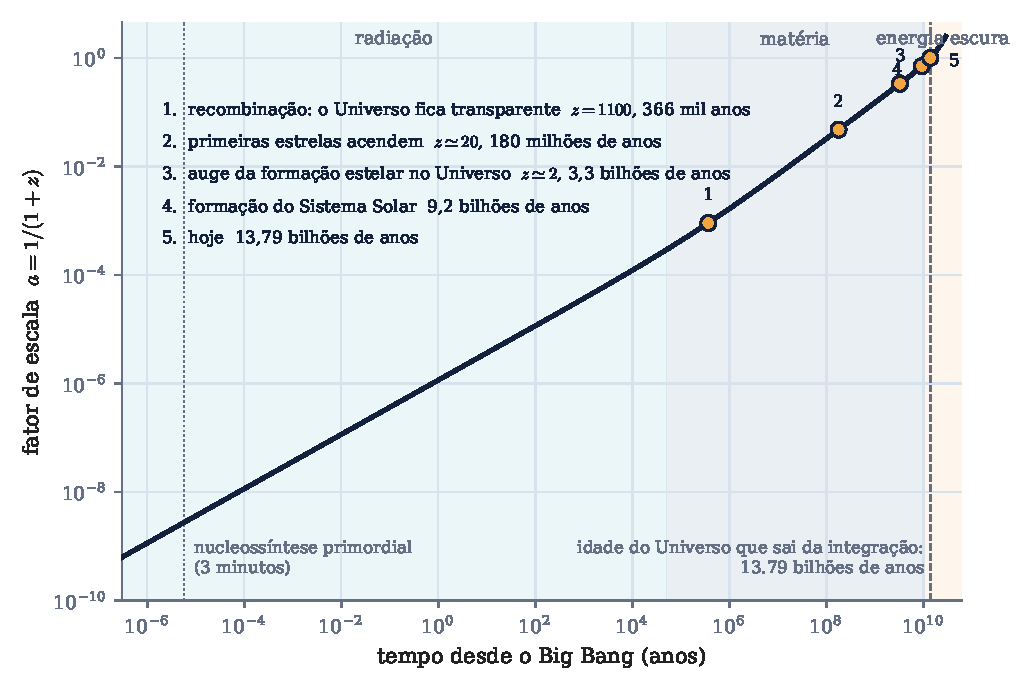
\includegraphics[width=\textwidth]{cosmologia.pdf}
\caption{\textbf{A linha do tempo cósmica, em escala logarítmica.} Fator de escala $a=1/(1+z)$ em função do tempo, obtido integrando a equação de Friedmann $H(a)=H_0\sqrt{\Omega_r a^{-4}+\Omega_m a^{-3}+\Omega_\Lambda}$ com os parâmetros do Planck 2018 ($H_0=67{,}4$ km/s/Mpc, $\Omega_m=0{,}315$). O eixo do tempo cobre dezessete ordens de grandeza porque não há alternativa: a nucleossíntese primordial dura minutos e a formação do Sistema Solar leva bilhões de anos. As faixas ao fundo marcam qual componente domina a densidade de energia --- radiação até $50$ mil anos, matéria até $10$ bilhões de anos, energia escura depois disso --- e a inclinação da curva muda em cada transição, de $a\propto t^{1/2}$ para $a\propto t^{2/3}$ e finalmente para crescimento exponencial. A posição de cada evento numerado não foi escolhida: entra o desvio para o vermelho e o tempo sai da integração. A idade do Universo também é resultado, não hipótese: $13{,}79$ bilhões de anos, contra os $13{,}80$ do Planck. Note ainda o que \emph{não} cabe na figura: a inflação acontece por volta de $10^{-36}$ s, cerca de trinta e sete ordens de grandeza à esquerda da borda do gráfico.}
\end{figure}

\imagemastro{0.84}{hudf_2014.jpg}{Campo ultraprofundo do Hubble}{Uma pequena região do céu contém milhares de galáxias em diferentes distâncias e épocas cósmicas, tornando a imagem uma janela para evolução galáctica. Crédito: NASA, ESA e Hubble, via ESA/Hubble.}
\subsection*{A escada de distâncias, degrau por degrau}

Nenhum método mede distâncias em todas as escalas. O que existe é uma sequência de técnicas, cada uma calibrada pela anterior --- e como em qualquer escada, um degrau torto desloca todos os de cima.

\begin{lessonblock}{A escada cósmica}
\begin{tabular}{>{\raggedright\arraybackslash}p{0.26\textwidth}>{\raggedright\arraybackslash}p{0.20\textwidth}>{\raggedright\arraybackslash}p{0.42\textwidth}}
\toprule
Método & Alcance típico & Sobre o que se apoia \\
\midrule
Paralaxe trigonométrica & até $\sim$ alguns kpc & Geometria pura; nenhuma hipótese astrofísica \\
Ajuste de sequência principal & $\sim$100 kpc & Modelos estelares e metalicidade \\
Cefeidas & até $\sim$40 Mpc & Relação período-luminosidade calibrada por paralaxes \\
Topo do ramo das gigantes & até $\sim$20 Mpc & Física do \textit{flash} do hélio \\
Supernovas Ia & até $\sim$1000 Mpc & Padronização da curva de luz, calibrada por Cefeidas ou TRGB \\
Lei de Hubble-Lemaître & além disso & Homogeneidade e valor de $H_0$ \\
\bottomrule
\end{tabular}
\end{lessonblock}

O Gaia refez o primeiro degrau com precisão sem precedentes, e isso propagou para cima: as calibrações de Cefeidas usadas hoje dependem diretamente de suas paralaxes. É um bom exemplo de como um avanço instrumental em uma escala reorganiza resultados em outra completamente diferente.

\subsection*{Supernovas Ia e a descoberta da aceleração}

Supernovas de tipo Ia não são idênticas, mas são \emph{padronizáveis}: existe uma relação empírica entre a largura da curva de luz e o brilho máximo --- as que declinam mais devagar são intrinsecamente mais luminosas. Corrigindo por essa relação, a dispersão cai para cerca de $0{,}15$ magnitude, o que as torna as melhores velas padrão em escala cosmológica.

No fim dos anos 1990, dois grupos independentes mediram supernovas distantes e encontraram-nas mais fracas do que um universo em desaceleração previa. A interpretação --- expansão acelerada, dominada por uma componente de pressão negativa --- rendeu o Nobel de 2011 e introduziu a energia escura no modelo padrão. Vale sublinhar o formato do argumento: não se ``viu'' energia escura. Mediram-se brilhos e desvios para o vermelho, comparou-se com previsões de modelos, e a única família de modelos compatível exigia aceleração.

\subsection*{Oscilações acústicas de bárions: uma régua, não uma vela}

Antes da recombinação, fótons e bárions formavam um fluido acoplado em que perturbações se propagavam como ondas sonoras. Quando o universo ficou transparente, essas ondas congelaram, deixando uma escala característica impressa tanto na radiação cósmica de fundo quanto na distribuição de galáxias: um excesso de pares de galáxias separadas por cerca de $150\,\mathrm{Mpc}$ comóveis.

Como essa escala é calculável a partir da física do plasma primordial, ela funciona como \textbf{régua padrão}. Medindo seu tamanho angular e sua extensão em desvio para o vermelho em diferentes épocas, obtém-se a história da expansão sem depender de velas padrão nem da escada de distâncias local. É uma via completamente independente, e é por isso que os levantamentos espectroscópicos de milhões de galáxias --- BOSS, eBOSS e hoje o DESI --- se tornaram centrais na cosmologia observacional.

\subsection*{Tensão de Hubble: o problema em aberto}

Medidas locais (Cefeidas mais supernovas Ia) dão $H_0\simeq73\,\mathrm{km\,s^{-1}\,Mpc^{-1}}$; a extrapolação a partir da radiação cósmica de fundo dá $\simeq67{,}4$. A discrepância é de cerca de cinco desvios-padrão e resistiu a uma década de escrutínio, incluindo verificações feitas com o JWST na fotometria das Cefeidas.

Este é, hoje, provavelmente o problema mais discutido da cosmologia, e ele é tratado em detalhe no Capítulo 18. Registre aqui apenas a estrutura lógica: um lado mede a expansão \emph{agora}, o outro mede parâmetros em $z\simeq1100$ e \emph{prevê} o valor de hoje usando o modelo. Se os dois discordam, ou uma das medidas tem erro sistemático, ou o modelo que faz a ponte entre elas está incompleto.

\begin{lessonblock}[borderline west={2pt}{0pt}{astroGold}]{Dedução curta: o que $z$ mede, afinal}
O desvio para o vermelho cosmológico não é efeito Doppler de galáxias movendo-se \emph{através} do espaço; é consequência da expansão do próprio espaço enquanto a luz viaja. A relação exata é
\[
1+z=\frac{a(t_{\rm obs})}{a(t_{\rm emis})}=\frac{1}{a(t_{\rm emis})},
\]
tomando $a=1$ hoje. Ou seja, $z$ mede diretamente \emph{quanto o universo se expandiu} desde a emissão, e não velocidade. Um objeto em $z=1$ emitiu sua luz quando todas as distâncias eram metade das atuais.

A conversão de $z$ em distância ou em tempo exige integrar a equação de Friedmann e, portanto, depende do modelo cosmológico --- foi exatamente esse o cálculo da Figura~13. Apenas para $z\ll1$ vale a aproximação linear $v\simeq cz$ e a lei $d\simeq cz/H_0$. Usar essa aproximação em $z=2$ é um erro comum e grosseiro.
\end{lessonblock}

\textbf{Perguntas para discussão.}
\begin{itemize}
\item Por que uma régua padrão é metodologicamente diferente de uma vela padrão?
\item Que degrau da escada de distâncias você suspeitaria primeiro diante da tensão de Hubble, e como testaria?
\item Se energia escura fosse dinâmica, que observável mudaria primeiro?
\item Por que $z$ não deve ser lido como velocidade em desvios para o vermelho altos?
\end{itemize}

\begin{lessonblock}[borderline west={2pt}{0pt}{astroGold}]{Laboratório de dados 10 -- medir a constante de Hubble}
\textbf{Arquivo:} \texttt{13\_supernovas\_ia\_pantheon.csv} --- 1573 supernovas de tipo Ia com desvio para o vermelho, módulo de distância e incerteza, da compilação Pantheon+.

\textbf{Física.} O módulo de distância converte-se em distância, e a lei de Hubble-Lemaître liga distância e velocidade:
\[
d\,[\mathrm{Mpc}]=10^{(\mu-25)/5},
\qquad
v\simeq cz,
\qquad
v=H_0d.
\]

\textbf{Roteiro.}
\begin{enumerate}
\item Calcule $d$ para todas as supernovas. No Excel: \texttt{=10\^{}((C2-25)/5)}.
\item Selecione apenas $z<0{,}1$, onde a aproximação $v\simeq cz$ vale, e faça o gráfico de $v$ contra $d$.
\item Ajuste uma reta passando pela origem. A inclinação é $H_0$, em $\mathrm{km\,s^{-1}\,Mpc^{-1}}$.
\item Calcule a idade aproximada do universo como $1/H_0$, convertendo unidades. Compare com os $13{,}8$ bilhões de anos da Figura~13.
\item Agora inclua todas as supernovas até $z=1{,}6$ e faça o gráfico de $\mu$ contra $\log z$. Estenda a reta ajustada em baixo $z$: os pontos de alto $z$ ficam acima ou abaixo dela? O que isso significa fisicamente?
\end{enumerate}

\textbf{Entrega.} O diagrama de Hubble, o valor de $H_0$ com incerteza, a idade estimada e um parágrafo interpretando o desvio em alto $z$.

\textbf{Confira.} Você deve obter algo entre $65$ e $70\,\mathrm{km\,s^{-1}\,Mpc^{-1}}$, dependendo do corte em $z$ e de usar ou não pesos --- e $1/H_0\simeq14$ bilhões de anos, próximo da idade real por coincidência numérica, não por identidade. O valor publicado pela colaboração é $73$: a diferença vem das correções de velocidade peculiar e do termo de desaceleração, que este roteiro simplificado ignora. Esse deslocamento é justamente o objeto do laboratório 11. Em alto $z$ as supernovas aparecem \emph{mais fracas} que o previsto sem energia escura: foi essa observação que rendeu o Nobel de 2011.
\end{lessonblock}

\newpage
\section*{Capítulo 14 -- Universo primordial e modelo cosmológico padrão}
\addcontentsline{toc}{section}{Capítulo 14 -- Universo primordial e modelo cosmológico padrão}
A nucleossíntese primordial ocorreu nos primeiros minutos, quando temperatura e densidade permitiram formar núcleos leves. O resultado principal foi hidrogênio, hélio e pequenas quantidades de deutério, hélio-3 e lítio. Elementos mais pesados exigem ambientes estelares e explosivos posteriores. A concordância entre abundâncias previstas e observadas é um teste importante do modelo. Ela também limita a quantidade de matéria bariônica: não podemos simplesmente declarar que toda matéria escura é gás comum frio sem violar essas evidências.

Inflação é uma hipótese para uma fase de expansão extremamente rápida no universo primordial. Ela foi proposta para explicar problemas como a homogeneidade do céu em regiões que, sem inflação, não teriam tido tempo causal para se equilibrar; a quase planura espacial; e a origem de flutuações iniciais. Em muitos modelos, flutuações quânticas esticadas pela inflação tornam-se sementes clássicas para a estrutura cósmica. A inflação não é uma única teoria fechada, mas uma família de cenários testados por previsões sobre anisotropias, polarização e distribuição de estruturas.

A expansão acelerada foi inferida de supernovas Ia distantes e hoje é sustentada por múltiplas observações combinadas. Energia escura pode ser representada, no modelo mais simples, por uma constante cosmológica. Mas a interpretação física permanece aberta: pode ser energia do vácuo, um campo dinâmico ou sinal de que a gravidade precisa ser entendida de outra forma em grandes escalas. A postura científica adequada é dupla: usar o modelo $\Lambda$CDM porque ele funciona muito bem, e ao mesmo tempo reconhecer que seus componentes escuros ainda pedem explicação profunda.

\textbf{Exemplo guiado.} Um redshift $z=1$ significa que o comprimento de onda observado é duas vezes o emitido, pois $1+z=\lambda_{\rm obs}/\lambda_{\rm em}$. Uma linha emitida em $400\,\mathrm{nm}$ seria observada em $800\,\mathrm{nm}$. Isso não deve ser interpretado como simples Doppler newtoniano em todos os casos; em cosmologia, o redshift acumula a expansão do universo ao longo da trajetória da luz.

\textbf{Perguntas para discussão.}
\begin{itemize}
\item Em que sentido o universo pode ser homogêneo se galáxias existem?
\item Por que a CMB é uma evidência tão forte de um universo quente no passado?
\item Como abundâncias de elementos leves limitam a quantidade de matéria bariônica?
\item O que significa aceitar um modelo cosmológico bem-sucedido sem conhecer totalmente a natureza de seus componentes?
\end{itemize}

\textbf{Para praticar.} Construa uma linha do tempo em escala logarítmica: inflação, nucleossíntese primordial, recombinação, primeiras estrelas, primeiras galáxias, formação do Sistema Solar e presente. Em cada marco, registre temperatura qualitativa, componentes dominantes e evidência observacional. A escala logarítmica é essencial: os primeiros segundos e os bilhões de anos posteriores precisam caber na mesma narrativa.

\begin{lessonblock}[borderline west={2pt}{0pt}{astroGold}]{Dedução curta: redshift e fator de escala}
Em cosmologia homogênea, comprimentos de onda acompanham a expansão do universo. Se $a(t)$ é o fator de escala, então
\[
1+z=\frac{\lambda_{\rm obs}}{\lambda_{\rm em}}=\frac{a(t_{\rm obs})}{a(t_{\rm em})}.
\]
Tomando $a(t_{\rm obs})=1$, um objeto em $z=3$ emitiu a luz quando o fator de escala era $a=1/4$. Isso não significa que ele estava simplesmente se movendo a uma velocidade newtoniana específica; significa que a luz foi esticada pela expansão acumulada entre emissão e observação.
\end{lessonblock}

\begin{lessonblock}{Exemplo de aplicação: densidade crítica}
A densidade crítica é
\[
\rho_c=\frac{3H_0^2}{8\pi G}.
\]
Usando $H_0\simeq70\,\mathrm{km\,s^{-1}\,Mpc^{-1}}\simeq2{,}3\times10^{-18}\,\mathrm{s^{-1}}$, obtemos
\[
\rho_c\simeq9\times10^{-27}\,\mathrm{kg\,m^{-3}}.
\]
O número parece absurdamente pequeno, mas em volumes cosmológicos ele controla a geometria e a história de expansão. Essa é uma boa lição de escala: densidade média cósmica não se compara intuitivamente com densidades de laboratório.
\end{lessonblock}

\subsection*{Três problemas que a inflação resolve}

O modelo do Big Bang quente descreve muito bem a evolução do universo a partir de frações de segundo, mas deixa três desconfortos que não são contradições e sim exigências de ajuste fino implausível.

\textbf{O problema do horizonte.} Regiões opostas do céu, vistas na radiação cósmica de fundo, têm a mesma temperatura com precisão de partes em cem mil. Só que, no modelo sem inflação, essas regiões nunca estiveram em contato causal: a luz não teve tempo de percorrer a distância entre elas desde o Big Bang. Por que teriam a mesma temperatura?

\textbf{O problema da planura.} A densidade do universo é hoje muito próxima do valor crítico. Como o desvio em relação ao valor crítico cresce com o tempo em um universo dominado por matéria ou radiação, estar próximo hoje exige ter estado absurdamente próximo no início --- ajuste de dezenas de casas decimais.

\textbf{Ausência de relíquias exóticas.} Teorias de grande unificação preveem produção abundante de monopolos magnéticos, que não são observados.

Uma fase de expansão acelerada exponencial nos primeiros instantes resolve os três de uma vez: ela põe em contato causal regiões que depois se separam, achata a geometria por esticamento, e dilui qualquer relíquia produzida antes. O preço é postular um campo escalar com propriedades adequadas, cuja identidade física permanece desconhecida.

O que torna a inflação interessante não é resolver problemas antigos --- teorias construídas para isso são baratas ---, e sim ter feito uma previsão nova e testável: as flutuações quânticas do campo, esticadas a escalas cosmológicas, produziriam um espectro de perturbações de densidade quase invariante de escala, ligeiramente inclinado, adiabático e gaussiano. As medidas da radiação cósmica de fundo confirmaram exatamente esse padrão, incluindo a leve inclinação. É uma das previsões bem-sucedidas mais impressionantes da física, e ainda assim insuficiente para identificar o mecanismo.

\subsection*{Nucleossíntese primordial: um teste com um parâmetro}

Entre cerca de um e vinte minutos após o Big Bang, o universo esteve na faixa de temperatura em que reações nucleares funcionam e núcleos leves sobrevivem. O resultado foi a produção de deutério, hélio-3, hélio-4 e traços de lítio-7. Elementos mais pesados não se formaram porque não há núcleos estáveis de massa 5 e 8, e a densidade caiu rápido demais.

O que torna esse cálculo poderoso é que ele tem essencialmente \emph{um} parâmetro livre: a razão entre bárions e fótons. Fixado esse número, as abundâncias de todos os núcleos leves ficam determinadas. E o valor extraído das abundâncias observadas concorda com o valor obtido de maneira totalmente independente pelo espectro de potência da radiação cósmica de fundo. Duas físicas diferentes, separadas por trezentos mil anos de história cósmica, apontando o mesmo número.

A exceção é o lítio-7, observado em estrelas velhas com abundância cerca de três vezes menor que a prevista --- o problema do lítio primordial, ainda em aberto (Capítulo 18).

\subsection*{A radiação cósmica de fundo, camada por camada}

\begin{lessonblock}{O que se lê na CMB}
\begin{tabular}{>{\raggedright\arraybackslash}p{0.30\textwidth}>{\raggedright\arraybackslash}p{0.60\textwidth}}
\toprule
Característica observada & O que ela mede \\
\midrule
Espectro de corpo negro perfeito a $2{,}725\,\mathrm{K}$ & Equilíbrio térmico no universo primitivo; nenhuma injeção significativa de energia posterior \\
Dipolo de $\sim3{,}4\,\mathrm{mK}$ & Movimento próprio do Sistema Solar em relação ao referencial da CMB \\
Posição do primeiro pico acústico & Geometria espacial: o universo é plano com boa precisão \\
Razão entre picos ímpares e pares & Densidade de bárions \\
Amortecimento nos picos altos & Espessura da superfície de último espalhamento \\
Polarização em modo E & Consistência do quadro de recombinação e reionização \\
Polarização em modo B primordial & Ondas gravitacionais da inflação --- ainda não detectada \\
\bottomrule
\end{tabular}
\end{lessonblock}

Vale entender fisicamente o que são os picos. Antes da recombinação, fótons e bárions formavam um único fluido: a gravidade puxava o gás para dentro dos poços de potência da matéria escura, e a pressão de radiação empurrava de volta. O resultado eram oscilações acústicas. Modos com comprimento de onda tal que completaram um número inteiro de meios ciclos no instante da recombinação ficaram congelados em amplitude máxima --- e são esses os picos do espectro angular. A posição do primeiro pico depende do tamanho físico do horizonte sonoro (calculável) dividido pela distância até a superfície de último espalhamento (dependente da geometria), e é assim que a CMB mede curvatura.

A matéria escura tem papel indispensável nesse quadro: por não interagir com fótons, ela pôde começar a formar poços de potencial \emph{antes} da recombinação, enquanto os bárions ainda estavam presos à radiação. Sem isso, não haveria tempo para formar as estruturas observadas hoje. A altura relativa dos picos mede diretamente quanto há de matéria que não sente pressão de radiação --- é a evidência de matéria escura menos dependente de dinâmica galáctica de todas.

\subsection*{Formação de estruturas}

As sementes deixadas pela inflação, com amplitude relativa de cerca de $10^{-5}$, cresceram por instabilidade gravitacional. Em um universo dominado por matéria, perturbações crescem proporcionalmente ao fator de escala --- lentamente, o que é justamente por que o universo levou bilhões de anos para formar galáxias. Quando a energia escura passa a dominar, o crescimento praticamente cessa: a expansão acelerada impede novas estruturas de se juntarem.

O cenário padrão é de matéria escura \textbf{fria}, com estruturas pequenas se formando primeiro e se fundindo em maiores --- crescimento hierárquico. Simulações cosmológicas de $N$ corpos reproduzem, a partir das condições iniciais medidas na CMB, a teia cósmica de filamentos, nós e vazios que os levantamentos de galáxias efetivamente observam. Essa concordância, entre uma condição inicial medida em $z\simeq1100$ e uma distribuição observada em $z\lesssim1$, é o principal argumento a favor do modelo $\Lambda$CDM como um todo.

Os pontos de atrito conhecidos estão em escalas pequenas: número de galáxias satélites, perfis de densidade no centro de halos, e a formação precoce de galáxias massivas que o JWST tem revelado (Capítulo 12). Se são falhas do modelo cosmológico ou da física bariônica das simulações --- feedback de supernovas e de núcleos ativos --- é uma discussão ativa.

\begin{lessonblock}[borderline west={2pt}{0pt}{astroGold}]{Dedução curta: por que a recombinação ocorre a $3000\,\mathrm{K}$ e não a $10^{5}\,\mathrm{K}$}
A energia de ionização do hidrogênio é $13{,}6\,\mathrm{eV}$, que corresponde a $E/k\simeq1{,}6\times10^{5}\,\mathrm{K}$. Ingenuamente, o gás deveria recombinar-se por volta dessa temperatura. Mas o universo tem cerca de $10^{9}$ fótons por bárion, e a cauda de alta energia da distribuição de corpo negro é populosa o suficiente para manter o hidrogênio ionizado muito abaixo disso.

Só quando a temperatura cai a aproximadamente $3000\,\mathrm{K}$ --- um fator $50$ menor --- o número de fótons acima de $13{,}6\,\mathrm{eV}$ finalmente se torna insuficiente. Esse $z\simeq1100$ é, portanto, consequência direta da razão fóton-bárion, o mesmo número que a nucleossíntese primordial mede. O quadro fecha por dentro.
\end{lessonblock}

\textbf{Perguntas para discussão.}
\begin{itemize}
\item Por que a inflação seria uma teoria fraca se apenas resolvesse os três problemas listados?
\item A nucleossíntese primordial e a CMB medem a densidade bariônica de modos independentes. Por que a concordância entre elas é tão significativa?
\item Que papel a matéria escura desempenha nos picos acústicos, e por que ele não pode ser desempenhado por bárions?
\item Se modos B primordiais fossem detectados, o que exatamente isso demonstraria?
\end{itemize}
\newpage
\section*{Capítulo 15 -- Astronomia do domínio do tempo e grandes levantamentos}
\addcontentsline{toc}{section}{Capítulo 15 -- Astronomia do domínio do tempo e grandes levantamentos}
Durante quase toda a história da astronomia, o céu foi tratado como fixo: mediam-se posições, brilhos e espectros de objetos que se supunham imutáveis na escala de uma carreira humana. Essa suposição sempre foi falsa --- novas, supernovas e estrelas variáveis eram conhecidas ---, mas só agora existem instrumentos capazes de fotografar o céu inteiro repetidamente e transformar a variabilidade em uma medida sistemática. É a chamada astronomia do domínio do tempo, e ela reorganizou a área nos últimos quinze anos.

\subsection*{Variabilidade é uma grandeza física}

Quando o brilho de um objeto muda em um intervalo $\Delta t$, a região responsável pela mudança não pode ser muito maior que $c\,\Delta t$: partes mais distantes que isso não teriam como se coordenar. Essa régua causal é o observável mais bruto e mais robusto da astronomia variável. Um núcleo ativo que varia em horas tem região emissora menor que o Sistema Solar interno, apesar de brilhar mais que uma galáxia inteira.

Além do tamanho, a forma da variação carrega física: a escala de decaimento de uma supernova reflete a massa de níquel radioativo sintetizada; o período de uma Cefeida está ligado à sua luminosidade; a profundidade de um trânsito dá a razão de raios (Capítulo 10); a modulação de uma binária eclipsante entrega inclinação e razão de tamanhos. Curvas de luz não são gráficos auxiliares --- em muitos casos, são \emph{o} dado.

\observaveis{curva de luz, escala de tempo de variação, período, amplitude, cor em função do tempo}{tamanho da região emissora, massa ejetada, energia total, tipo de progenitor, distância}{amostragem temporal adequada, calibração fotométrica estável, classificação espectroscópica de acompanhamento}{A escala de tempo medida é do fenômeno ou do intervalo entre observações?}

\subsection*{O zoológico dos transientes}

\begin{lessonblock}{Classes principais e o que cada uma ensina}
\begin{tabular}{>{\raggedright\arraybackslash}p{0.24\textwidth}>{\raggedright\arraybackslash}p{0.18\textwidth}>{\raggedright\arraybackslash}p{0.46\textwidth}}
\toprule
Fenômeno & Escala de tempo & Física envolvida \\
\midrule
Surto de raios gama & s a min & Colapso de estrela massiva ou fusão compacta; jato relativístico \\
Rápida rajada de rádio (FRB) & ms & Provavelmente magnetares; sonda de bárions intergalácticos \\
Quilonova & dias & Decaimento radioativo de material do processo $r$ \\
Supernova Ia & semanas & Explosão termonuclear de anã branca; vela padrão \\
Supernova II & meses & Colapso de núcleo de estrela massiva \\
Disrupção de maré (TDE) & meses & Estrela dilacerada por buraco negro supermassivo \\
Núcleo ativo & horas a anos & Acreção variável em disco \\
Microlente gravitacional & dias a meses & Massa compacta cruzando a linha de visada \\
\bottomrule
\end{tabular}
\end{lessonblock}

Duas dessas classes merecem comentário por serem recentes.

\textbf{Rápidas rajadas de rádio.} Descobertas em 2007, são pulsos de rádio de poucos milissegundos, tão intensos que implicam mecanismos coerentes de emissão. A régua causal já diz muito: $c\times1\,\mathrm{ms}=300\,\mathrm{km}$, escala de objeto compacto. Em 2020, um surto desse tipo foi detectado vindo de um magnetar da própria Via Láctea, SGR\,1935+2154, o que amarrou pelo menos parte da população a estrelas de nêutrons altamente magnetizadas. O radiotelescópio CHIME transformou o campo ao passar de dezenas para milhares de eventos catalogados.

\textbf{Disrupções de maré.} Quando uma estrela passa perto demais de um buraco negro supermassivo, a diferença de força gravitacional entre os dois lados da estrela supera sua autogravidade e ela é despedaçada. Parte do material cai, forma disco e produz um clarão que dura meses. Esses eventos são a maneira mais direta de flagrar buracos negros supermassivos em galáxias quiescentes, que de outro modo seriam invisíveis.

\begin{lessonblock}[borderline west={2pt}{0pt}{astroGold}]{Dedução curta: a medida de dispersão como régua cósmica}
Um pulso de rádio atravessando plasma ionizado não viaja com velocidade única: fótons de frequência mais baixa são retardados. O atraso entre duas frequências $\nu_1>\nu_2$ vale
\[
\Delta t\propto \mathrm{DM}\left(\frac{1}{\nu_2^{2}}-\frac{1}{\nu_1^{2}}\right),\qquad
\mathrm{DM}=\int_0^{d} n_e\,dl,
\]
em que $\mathrm{DM}$ é a \textbf{medida de dispersão}, a densidade de elétrons integrada ao longo do caminho. Para um pulsar da Galáxia, conhecendo um modelo de distribuição de elétrons, a DM fornece distância.

Para uma FRB extragaláctica, o raciocínio se inverte: se a distância é obtida identificando a galáxia hospedeira, a DM mede quantos elétrons existem \emph{entre} as galáxias. Foi assim que se localizou boa parte dos bárions que faltavam no inventário cósmico --- eles estão em gás difuso e quente no meio intergaláctico, praticamente invisível em qualquer outra técnica. Um pulso de um milissegundo virou instrumento de contabilidade cosmológica.
\end{lessonblock}

\subsection*{A escala industrial: de observações a alertas}

O modo de trabalho mudou junto com os instrumentos. Levantamentos como ZTF, ATLAS e Pan-STARRS já operam por comparação automática de imagens: cada nova exposição é subtraída de uma imagem de referência, e tudo que sobra vira um \textbf{alerta} --- um pacote de dados com posição, brilho, histórico e recortes de imagem, publicado em tempo quase real. O Observatório Vera C. Rubin levará isso ao limite, com a expectativa de milhões de alertas por noite ao longo dos dez anos do LSST.

Nenhum ser humano lê milhões de alertas. Entre o telescópio e o astrônomo entram os \textit{brokers} --- sistemas como ALeRCE, Fink, ANTARES e Lasair --- que filtram, classificam e priorizam. A classificação usa aprendizado de máquina treinado em eventos já rotulados, e é aqui que a estatística deixa de ser detalhe: com milhões de candidatos e poucas centenas de espectros de acompanhamento por noite disponíveis no mundo inteiro, decidir \emph{o que observar em seguida} passa a ser o gargalo científico.

Isso cria um problema epistemológico interessante, que vale discutir em aula: se um classificador automático foi treinado com os transientes já conhecidos, ele tende a ser bom exatamente no que já sabíamos e cego para o que é novo. Descobrir classes inéditas exige, deliberadamente, olhar para o que o algoritmo classificou mal.

\begin{lessonblock}{Exemplo de aplicação: quantas supernovas cabem em uma noite}
A taxa de supernovas em uma galáxia como a Via Láctea é da ordem de uma a cada $50$ anos, ou $2\times10^{-2}$ por ano. A densidade de galáxias grandes é aproximadamente $10^{-2}\,\mathrm{Mpc^{-3}}$. Um levantamento capaz de detectar supernovas até $500\,\mathrm{Mpc}$ cobre um volume
\[
V=\frac{4}{3}\pi(500)^3\simeq5{,}2\times10^{8}\,\mathrm{Mpc^3},
\]
contendo $\sim5\times10^{6}$ galáxias grandes. A taxa esperada é então
\[
5\times10^{6}\times2\times10^{-2}\,\mathrm{ano^{-1}}\simeq10^{5}\ \text{supernovas por ano},
\]
ou centenas por noite se a cobertura do céu fosse completa. A ordem de grandeza explica por que a astronomia de transientes só se tornou possível com detectores de campo amplo e processamento automático: a natureza fornece eventos de sobra; o que faltava era capacidade de olhar e de decidir.
\end{lessonblock}

\subsection*{Periodicidade e o que se pode extrair dela}

Nem toda variabilidade é transiente. Boa parte é periódica: pulsação estelar, rotação com manchas, eclipses, trânsitos, pulsares. Extrair um período de uma série irregularmente amostrada é um problema técnico recorrente, resolvido usualmente pelo periodograma de Lomb-Scargle, uma adaptação da análise de Fourier para amostragem desigual.

O cuidado central é o \textbf{aliasing}: se um objeto é observado uma vez por noite, qualquer periodicidade real interage com o ritmo de $24\,\mathrm{h}$ da própria observação, e períodos espúrios aparecem. Um período de exatamente um dia, ou de um mês sinódico, deve sempre ser tratado como suspeito até prova em contrário. Essa é uma lição geral: o padrão de amostragem imprime assinaturas nos dados que podem ser confundidas com física.

\textbf{Perguntas para discussão.}
\begin{itemize}
\item Um objeto varia significativamente em $10\,\mathrm{min}$. Qual é o tamanho máximo da região responsável? O que isso exclui?
\item Por que um levantamento com boa cadência pode ser mais valioso que outro mais profundo, dependendo da pergunta?
\item Quais vieses um classificador automático treinado em transientes conhecidos introduz no catálogo final?
\item Uma FRB e um pulsar produzem pulsos dispersos. Como distinguir uma origem galáctica de uma extragaláctica usando só a DM?
\item Por que a espectroscopia de acompanhamento se tornou o recurso mais disputado da astronomia de transientes?
\end{itemize}

\textbf{Para praticar.} Escolha um alerta público recente em um dos \textit{brokers} (ALeRCE ou Fink têm interface aberta) e reconstrua a história do objeto: quando apareceu, como o brilho evoluiu em cada filtro, que classificação automática recebeu e com que confiança. Depois, argumente por escrito se você concorda com a classificação e diga qual observação adicional decidiria a questão. Este exercício treina exatamente o julgamento que separa dado de conclusão.

\newpage
\section*{Capítulo 16 -- Dados astronômicos, incerteza e inferência}
\addcontentsline{toc}{section}{Capítulo 16 -- Dados astronômicos, incerteza e inferência}
\aberturabloco{Métodos}{Este capítulo atravessa todo o curso. Ele transforma a apostila em material de graduação ao insistir que astrofísica não é coleção de objetos: é inferência física a partir de dados imperfeitos.}{Sempre escreva três linhas antes de resolver um problema: o que foi observado, o que será inferido e qual hipótese sustenta a ponte entre os dois.}

Uma medida astronômica raramente entrega diretamente a grandeza desejada. O detector mede contagens; a redução transforma contagens em fluxo; a calibração converte fluxo em magnitude ou luminosidade; o modelo interpreta luminosidade, cor, espectro ou variabilidade como temperatura, massa, composição ou distância. A cadeia pode ser excelente, mas precisa ser explícita.

\begin{longtable}{>{\raggedright\arraybackslash}p{3.1cm}>{\raggedright\arraybackslash}p{3.8cm}>{\raggedright\arraybackslash}p{4.2cm}>{\raggedright\arraybackslash}p{3.1cm}}
\caption{\textbf{Cadeias de inferência frequentes em astrofísica.}}\\
\toprule
Observável & Inferência comum & Risco principal & Checagem recomendada \\
\midrule
paralaxe & distância & erro relativo grande para paralaxe pequena & comparar com outros indicadores \\
cor & temperatura & poeira e metalicidade & usar espectro ou correção de extinção \\
linha deslocada & velocidade radial/redshift & identificação errada da linha & procurar múltiplas linhas \\
curva de luz & raio, período, geometria & manchas, binaridade, ruído & observar vários ciclos \\
velocidade orbital & massa dinâmica & inclinação e distribuição de massa & combinar com imagem/modelo \\
\bottomrule
\end{longtable}

Incerteza não é detalhe burocrático; é parte da conclusão. Uma distância com erro de 20\% produz erro de aproximadamente 40\% em luminosidade, pois $L\propto d^2$ para fluxo fixo. Uma linha espectral fraca pode ser ruído; uma correlação pode ser seleção observacional; uma amostra brilhante pode excluir objetos fracos e distantes. Bons resultados astrofísicos não eliminam incertezas: eles mostram que a conclusão sobrevive a elas.

\begin{figure}[htbp]
\centering
\begin{tikzpicture}[x=1cm,y=0.9cm]
  \node[draw=astroLine,fill=astroPaper,rounded corners=2pt,minimum width=2.2cm,minimum height=0.75cm] (a) at (0,0) {fótons};
  \node[draw=astroLine,fill=astroPaper,rounded corners=2pt,minimum width=2.2cm,minimum height=0.75cm] (b) at (2.8,0) {contagens};
  \node[draw=astroLine,fill=astroPaper,rounded corners=2pt,minimum width=2.2cm,minimum height=0.75cm] (c) at (5.6,0) {fluxo};
  \node[draw=astroLine,fill=astroPaper,rounded corners=2pt,minimum width=2.2cm,minimum height=0.75cm] (d) at (1.4,-1.6) {modelo};
  \node[draw=astroLine,fill=astroPaper,rounded corners=2pt,minimum width=2.2cm,minimum height=0.75cm] (e) at (4.2,-1.6) {parâmetro físico};
  \draw[->,astroBlue,thick] (a) -- (b);
  \draw[->,astroBlue,thick] (b) -- (c);
  \draw[->,astroBlue,thick] (c) -- (e);
  \draw[->,astroGold,thick] (d) -- (e);
  \node[astroMuted,fill=white,inner sep=1.5pt] at (2.8,0.75) {\scriptsize calibração};
  \node[astroMuted,fill=white,inner sep=1.5pt] at (2.8,-2.35) {\scriptsize interpretação depende do modelo};
\end{tikzpicture}
\caption{\textbf{Da detecção à física.} O dado bruto passa por calibração e modelo antes de virar massa, temperatura, distância ou composição.}
\end{figure}

\textbf{Roteiro de leitura de gráficos.} Primeiro descreva eixos e unidades. Depois identifique tendência, dispersão e pontos fora do padrão. Só então escreva a interpretação física. Se a interpretação vier antes da descrição, você provavelmente está vendo no gráfico o que esperava ver.

\begin{lessonblock}[borderline west={2pt}{0pt}{astroGold}]{Dedução curta: propagação de erro em luminosidade}
Se a luminosidade é inferida por $L=4\pi d^2F$, então erros relativos pequenos obedecem aproximadamente
\[
\frac{\Delta L}{L}\simeq 2\frac{\Delta d}{d}+\frac{\Delta F}{F},
\]
quando queremos uma estimativa conservadora de ordem de grandeza. Para erros independentes, usa-se soma em quadratura:
\[
\left(\frac{\sigma_L}{L}\right)^2\simeq \left(2\frac{\sigma_d}{d}\right)^2+\left(\frac{\sigma_F}{F}\right)^2.
\]
O fator 2 diante da distância é crucial. Uma distância ruim contamina fortemente luminosidade, raio inferido e qualquer conclusão evolutiva baseada neles.
\end{lessonblock}

\begin{lessonblock}{Exemplo de aplicação: significância simples}
Suponha que duas medidas de velocidade radial de uma estrela diferem por $6\,\mathrm{m\,s^{-1}}$, e cada medida tem incerteza de $2\,\mathrm{m\,s^{-1}}$. A incerteza da diferença é aproximadamente $\sqrt{2^2+2^2}=2{,}8\,\mathrm{m\,s^{-1}}$. A diferença corresponde a cerca de $2{,}1\sigma$. Isso é sugestivo, mas não conclusivo. Para declarar um planeta por velocidade radial, seria necessário ver periodicidade, consistência em muitos pontos e descartar atividade estelar.
\end{lessonblock}

\begin{lessonblock}{Do ajuste ao argumento físico}
Um ajuste matemático só vira argumento astrofísico quando os resíduos fazem sentido. Depois de ajustar uma reta, curva de luz ou modelo espectral, examine: os resíduos têm padrão? aumentam em uma região específica? coincidem com baixa razão sinal-ruído? Um modelo errado pode ter $\chi^2$ aparentemente aceitável se as incertezas foram superestimadas; um modelo correto pode parecer ruim se há erro sistemático não modelado. Dados astronômicos pedem humildade quantitativa.
\end{lessonblock}
\subsection*{Inferência bayesiana em uma página}

Boa parte da astrofísica moderna não ajusta curvas: ela infere parâmetros com incerteza, e o vocabulário dominante é bayesiano. A estrutura é simples,
\[
P(\theta\,|\,D)\propto P(D\,|\,\theta)\,P(\theta),
\]
em que $\theta$ são os parâmetros do modelo, $D$ os dados, $P(D|\theta)$ a verossimilhança e $P(\theta)$ o \textit{prior}. O resultado, $P(\theta|D)$, é a distribuição \textit{posterior}: não um número, mas uma região de plausibilidade.

Três consequências práticas merecem destaque. Primeira, o prior é uma escolha explícita e precisa ser declarado --- em análises de ondas gravitacionais ou de energia escura dinâmica, resultados diferentes frequentemente refletem priors diferentes, não dados diferentes. Segunda, degenerescências aparecem naturalmente: se dois parâmetros afetam os dados de maneira parecida, a posterior é alongada em uma direção e nenhum dos dois é bem determinado sozinho, ainda que a combinação seja. Terceira, a posterior raramente tem forma analítica, e por isso se amostra numericamente, tipicamente por cadeias de Markov (MCMC) ou amostragem aninhada.

\begin{lessonblock}[borderline west={2pt}{0pt}{astroGold}]{Dedução curta: por que $\chi^2$ é um caso particular}
Se os erros são gaussianos e independentes, com desvios $\sigma_i$, a verossimilhança é
\[
P(D|\theta)\propto\exp\left[-\frac{1}{2}\sum_i\frac{(d_i-m_i(\theta))^{2}}{\sigma_i^{2}}\right]=\exp\left(-\frac{\chi^{2}}{2}\right).
\]
Com prior uniforme, maximizar a posterior equivale a minimizar $\chi^{2}$ --- o velho ajuste de mínimos quadrados é o caso bayesiano mais simples possível. Isso deixa claro \emph{quando} ele deixa de valer: erros não gaussianos, correlacionados, ou informação prévia relevante. Contagens de fótons em regime de poucos eventos, por exemplo, seguem Poisson, e usar $\chi^2$ ali enviesa o resultado sistematicamente.
\end{lessonblock}

\subsection*{Vieses que não são erros de medida}

Alguns dos enganos mais persistentes da astronomia não vêm de instrumentos ruins, mas da forma como as amostras se constituem.

O \textbf{viés de Malmquist} é o mais famoso: em uma amostra limitada por brilho aparente, objetos intrinsecamente mais luminosos são vistos a distâncias maiores. A luminosidade média da amostra cresce com a distância, mesmo que a população real seja idêntica em todo lugar. Ignorar isso já produziu conclusões inteiras sobre evolução de galáxias que depois se dissolveram.

O \textbf{viés de Eddington} é mais sutil: quando uma população cai rapidamente com o brilho e há erro de medida, mais objetos fracos são espalhados para cima do que brilhantes para baixo, simplesmente porque há mais objetos fracos. Contagens perto do limite de detecção ficam sistematicamente infladas.

A regra geral é que \textbf{completeza} precisa ser modelada, não assumida. Em qualquer catálogo, a pergunta ``o que eu teria detectado se existisse?'' antecede a pergunta ``o que existe?''.

\subsection*{Aprendizado de máquina: onde ajuda e onde engana}

Com levantamentos produzindo milhões de objetos por noite (Capítulo 15), classificação automática deixou de ser opcional. Redes neurais e florestas aleatórias hoje classificam morfologia de galáxias, separam estrelas de quasares, detectam lentes gravitacionais e triam alertas de transientes com desempenho que nenhum humano alcançaria em volume.

Os cuidados, porém, são específicos e vale enunciá-los:

\begin{itemize}
\item \textbf{O conjunto de treino define o horizonte.} Um classificador aprende a reproduzir os rótulos que recebeu. Se o treino veio de objetos brilhantes e bem observados, o desempenho em objetos fracos é desconhecido, não ``provavelmente parecido''.
\item \textbf{Incerteza calibrada não é automática.} Muitos modelos produzem probabilidades excessivamente confiantes. Uma saída de $0{,}99$ só significa $99\%$ se o modelo foi calibrado para isso.
\item \textbf{Correlação espúria é frequente.} Um modelo pode aprender a identificar o instrumento em vez do objeto --- e funcionar perfeitamente até mudar o instrumento.
\item \textbf{Descobertas ficam nos erros.} Objetos mal classificados são, por construção, os que não se parecem com nada conhecido. Vale mais examinar essa lista do que celebrar a acurácia global.
\end{itemize}

Nada disso desqualifica a técnica; apenas a coloca no lugar certo, como instrumento de triagem cuja saída ainda precisa ser verificada por física.

\subsection*{Reprodutibilidade como parte do método}

Um resultado astrofísico moderno é, na prática, um \emph{pipeline}: dados brutos, calibração, redução, seleção de amostra, modelo, inferência. Cada etapa contém escolhas. A convenção crescente na área --- arquivos públicos, código aberto, cadernos executáveis --- existe porque a alternativa não é auditável. Quando você fizer os projetos do Capítulo 17, guarde as versões de dados usadas e registre as escolhas de corte: isso não é burocracia, é o que separa um resultado de uma impressão.

\textbf{Perguntas para discussão.}
\begin{itemize}
\item Em que situação minimizar $\chi^2$ dá a resposta errada, e por quê?
\item Como você detectaria viés de Malmquist em um catálogo que já recebeu pronto?
\item Um classificador tem $98\%$ de acurácia. Que informação ainda falta para confiar nele?
\item Por que declarar o prior é obrigação e não formalidade?
\end{itemize}

\begin{lessonblock}[borderline west={2pt}{0pt}{astroGold}]{Laboratório de dados 11 -- ajuste com pesos, $\chi^2$ e viés de seleção}
\textbf{Arquivos:} \texttt{13\_supernovas\_ia\_pantheon.csv} e \texttt{05\_estrelas\_massa\_raio\_teff.csv}.

\textbf{Física e estatística.} Quando cada ponto tem incerteza própria, o ajuste correto é ponderado, e a qualidade se mede por
\[
\chi^{2}=\sum_i\frac{\left(y_i-m(x_i)\right)^{2}}{\sigma_i^{2}},
\qquad
\chi^{2}_{\rm red}=\frac{\chi^{2}}{N-k},
\]
com $N$ pontos e $k$ parâmetros ajustados.

\textbf{Roteiro.}
\begin{enumerate}
\item Refaça o ajuste do laboratório 10 de duas formas: sem pesos e com pesos $1/\sigma_i^{2}$. Compare os valores de $H_0$ obtidos e explique a diferença.
\item Calcule $\chi^2_{\rm red}$ do ajuste. Se der muito acima de 1, o modelo está errado ou as incertezas estão subestimadas --- discuta qual das duas parece mais provável aqui.
\item Simule um viés de Malmquist: descarte do catálogo de supernovas todas com $\mu>40$ (equivalente a um limite de brilho aparente) e refaça o ajuste. $H_0$ muda? Em que direção?
\item Com o arquivo de estrelas, faça o mesmo exercício de sensibilidade: ajuste $L\propto M^\alpha$ usando toda a amostra e depois só as estrelas com $M>1\,M_\odot$. Quanto $\alpha$ muda?
\end{enumerate}

\textbf{Entrega.} Uma tabela com os valores obtidos em cada variante do ajuste e um parágrafo respondendo: qual das escolhas metodológicas afetou mais o resultado final --- os pesos, o corte da amostra ou o modelo?

\textbf{Confira.} O ponto do laboratório não é chegar a um número ``certo'', e sim constatar que decisões aparentemente técnicas deslocam o resultado por mais do que a barra de erro estatística sugere. É exatamente isso que está em jogo na tensão de Hubble.
\end{lessonblock}

\newpage
\section*{Capítulo 17 -- Projetos guiados com dados públicos}
\addcontentsline{toc}{section}{Capítulo 17 -- Projetos guiados com dados públicos}
\aberturabloco{Projetos}{Este capítulo transforma conteúdos do semestre em investigações pequenas. A meta não é fazer pesquisa original, mas treinar a passagem entre dado, modelo e argumento físico.}{Escolha um projeto por bloco. Entregue sempre uma figura, uma conta de ordem de grandeza, uma tabela curta e um parágrafo explicando limitações.}

\begin{longtable}{>{\raggedright\arraybackslash}p{3.2cm}>{\raggedright\arraybackslash}p{4.2cm}>{\raggedright\arraybackslash}p{4.6cm}>{\raggedright\arraybackslash}p{2.5cm}}
\caption{\textbf{Projetos recomendados para acompanhar os blocos conceituais do curso.}}\\
\toprule
Projeto & Dados ou entrada & Produto esperado & Bloco do curso \\
\midrule
Céu local & mapa celeste, Stellarium ou efemérides & desenho do céu e explicação de coordenadas & Fundamentos \\
HR de aglomerado & Gaia ou tabela fornecida & diagrama cor-magnitude e idade qualitativa & Estrelas \\
Trânsito exoplanetário & curva de luz simplificada & raio relativo e discussão de ruído & Exoplanetas \\
Curva de rotação & tabela raio-velocidade & massa dinâmica proporcional a $v^2r$ & Galáxias \\
Lei de Hubble-Lemaître & distâncias e redshifts & ajuste linear simples e interpretação & Cosmologia \\
Linha do tempo cósmica & eventos e redshifts & escala logarítmica comentada & Universo primordial \\
\bottomrule
\end{longtable}

\textbf{Projeto 1: diagrama HR com dados do Gaia.} Selecione um aglomerado aberto com paralaxes confiáveis. Construa um gráfico de magnitude absoluta contra cor. Identifique sequência principal, possível ponto de saída e gigantes. Discuta por que membros contaminantes e poeira podem deslocar pontos. O objetivo não é obter uma idade precisa; é entender por que o HR é um instrumento físico.

\textbf{Projeto 2: trânsito exoplanetário.} Use uma curva de luz normalizada. Meça a profundidade média durante o trânsito e estime $R_p/R_\star$. Se houver período, estime a distância orbital usando a terceira lei de Kepler em unidades solares. Discuta por que manchas estelares, ruído instrumental e inclinação orbital podem afetar a interpretação.

\textbf{Projeto 3: matéria escura em uma galáxia.} A partir de uma tabela com raio e velocidade, calcule uma massa interna proporcional a $v^2r$. Compare com um perfil luminoso qualitativo. A pergunta central é: a massa dinâmica continua crescendo onde a luz já diminuiu? Escreva a conclusão sem exagero: a curva sugere massa não luminosa, mas a interpretação completa usa evidências independentes.

\textbf{Projeto 4: expansão cósmica.} Use um conjunto pequeno de galáxias com distância e redshift baixo. Faça um gráfico $v$ versus $d$ e estime a inclinação. Discuta dispersão por velocidades peculiares, calibração de distância e por que a lei linear é aproximação local. Em seguida, explique por que redshifts altos exigem cosmologia relativística.

\begin{lessonblock}[borderline west={2pt}{0pt}{astroGold}]{Modelo de relatório científico curto}
Cada projeto deve caber em 3 a 5 páginas e seguir uma estrutura fixa:
\begin{enumerate}
\item \textbf{Pergunta física:} uma pergunta respondível com os dados disponíveis.
\item \textbf{Dados e calibração:} origem dos dados, unidades, cortes aplicados e limitações.
\item \textbf{Método:} equações usadas, hipóteses e justificativa do gráfico escolhido.
\item \textbf{Resultado:} figura principal, tabela curta e estimativa numérica.
\item \textbf{Discussão:} incertezas, vieses e uma conclusão proporcional ao que foi medido.
\end{enumerate}
Essa estrutura treina escrita científica sem exigir que o estudante produza pesquisa original.
\end{lessonblock}

\begin{lessonblock}{Exemplo de projeto expandido: HR de um aglomerado}
Para construir um diagrama cor-magnitude com dados do Gaia, escolha um aglomerado aberto e selecione estrelas em uma janela de posição, paralaxe e movimento próprio. Converta magnitude aparente em magnitude absoluta usando a paralaxe ou uma distância média confiável. Plote magnitude absoluta no eixo vertical, invertendo o eixo para que estrelas mais luminosas fiquem acima, e cor no eixo horizontal. O produto final deve identificar sequência principal, possíveis gigantes, membros suspeitos e ponto de saída. A discussão deve responder: quais cortes podem ter removido membros reais? quais estrelas podem ser contaminantes de campo? como extinção deslocaria o diagrama?
\end{lessonblock}

\begin{lessonblock}{Exemplo de projeto expandido: curva de rotação}
Monte uma tabela com raio em kpc e velocidade em $\mathrm{km\,s^{-1}}$. Faça dois gráficos: $v(r)$ e uma massa dinâmica proporcional a $v^2r$. Se a curva de rotação fica plana, a massa inferida cresce aproximadamente com $r$. Compare com uma curva de luz hipotética ou com uma imagem da galáxia. A conclusão correta não é ``provei matéria escura'', mas ``a dinâmica exige massa distribuída além do que a luz traça diretamente, em concordância com o cenário de halo escuro''.
\end{lessonblock}

\begin{noticebox}
\textbf{Formato de entrega dos projetos.} Uma boa entrega tem uma pergunta física, uma figura legível, uma tabela curta, uma estimativa numérica, uma discussão de incertezas e uma conclusão proporcional aos dados. Evite conclusões grandiosas para dados pequenos.
\end{noticebox}
\newpage
\subsection*{Projetos com dados modernos}

Os projetos abaixo usam arquivos públicos e podem ser feitos com Python e conexão de internet. Cada um foi escolhido para exercitar uma cadeia completa: dado bruto, calibração ou seleção, modelo, número com incerteza, interpretação.

\begin{lessonblock}{Projeto A -- Reencontrar GW150914}
\textbf{Fonte:} \textit{Gravitational Wave Open Science Center} (dados de tensão de LIGO Hanford e Livingston).

\textbf{Roteiro:} baixe os $32\,\mathrm{s}$ de dados em torno do evento; aplique um filtro passa-faixa de $35$ a $350\,\mathrm{Hz}$ e uma remoção de linhas espectrais do instrumento; sobreponha os dois detectores com o deslocamento temporal de $\sim7\,\mathrm{ms}$; identifique visualmente o \textit{chirp}. Em seguida, estime a massa de chirp acompanhando a evolução da frequência instantânea.

\textbf{Entrega:} gráfico dos dois detectores, valor estimado de $\mathcal{M}$ com incerteza grosseira, comparação com o valor publicado e uma discussão de por que o filtro é indispensável --- o sinal é invisível nos dados brutos.

\textbf{Conexão:} Capítulo 8.
\end{lessonblock}

\begin{lessonblock}{Projeto B -- Um espectro de exoplaneta do JWST}
\textbf{Fonte:} arquivo MAST, produtos de nível superior de espectroscopia de trânsito (por exemplo WASP-39\,b).

\textbf{Roteiro:} obtenha o espectro de transmissão já reduzido; converta profundidade de trânsito em raio efetivo em função do comprimento de onda; identifique as bandas de absorção e associe-as a moléculas; estime a altura de escala implicada.

\textbf{Entrega:} espectro anotado, identificação das principais espécies e uma avaliação honesta de quais atribuições são seguras e quais dependem do modelo atmosférico usado.

\textbf{Conexão:} Capítulo 10.
\end{lessonblock}

\begin{lessonblock}{Projeto C -- A Via Láctea com o Gaia}
\textbf{Fonte:} arquivo do Gaia (consulta ADQL).

\textbf{Roteiro:} selecione estrelas com paralaxe relativa melhor que $10\%$ dentro de $200\,\mathrm{pc}$; construa o diagrama cor-magnitude absoluto; identifique sequência principal, gigantes e anãs brancas. Em seguida, use movimentos próprios e velocidades radiais para separar populações cinematicamente e discuta o que distingue disco fino, disco espesso e halo.

\textbf{Entrega:} diagrama cor-magnitude, gráfico de velocidades e uma discussão sobre como o corte em precisão de paralaxe enviesa a amostra.

\textbf{Conexão:} Capítulos 5 e 11.
\end{lessonblock}

\begin{lessonblock}{Projeto D -- Caçar um transiente em um fluxo de alertas}
\textbf{Fonte:} um \textit{broker} público de alertas (ALeRCE, Fink ou Lasair).

\textbf{Roteiro:} escolha um alerta recente classificado como supernova; reconstrua a curva de luz multibanda; ajuste o tempo de subida e a taxa de decaimento; compare com curvas de referência de tipo Ia e de colapso de núcleo; verifique se a galáxia hospedeira tem desvio para o vermelho conhecido e, se tiver, estime a magnitude absoluta de pico.

\textbf{Entrega:} curva de luz, classificação argumentada, magnitude absoluta estimada e uma frase sobre qual observação decidiria o caso.

\textbf{Conexão:} Capítulo 15.
\end{lessonblock}

\begin{lessonblock}{Projeto E -- Medir $H_0$ do jeito clássico}
\textbf{Fonte:} catálogos públicos de supernovas Ia com desvio para o vermelho e módulo de distância (por exemplo compilações do tipo Pantheon).

\textbf{Roteiro:} construa o diagrama de Hubble ($\mu$ contra $z$); ajuste a região de baixo $z$ para extrair $H_0$ dado um calibrador absoluto; depois estenda para $z>0{,}5$ e verifique que um universo sem energia escura não descreve os dados.

\textbf{Entrega:} diagrama de Hubble com dois modelos sobrepostos, valor de $H_0$ obtido e discussão explícita de qual calibração absoluta você usou --- é exatamente esse passo que está no centro da tensão de Hubble.

\textbf{Conexão:} Capítulos 13 e 18.
\end{lessonblock}

\begin{lessonblock}{Projeto F -- Sismologia de uma estrela com dados do TESS}
\textbf{Fonte:} curvas de luz públicas do TESS (via MAST).

\textbf{Roteiro:} escolha uma gigante vermelha brilhante; obtenha a curva de luz de cadência curta; calcule o periodograma; identifique o espaçamento regular dos modos e a frequência de máxima potência; use as relações de escala sísmicas para estimar massa e raio.

\textbf{Entrega:} periodograma anotado, massa e raio estimados com incerteza, comparação com valores de catálogo.

\textbf{Conexão:} Capítulo 5.
\end{lessonblock}

\textbf{Como avaliar seu próprio projeto.} Antes de entregar, responda por escrito: (i) qual foi o observável direto? (ii) que calibração externa entrou? (iii) qual é a maior fonte de incerteza, e ela é estatística ou sistemática? (iv) que resultado você esperaria se sua hipótese estivesse errada? Um projeto que responde bem essas quatro perguntas vale mais que um que produz um número bonito sem elas.

\newpage
\section*{Capítulo 18 -- Fronteiras abertas: o que ainda não sabemos}
\addcontentsline{toc}{section}{Capítulo 18 -- Fronteiras abertas: o que ainda não sabemos}
Uma apostila corre sempre o risco de passar a impressão de que a área está pronta. Não está. Este capítulo final reúne problemas em aberto no momento em que o texto foi escrito, em 2026, com uma intenção específica: mostrar como se comporta um debate científico ativo, em que gente competente discorda com dados na mesa. Trate as seções seguintes como fotografias de uma discussão em andamento, não como conteúdo fixo.

\subsection*{A tensão de Hubble}

Duas maneiras independentes de medir a taxa de expansão atual do universo dão respostas diferentes.

O caminho \emph{local} sobe a escada de distâncias: paralaxes calibram Cefeidas, Cefeidas calibram supernovas Ia, supernovas Ia alcançam o fluxo de Hubble. O resultado, do projeto SH0ES, gira em torno de $H_0\simeq73\,\mathrm{km\,s^{-1}\,Mpc^{-1}}$ com incerteza de cerca de $1$.

O caminho \emph{cosmológico} parte da radiação cósmica de fundo. O satélite Planck mede a estrutura angular das flutuações em $z\simeq1100$, ajusta o modelo $\Lambda$CDM de seis parâmetros e \emph{extrapola} até hoje, obtendo $H_0\simeq67{,}4\pm0{,}5$.

A diferença é de aproximadamente cinco desvios-padrão. Não é pouco, e não desapareceu com mais dados --- o JWST, por exemplo, refez a fotometria de Cefeidas verificando se aglomeração de estrelas vizinhas enviesava as medidas do Hubble, e não encontrou o efeito. Por outro lado, calibradores alternativos, como o topo do ramo das gigantes vermelhas e estrelas de carbono, tendem a devolver valores intermediários, em torno de $69$--$70$, e há quem defenda que a tensão é menor do que parece.

As saídas possíveis dividem-se em três famílias, e vale saber reconhecê-las: (i) há um erro sistemático não identificado em algum degrau da escada local; (ii) há um erro sistemático na análise da CMB; (iii) o modelo $\Lambda$CDM está incompleto, e algo entre $z=1100$ e hoje --- energia escura primordial, física de neutrinos, gravidade modificada --- muda a extrapolação. Nenhuma das três está descartada. Sirenes padrão gravitacionais (Capítulo 8) oferecem uma quarta via, hoje ainda imprecisa, mas independente das outras duas.

\begin{lessonblock}[borderline west={2pt}{0pt}{astroGold}]{Por que a tensão importa mesmo sendo ``só'' 8\%}
Uma diferença de $8\%$ em $H_0$ parece modesta, mas $H_0$ fixa a escala de tudo: idade do universo, tamanhos físicos inferidos de tamanhos angulares, densidades críticas, massas de aglomerados. Além disso, o valor da CMB não é uma medida direta --- é uma \emph{previsão} do modelo. Se a previsão erra, o modelo tem um problema, e a magnitude do erro é secundária diante do fato de ele existir. Em física, uma discrepância pequena e persistente entre duas medidas de alta precisão costuma ser mais informativa do que uma discrepância grande entre duas medidas ruins.
\end{lessonblock}

\subsection*{A energia escura é mesmo constante?}

O modelo padrão assume que a energia escura é uma constante cosmológica, com equação de estado $w=P/\rho c^2=-1$ imutável. Testar isso exige medir a história da expansão com precisão, e o método atual de referência são as oscilações acústicas de bárions: uma escala fixa impressa no gás primordial que funciona como régua padrão em diferentes épocas.

Levantamentos espectroscópicos de larga escala, com destaque para o DESI, publicaram desde 2024 medidas que, combinadas com CMB e supernovas, favorecem levemente modelos em que $w$ varia com o tempo, em vez de $w=-1$ fixo. A significância depende de qual combinação de dados se usa e ficou, nas análises publicadas, na faixa de dois a quatro desvios-padrão. Isso é exatamente a zona cinzenta em que a comunidade fica dividida: forte demais para ignorar, fraco demais para declarar descoberta. O levantamento Euclid, lançado em 2023, e os dados finais do próprio DESI devem decidir a questão nos próximos anos.

Para o estudante, esse é um caso de estudo valioso sobre como significância estatística se comporta: nenhuma das análises isoladas grita ``energia escura dinâmica'', mas a combinação empurra numa direção, e a interpretação depende de escolhas de priors e de conjuntos de dados que precisam ser explicitadas.

\subsection*{Do que é feita a matéria escura}

A evidência de que \emph{existe} massa não luminosa é robusta e vem de fontes independentes: curvas de rotação (Figura~11), lentes gravitacionais, dispersão de velocidades em aglomerados, o espectro de potência da CMB e a própria formação de estruturas. O Aglomerado da Bala, em que a massa medida por lentes está deslocada em relação ao gás quente visível em raios X, é o exemplo mais citado.

O que não se sabe é a natureza da partícula. Décadas de experimentos de detecção direta --- hoje com detectores de xenônio líquido de várias toneladas --- não encontraram sinal, e os limites já se aproximam do chamado ``piso de neutrinos'', em que neutrinos solares e atmosféricos produzem um fundo irredutível. Buscas em aceleradores e por aniquilação em raios gama também vieram vazias. Isso não refuta a hipótese, mas empurrou a comunidade a considerar seriamente candidatos muito mais leves, como áxions, ou muito mais pesados e fracamente acoplados.

Vale também discutir honestamente as alternativas. Modificações da dinâmica no regime de aceleração baixa reproduzem curvas de rotação de galáxias com notável economia de parâmetros, e esse é um fato que merece explicação. Mas elas enfrentam dificuldade em aglomerados, no Aglomerado da Bala e, sobretudo, no espectro da CMB, onde a matéria escura não bariônica cumpre um papel dinâmico difícil de substituir. Saber \emph{qual} evidência cada modelo explica bem, e qual não, é mais útil do que torcer por um lado.

\subsection*{Galáxias grandes cedo demais}

Entre os primeiros resultados do JWST apareceram galáxias em $z\gtrsim10$ --- e, em pelo menos um caso confirmado espectroscopicamente, em $z\simeq14$, quando o universo tinha menos de $300$ milhões de anos --- com brilho maior que o esperado pelos modelos de formação de estruturas. Surgiram manchetes sobre a ``crise do modelo cosmológico''.

A história posterior é instrutiva. Parte do excesso vinha de estimativas de massa estelar baseadas em hipóteses sobre a função de massa inicial e sobre a contribuição de núcleos ativos; com espectros, várias massas caíram. Outra parte parece real e é explicada por formação estelar mais eficiente ou menos poeirenta nas primeiras épocas. E apareceu um fenômeno novo pelo caminho: os \textit{little red dots}, objetos compactos e avermelhados abundantes no universo jovem, cuja natureza --- estrelas, buracos negros em acreção, ou os dois --- ainda é debatida.

A lição metodológica vale para toda a área: a distância entre ``medimos um brilho'' e ``medimos uma massa estelar'' é feita de modelos, e é nessa distância que as crises costumam nascer e morrer.

\subsection*{Buracos negros supermassivos precoces}

Quasares com buracos negros de bilhões de massas solares são observados quando o universo tinha menos de um bilhão de anos. Crescer tanto tão rápido é difícil: acreção limitada pela luminosidade de Eddington impõe uma escala de tempo mínima de crescimento exponencial da ordem de $50$ milhões de anos, e é preciso um número grande de $e$-folds partindo de uma semente estelar. As saídas em discussão são sementes pesadas (colapso direto de nuvens de gás sem fragmentação), episódios de acreção super-Eddington, ou fusões sucessivas. O JWST encontrou buracos negros aparentemente ``pesados demais'' para as galáxias que os hospedam nessa época, o que reacendeu o problema.

\subsection*{O interior das estrelas de nêutrons}

Qual é a equação de estado da matéria acima da densidade nuclear? A pergunta é de física nuclear, mas quem responde hoje é a astrofísica, por três vias que finalmente convergem: medidas de massa de pulsares em binárias (chegando a $\sim2\,M_\odot$, o que já elimina equações de estado muito moles), medidas simultâneas de massa e raio pelo telescópio NICER, que mapeia manchas quentes na superfície de pulsares, e a deformabilidade de maré extraída de fusões como GW170817. O raio típico converge para algo em torno de $12\,\mathrm{km}$, mas a composição do núcleo --- nêutrons, híperons, matéria de quarks --- continua em aberto.

\subsection*{Biossinaturas e o problema de provar vida à distância}

Espectros de transmissão obtidos com o JWST detectaram moléculas em atmosferas de exoplanetas com qualidade impensável há uma década, incluindo dióxido de carbono em um Júpiter quente. O caso mais discutido é o do sub-Netuno K2-18\,b, para o qual foram reportadas evidências de dimetilsulfeto, molécula associada na Terra a atividade biológica. Reanálises independentes por outros grupos reduziram substancialmente a significância, e o consenso atual é de que a detecção não está estabelecida.

Vale menos decorar o desfecho e mais entender a estrutura do problema. Uma biossinatura exige três coisas: que a molécula esteja realmente lá (estatística), que não haja rota abiótica plausível para produzi-la (química), e que o contexto planetário sustente a interpretação (geofísica e clima). Falhar em qualquer uma derruba a conclusão. É um exemplo quase perfeito da cadeia observável $\rightarrow$ inferência que atravessa toda esta apostila.

\subsection*{Outras questões vivas}

\begin{itemize}
\item \textbf{Lítio primordial.} A nucleossíntese do Big Bang prevê uma abundância de $^{7}$Li cerca de três vezes maior que a observada em estrelas velhas e pobres em metais. Ou a física primordial tem algo faltando, ou o lítio é destruído nas estrelas de um jeito que ainda não modelamos direito.
\item \textbf{Origem das FRBs.} Magnetares explicam parte, mas a diversidade da população --- repetidoras e não repetidoras, com propriedades distintas --- sugere mais de um mecanismo.
\item \textbf{Massa dos neutrinos.} Limites cosmológicos ficaram tão fortes que já pressionam o valor mínimo exigido pelos experimentos de oscilação, e essa tensão emergente é acompanhada de perto.
\item \textbf{Planeta Nove.} O agrupamento de órbitas de objetos transnetunianos distantes sugere um perturbador massivo ainda não detectado --- ou um viés de seleção observacional. O Rubin deve resolver a disputa.
\end{itemize}

\begin{lessonblock}{Como ler uma descoberta astronômica sem ser ingênuo nem cínico}
\begin{enumerate}
\item \textbf{Qual foi o observável direto?} Fluxo, posição, tempo de chegada, contagem. Tudo além disso é inferência.
\item \textbf{Quantos desvios-padrão, e sobre qual hipótese nula?} Uma significância só existe em relação a um modelo alternativo explícito.
\item \textbf{Quantas hipóteses foram testadas?} Procurar cem moléculas e encontrar uma a $3\sigma$ não é o mesmo que procurar uma e encontrá-la a $3\sigma$.
\item \textbf{O resultado depende de qual calibração?} Se depende de uma escada de distâncias ou de um modelo atmosférico, o resultado herda as incertezas dele.
\item \textbf{Existe explicação mais mundana?} Instrumental, contaminação, viés de seleção, poeira.
\item \textbf{Foi reproduzido por outro grupo com dados independentes?} Este é o critério que, na prática, separa resultado de anúncio.
\end{enumerate}
\end{lessonblock}

\textbf{Para praticar.} Escolha uma das controvérsias deste capítulo, procure dois artigos recentes que defendam posições opostas e escreva uma página comparando: que dados cada grupo usou, onde exatamente as análises divergem, e que observação futura decidiria a questão. O objetivo não é escolher um vencedor, é aprender a identificar o ponto preciso de discordância --- que quase nunca está onde o resumo sugere.


\newpage
\section*{Capítulo 19 -- Busca por vida e por inteligência fora da Terra}
\addcontentsline{toc}{section}{Capítulo 19 -- Busca por vida e por inteligência fora da Terra}
Esta é a única pergunta da astrofísica que qualquer pessoa entende sem preparo e que, ainda assim, permanece sem resposta. Ela também é um excelente encerramento para o curso, porque exige juntar quase tudo o que veio antes: fluxo e distância, espectros e atmosferas, estrutura estelar, formação planetária, estatística de amostras enviesadas e, sobretudo, o hábito de separar o que foi medido do que foi inferido.

Vale começar organizando o problema em três perguntas independentes, que exigem instrumentos e argumentos diferentes:

\begin{enumerate}
\item Existe \textbf{vida microbiana} em outro lugar do Sistema Solar? Pergunta de exploração \textit{in situ}: sondas, amostras, química.
\item Existem \textbf{atmosferas alteradas por biologia} em exoplanetas? Pergunta de espectroscopia remota.
\item Existe \textbf{tecnologia} detectável de outra civilização? Pergunta de engenharia de detecção, e é onde entra a radioastronomia.
\end{enumerate}

Um resultado positivo em qualquer uma delas não implica os outros dois. Vida microbiana pode ser comum e inteligência raríssima; tecnologia pode existir e não ser detectável com o que temos.

\subsection*{A zona habitável, com a equação na mão}

A ideia é simples: existe uma faixa de distâncias em torno de uma estrela na qual um planeta rochoso com atmosfera poderia manter água líquida na superfície. Como o fluxo recebido cai com o quadrado da distância, a faixa escala com a raiz da luminosidade:
\[
\frac{r}{\mathrm{UA}}=\sqrt{\frac{L/L_\odot}{S_{\rm ef}}},
\]
em que $S_{\rm ef}$ é o fluxo, em unidades do fluxo solar na Terra, que marca cada borda. Os limites conservadores mais usados vêm de modelos climáticos: $S_{\rm ef}\simeq1{,}11$ para a borda interna, onde começa o efeito estufa desenfreado, e $S_{\rm ef}\simeq0{,}36$ para a externa, onde nem o máximo de CO$_2$ consegue mais aquecer o planeta. Para o Sol, isso dá aproximadamente de $0{,}95$ a $1{,}67\,\mathrm{UA}$.

Repare no que essa conta \emph{não} contém: composição da atmosfera, massa do planeta, campo magnético, rotação, tectônica, história de perda de voláteis. A zona habitável é um filtro de primeira ordem, útil para priorizar alvos de observação --- e nada mais que isso. Vênus e Marte estão nas bordas da zona habitável solar, e nenhum dos dois é habitável.

\begin{lessonblock}[borderline west={2pt}{0pt}{astroGold}]{Dedução curta: por que a zona habitável se desloca com o tempo}
A luminosidade de uma estrela na sequência principal cresce lentamente à medida que hidrogênio vira hélio no núcleo: com menos partículas por unidade de massa, o núcleo contrai e aquece para manter o equilíbrio hidrostático. O Sol era cerca de $30\%$ menos luminoso quando a Terra se formou.

Como $r\propto\sqrt{L}$, a zona habitável migra para fora com o tempo. Isso gera duas consequências. Primeira, o \textbf{paradoxo do Sol jovem e frio}: com $0{,}7\,L_\odot$, a temperatura de equilíbrio da Terra seria $\sim233\,\mathrm{K}$, e ainda assim há evidência geológica de água líquida há mais de $3{,}8$ bilhões de anos --- provavelmente por uma atmosfera com muito mais gases estufa. Segunda, o conceito que realmente importa não é a zona habitável instantânea, e sim a \textbf{zona continuamente habitável}: a faixa que permanece habitável por bilhões de anos, tempo suficiente para que algo aconteça. Ela é bem mais estreita.
\end{lessonblock}

\subsection*{Anãs vermelhas: mais alvos, mais problemas}

Três quartos das estrelas da Galáxia são anãs M, e elas são atraentes por razões puramente observacionais: a zona habitável fica próxima da estrela, então os períodos são curtos e os trânsitos frequentes; a estrela é pequena, então a razão $R_p/R_\star$ é maior e o sinal atmosférico é mais forte. É por isso que o sistema TRAPPIST-1, com sete planetas do tamanho da Terra em torno de uma anã ultrafria a $12\,\mathrm{pc}$, virou o alvo mais observado da área.

Os problemas também são específicos. A proximidade implica \textbf{travamento de maré}: o planeta passa a mostrar sempre a mesma face para a estrela, com um lado permanentemente iluminado e outro na noite eterna --- situação que só é climaticamente viável se houver atmosfera densa o bastante para redistribuir calor. Anãs M jovens permanecem magneticamente ativas por bilhões de anos, com explosões que banham o planeta em ultravioleta extremo e raios X, capazes de erodir a atmosfera. E há a fotólise da água seguida de escape do hidrogênio, que pode deixar para trás oxigênio abiótico --- um falso positivo de biossinatura.

Observações do JWST nos planetas interiores de TRAPPIST-1 já indicam ausência de atmosfera espessa em pelo menos alguns deles. É um resultado negativo, e resultados negativos aqui valem muito: eles testam diretamente se planetas rochosos conseguem manter atmosfera em torno de anãs M.

\subsection*{Biossinaturas: o que procurar e por que é difícil}

A ideia central, formulada por Lovelock nos anos 1960, é procurar \textbf{desequilíbrio químico}. Na atmosfera da Terra coexistem oxigênio e metano, dois gases que reagem entre si; sem reposição contínua, o metano desapareceria em décadas. Essa coexistência é termodinamicamente improvável e biologicamente mantida. O par O$_2$+CH$_4$ é, por isso, considerado uma assinatura mais forte que qualquer molécula isolada.

O problema é que quase toda molécula tem rota abiótica. Oxigênio pode se acumular por fotólise de água ou de CO$_2$ em planetas que perderam hidrogênio. Metano sai de serpentinização e de vulcanismo. Fosfina e dimetilsulfeto, cada uma anunciada em algum momento como sinal promissor, têm rotas químicas em discussão e detecções contestadas --- o caso de K2-18\,b, tratado no Capítulo 18, é o exemplo mais recente e mais instrutivo.

Uma biossinatura convincente precisa, portanto, de três camadas: a molécula está mesmo lá (estatística sólida, reproduzida por grupos independentes); não há fonte abiótica plausível \emph{naquele contexto planetário}; e o contexto --- temperatura, pressão, atividade estelar, idade --- sustenta a interpretação. Falhar em qualquer uma derruba a conclusão.

\subsection*{Tecnossinaturas: por que rádio}

Se procuramos tecnologia e não bioquímica, a lógica muda. Não precisamos que o planeta seja habitável para nós, nem que a assinatura seja um subproduto involuntário: basta que exista um sinal artificial detectável. Rádio virou a aposta principal desde o projeto Ozma, em 1960, por quatro razões físicas concretas:

\begin{itemize}
\item \textbf{Energia por bit é baixíssima.} Fótons de rádio custam $\sim10^{-24}\,\mathrm{J}$; enviar informação por rádio é ordens de grandeza mais barato que por luz visível.
\item \textbf{O meio interestelar é quase transparente} nessa faixa. Poeira, que bloqueia o visível, é irrelevante em ondas de centímetros.
\item \textbf{A atmosfera terrestre tem uma janela} entre cerca de $1$ e $10\,\mathrm{GHz}$.
\item \textbf{Tecnologia de rádio é barata e antiga}, tanto para transmitir quanto para receber.
\end{itemize}

\begin{lessonblock}[borderline west={2pt}{0pt}{astroGold}]{Dedução curta: onde fica a janela de menor ruído}
A temperatura de sistema de um radiotelescópio soma contribuições com dependências opostas em frequência. Em uma aproximação didática, para uma direção fora do plano galáctico:
\[
T_{\rm sist}(\nu)\simeq\underbrace{2{,}73}_{\text{CMB}}
+\underbrace{20\left(\frac{\nu}{0{,}408\,\mathrm{GHz}}\right)^{-2{,}75}}_{\text{síncrotron galáctico}}
+\underbrace{\frac{h\nu}{k}}_{\text{ruído quântico}}\ \ [\mathrm{K}].
\]
O primeiro termo é constante, o segundo cai rapidamente com a frequência e o terceiro cresce linearmente. A soma tem um mínimo raso: derive numericamente e você encontra o piso em torno de $3$--$4\,\mathrm{GHz}$, com $T_{\rm sist}\simeq3\,\mathrm{K}$. Somando a emissão da própria atmosfera --- que dispara nas bandas de vapor d'água em $22\,\mathrm{GHz}$ e de oxigênio em $60\,\mathrm{GHz}$ --- a janela útil vista do solo fica entre aproximadamente $1$ e $10\,\mathrm{GHz}$.

Dentro dessa janela, a faixa entre $1{,}42\,\mathrm{GHz}$ (linha do hidrogênio neutro) e $1{,}66\,\mathrm{GHz}$ (linhas da hidroxila OH) ficou conhecida como \textbf{poço d'água}: H mais OH formam água, e a ideia --- proposta por Bernard Oliver --- é que seria um ponto de encontro natural para duas civilizações que conhecem a mesma física. É um argumento estético apoiado em um argumento físico, e convém saber distinguir os dois: o poço d'água não é o mínimo exato de ruído, é uma escolha simbólica dentro de uma região que é, de fato, silenciosa.
\end{lessonblock}

\subsection*{Os desafios reais da busca}

\textbf{O sinal precisa ser artificialmente estreito.} Nenhuma fonte astrofísica natural emite em banda muito estreita: agitação térmica, turbulência e rotação alargam qualquer linha por efeito Doppler, e o piso natural fica na casa de centenas de hertz. Um transmissor pode emitir em uma fração de hertz. Por isso as buscas usam resolução espectral da ordem de $1\,\mathrm{Hz}$ e procuram exatamente aquilo que a natureza não faz. É o discriminante mais poderoso do campo.

\textbf{E precisa derivar em frequência.} Um transmissor em um planeta que gira e orbita produz um sinal cuja frequência observada muda continuamente por Doppler, tipicamente a frações de hertz por segundo. Curiosamente, isso ajuda: um sinal perfeitamente estável em frequência quase certamente é terrestre, porque acompanha o movimento do próprio receptor. Buscas varrem centenas de taxas de deriva possíveis, o que multiplica o custo computacional.

\textbf{A interferência é o inimigo principal.} Celulares, satélites, radares, fornos de micro-ondas e a própria eletrônica do receptor produzem sinais estreitos e brilhantes o tempo todo. O protocolo padrão é a observação em cadência alternada: aponta para o alvo, aponta para fora, volta. Um sinal real deve aparecer só quando o telescópio está no alvo. Em 2020, o candidato BLC-1, detectado na direção de Proxima Centauri em $982\,\mathrm{MHz}$, sobreviveu a vários filtros antes de ser identificado, meses depois, como interferência local. O célebre sinal \textit{Wow!}, de 1977, nunca se repetiu --- e sem repetição não há como testá-lo.

\textbf{E há um problema mais fundo: informação bem codificada parece ruído.} Este ponto merece atenção. Pela teoria da informação de Shannon, uma transmissão eficientemente comprimida tem entropia máxima, ou seja, estatísticas indistinguíveis de ruído aleatório. Criptografia produz o mesmo efeito por construção --- um texto cifrado que \emph{não} pareça aleatório é um texto cifrado ruim. A consequência é desconfortável: quanto mais avançada a tecnologia de comunicação de uma civilização, menos detectável ela se torna para quem não conhece o código. Nossas próprias emissões seguiram esse caminho, das portadoras analógicas potentes da televisão do século XX para a transmissão digital comprimida e por satélite direcionado.

Isso reorienta a estratégia. Não faz sentido procurar \emph{mensagens}; faz sentido procurar \textbf{faróis} --- sinais deliberadamente simples, repetitivos, em banda estreita, feitos para serem achados --- ou vazamentos incidentais de alta potência, como radares planetários. É uma diferença metodológica importante: a busca não pergunta ``o que estão dizendo?'', e sim ``alguém deixou uma luz acesa?''.

\textbf{O espaço de busca é grande demais.} Além da posição no céu, é preciso varrer frequência, largura de banda, polarização, taxa de deriva, tempo de observação e sensibilidade. Estimativas publicadas do volume já explorado desse espaço multidimensional o comparam a alguns copos d'água retirados de todos os oceanos da Terra. Qualquer afirmação do tipo ``já procuramos e não há nada'' é, portanto, estatisticamente vazia.

\subsection*{Outras formas de procurar}

\textbf{SETI óptico.} Um pulso de laser de nanossegundos, focalizado, pode superar o brilho da estrela hospedeira durante sua breve duração. Buscas por pulsos ópticos ultracurtos exploram um regime em que a natureza também não opera.

\textbf{SETI dysoniano.} Qualquer civilização que use muita energia deve descartar calor. Estruturas que coletassem parte da luz de uma estrela reemitiriam no infravermelho, produzindo uma estrela com excesso térmico anômalo. Levantamentos infravermelhos já procuraram esse tipo de assinatura em centenas de milhares de galáxias e estrelas, sem resultado --- o que, ao menos, limita a abundância de civilizações que consomem energia em escala galáctica.

\textbf{Tecnossinaturas atmosféricas.} Poluentes industriais sem rota natural conhecida, como clorofluorcarbonos, seriam detectáveis em espectros de transmissão por telescópios futuros. É uma ponte entre a busca por biossinaturas e a busca por tecnologia.

\subsection*{A equação de Drake como organizador de ignorância}

\[
N=R_\star\cdot f_p\cdot n_e\cdot f_l\cdot f_i\cdot f_c\cdot L.
\]

O valor pedagógico dessa equação não está em calcular $N$ --- não está --- e sim em explicitar \emph{onde} está a ignorância. Em sessenta anos, a astrofísica converteu os três primeiros fatores de palpite em medida: a taxa de formação estelar da Galáxia é conhecida, a fração de estrelas com planetas é próxima de um, e a ocorrência de planetas rochosos em zona habitável é hoje estimada com dados do Kepler e do TESS, ainda que com incerteza grande.

Os três seguintes --- fração de planetas habitáveis em que a vida surge, fração dessas em que surge inteligência, fração dessas que produz tecnologia detectável --- continuam desconhecidos por muitas ordens de grandeza, porque temos exatamente um exemplo. E o último, $L$, o tempo médio de duração de uma civilização detectável, não é sequer uma pergunta de astrofísica.

\begin{lessonblock}{Exemplo de aplicação: a sensibilidade da equação de Drake}
Tome $R_\star=2\,\mathrm{ano^{-1}}$, $f_p=1$, $n_e=0{,}2$. O produto dos três primeiros dá $0{,}4$ planetas potencialmente habitáveis surgindo por ano na Galáxia.

Agora suponha, otimisticamente, $f_l=f_i=f_c=1$. Então $N=0{,}4\,L$: com civilizações durando $10^4$ anos, $N\simeq4000$. Mas se $f_i=10^{-6}$ --- e não há absolutamente nada que exclua esse valor ---, $N\simeq0{,}004$, e estaríamos sozinhos.

Um fator desconhecido por seis ordens de grandeza muda a resposta de ``a Galáxia está cheia'' para ``somos os únicos''. Este é o ponto: a equação não prevê, ela \emph{contabiliza} o que não sabemos. Usá-la para anunciar um número é um erro de método, não de aritmética.
\end{lessonblock}

\subsection*{O paradoxo de Fermi}

Se a Galáxia tem $10^{11}$ estrelas e $10^{10}$ anos de idade, e se colonização ou sondas automáticas se propagassem a uma fração modesta da velocidade da luz, alguns milhões de anos bastariam para atravessá-la inteira --- um piscar de olhos em escala cósmica. Daí a pergunta atribuída a Enrico Fermi em 1950: onde está todo mundo?

As respostas propostas se agrupam em famílias, e vale conhecer a estrutura lógica de cada uma:

\begin{itemize}
\item \textbf{São raros.} Algum dos fatores da equação de Drake é minúsculo. O ``grande filtro'' pode estar atrás de nós --- a origem da vida, ou da célula complexa --- ou à nossa frente, o que seria uma notícia bem pior.
\item \textbf{Estão lá, mas não são detectáveis.} O argumento da compressão e da criptografia, discutido acima, vai nessa direção sem precisar de nenhuma hipótese sociológica.
\item \textbf{Chegamos cedo.} Estrelas de baixa massa queimarão hidrogênio por trilhões de anos; em termos de história cósmica da formação estelar, o universo mal começou. Podemos simplesmente ser dos primeiros.
\item \textbf{Não procuramos o suficiente.} A estimativa do espaço de busca já explorado sustenta essa resposta melhor do que costuma se admitir.
\end{itemize}

\begin{lessonblock}{O que contaria como evidência}
Diante de um candidato, a comunidade aplica critérios que vale internalizar --- eles são os mesmos de qualquer resultado extraordinário:
\begin{enumerate}
\item \textbf{Repetição.} O sinal reaparece quando o telescópio volta ao alvo?
\item \textbf{Cadência.} Ele some quando o telescópio aponta para fora? Se não some, é interferência.
\item \textbf{Confirmação independente.} Outro observatório, com outra eletrônica, em outro continente, vê a mesma coisa?
\item \textbf{Coerência cinemática.} A deriva em frequência corresponde ao movimento esperado de um transmissor no sistema alvo?
\item \textbf{Exclusão de origem natural.} Largura de banda, polarização e estrutura temporal são incompatíveis com fontes astrofísicas conhecidas?
\end{enumerate}
Existe até uma escala de comunicação pública, a escala de Rio, para graduar a significância de um anúncio. A regra prática, porém, é mais simples e serve para o curso inteiro: quanto mais extraordinária a afirmação, mais mundana a explicação que precisa ser eliminada primeiro.
\end{lessonblock}

\textbf{Perguntas para discussão.}
\begin{itemize}
\item Por que a zona habitável é útil mesmo sendo uma definição admitidamente incompleta?
\item Anãs M oferecem mais alvos e sinais mais fortes. Que preço físico se paga por isso?
\item Explique, sem fórmulas, por que uma transmissão bem comprimida é difícil de distinguir de ruído.
\item Se um sinal estreito não deriva em frequência, por que isso é um argumento \emph{contra} origem extraterrestre?
\item A busca por tecnossinaturas pode ser refutada por resultados negativos? Em que condições?
\item Qual das respostas ao paradoxo de Fermi é testável observacionalmente, e como?
\end{itemize}

\begin{lessonblock}[borderline west={2pt}{0pt}{astroGold}]{Laboratório de dados 12 -- quantos planetas estão na zona habitável?}
\textbf{Arquivo:} \texttt{19\_zona\_habitavel.csv} --- 5557 exoplanetas confirmados com semieixo maior medido e luminosidade da estrela hospedeira. Colunas: \texttt{a\_UA}, \texttt{R\_Rterra}, \texttt{Teff\_K}, \texttt{L\_Lsol}, \texttt{distancia\_pc}.

\textbf{Física.} As bordas da zona habitável conservadora e a temperatura de equilíbrio:
\[
r_{\rm int}=\sqrt{\frac{L/L_\odot}{1{,}11}},\qquad
r_{\rm ext}=\sqrt{\frac{L/L_\odot}{0{,}36}},\qquad
T_{\rm eq}=278\left(\frac{L/L_\odot}{(a/\mathrm{UA})^{2}}\right)^{1/4}\ \mathrm{K}.
\]
A última expressão é a fórmula do Capítulo 9 com albedo nulo, escrita em unidades solares.

\textbf{Roteiro.}
\begin{enumerate}
\item Crie as colunas $r_{\rm int}$ e $r_{\rm ext}$. No Excel: \texttt{=RAIZ(F2/1,11)} e \texttt{=RAIZ(F2/0,36)}.
\item Crie uma coluna lógica de zona habitável: \texttt{=SE(E(C2>=G2;C2<=H2);"sim";"não")}.
\item Conte quantos planetas caem na zona habitável. Depois refaça a contagem exigindo também $R<1{,}8\,R_\oplus$, o corte aproximado entre mundos rochosos e mundos com envelope de gás (o vale de raios do Capítulo 10).
\item Calcule $T_{\rm eq}$ para os sobreviventes e ordene por distância. Quais são os alvos mais próximos?
\item Faça o gráfico de $\log a$ contra $\log L$ para todos os planetas e sombreie a faixa habitável. Por que os planetas em zona habitável se concentram em estrelas de baixa luminosidade?
\end{enumerate}

\textbf{Entrega.} As duas contagens, a lista dos cinco alvos rochosos mais próximos com suas temperaturas de equilíbrio, o gráfico com a faixa sombreada e uma resposta à pergunta do item 5 --- que é sobre viés observacional, não sobre a natureza.

\textbf{Confira.} Com o corte de raio, você deve encontrar cerca de $25$ planetas, entre eles TRAPPIST-1\,e e f, Proxima Cen\,b, TOI-700\,d e Kepler-442\,b. Proxima Cen\,b, a $1{,}30\,\mathrm{pc}$, é o mais próximo. Note que quase todos orbitam anãs vermelhas a menos de $0{,}1\,\mathrm{UA}$: não porque planetas assim sejam mais comuns, e sim porque são os únicos que os métodos atuais detectam com facilidade.
\end{lessonblock}

\textbf{Para praticar.} Monte a curva de ruído da dedução curta em uma planilha: coluna de frequência de $0{,}1$ a $100\,\mathrm{GHz}$ em passos logarítmicos, e uma coluna com $T_{\rm sist}(\nu)$. Encontre o mínimo, marque a posição do poço d'água ($1{,}42$ a $1{,}66\,\mathrm{GHz}$) e escreva um parágrafo respondendo: se o mínimo de ruído não coincide exatamente com o poço d'água, por que o poço d'água continua sendo uma escolha defensável para uma busca? Depois estime, com $S_{\rm min}=\frac{2kT_{\rm sist}}{A_{\rm ef}\sqrt{\Delta\nu\,t}}$, a potência que um transmissor a $10\,\mathrm{pc}$ precisaria ter para ser detectado por uma antena de $100\,\mathrm{m}$ em uma hora de integração --- e compare com a potência do radar planetário de Arecibo, cerca de $1\,\mathrm{MW}$ de potência efetiva irradiada muito maior por causa do ganho da antena.

\begin{lessonblock}{Pergunta de fechamento do curso}
Volte à primeira pergunta da apostila: como medidas de fluxo, posição e tempo de chegada de fótons se transformam em afirmações sobre massa, distância, composição e história do universo? Escreva a resposta em uma página, sem fórmulas.

E acrescente agora uma segunda, que este capítulo torna inevitável: quando é legítimo afirmar que algo \emph{não} existe, a partir de uma busca que não encontrou nada? Responder bem a essas duas perguntas é, no fundo, o que a disciplina inteira tentou ensinar.
\end{lessonblock}

\section*{Bibliografia}
\addcontentsline{toc}{section}{Bibliografia}
\begin{itemize}
\item Carroll, B. W.; Ostlie, D. A. \textit{An Introduction to Modern Astrophysics}. 2ª ed. Cambridge University Press, 2017.
\item Karttunen, H. et al. \textit{Fundamental Astronomy}. Springer.
\item Ryden, B.; Peterson, B. M. \textit{Foundations of Astrophysics}. Cambridge University Press.
\item NASA/IPAC Extragalactic Database, SIMBAD, ESA Gaia Archive e NASA Exoplanet Archive para consultas orientadas de dados.
\item \textit{Gravitational Wave Open Science Center} (GWOSC): dados públicos de LIGO, Virgo e KAGRA, com tutoriais.
\item MAST (\textit{Mikulski Archive for Space Telescopes}): arquivos públicos de JWST, Hubble, Kepler e TESS.
\item \textit{Brokers} de alertas de transientes: ALeRCE, Fink, Lasair e ANTARES.
\item Arquivos científicos do ESO, do ALMA e do Chandra, para dados em outras faixas do espectro.
\item Para acompanhar resultados recentes: repositório arXiv (seções astro-ph) e as revisões anuais de \textit{Annual Review of Astronomy and Astrophysics}.
\end{itemize}

\end{document}
